\documentclass[letterpaper]{article}
\usepackage[utf8]{inputenc}
\usepackage{amsmath}

\usepackage{fancyhdr}
% \fancypagestyle{plain}
\fancyfoot[C]{\thepage}
\pagestyle{plain}

\pagenumbering{arabic}

% For C++ programming 

\usepackage{listings}
\usepackage{color}

\definecolor{dkgreen}{rgb}{0,0.6,0}
\definecolor{gray}{rgb}{0.5,0.5,0.5}
\definecolor{mauve}{rgb}{0.58,0,0.82}

\lstset{frame=tb,
  language=C++,
  aboveskip=3mm,
  belowskip=3mm,
  showstringspaces=false,
  columns=flexible,
  basicstyle={\small\ttfamily},
  numbers=none,
  numberstyle=\tiny\color{gray},
  keywordstyle=\color{blue},
  commentstyle=\color{dkgreen},
  stringstyle=\color{mauve},
  breaklines=true,
  breakatwhitespace=true,
  tabsize=3
}

% End C++

% Useful packages
\usepackage{amsmath}
\usepackage{graphicx}
\usepackage[colorlinks=true, allcolors=blue]{hyperref}

\title{%
  Algorithmic Efficiency Handbook: \\
  \large A C++ Guide to High-Performance Computing \\
    }
% \title{Algorithmic Design Handbook: A C++ Guide to High-Performance Computing}
% \title{Grokking Optimisation Paradigms}
%\title{Proficient Algorithms and Concepts}
%\title{Competitive-Programming "CP" 101}

\author{Ilea Lucian \\ Miron Alexandru-Bogdan}
\date{}

\begin{document}


\maketitle

\newpage

\tableofcontents


\newpage

\section{Preface}

\paragraph{}

For as long as the field of computer science has been created, an individual's goal was to achieve a better and more efficient solution to a given task, improving the general way of thinking about a subject and paving a path of opportunities for those who have the courage to develop the science further.

This book is defined as a collection of algorithms that were encountered in national and international contests and aims to present and explain a different variety of concepts and programming techniques that are relevant for individuals whose purpose is to profoundly understand the instructions that have shaped the world that we live in. In order to achieve a deep understanding of the material, a student is expected to have a strong foundation of the fundamentals in computer science, as this book will cover a large variety of challenging topics. 

Among the selected topics will be found concepts that include string manipulation, an introduction to remarkable problems in the area of computational geometry and their importance, examples and notions regarding probabilities and relations between different mathematical objects. For a lot of the chapters , usage of high-level STL (Standard Template Library) data structures is mandatory in order to achieve the more efficient and elegant solution. Furthermore, a lot of the concepts are going to be presented using suggestive schemes and drawings that help shape a thorough and intuitive understanding of the material presented.

The format of the book consists of several explanations of a general concept followed by its respective algorithm and implementation in C++23, along with an easy to follow diagram that represents the problem itself, visualising the problem being a key step in developing a viable solution. After each concept presented we tried to include a representative problem that teaches a practical competitive programming usage of what has been learned up to that point.

\newpage



\section{String searching and manipulation}



\subsection{Introduction to string algorithms}

\paragraph{}

This chapter aims to present different methods of efficient manipulations of sets of characters and general relations between a substring and a string. A substring is defined as a contiguous sequence of characters within a given string $s$. For example, a valid substring for $s = "hello world!$" can be $"ello wor"$.

One of the most representative problems related to strings is searching for a pattern (a substring) in a given string s and return the position that the pattern first occurs, if the given pattern is part of the said string. A naive solution for this type of search would be iterating through the string of characters, and for each valid index, starting a search for the specific pattern character by character. For working with long strings of characters, this method would not be suitable because its time complexity would be $O(n^{2})$ (where $n$ stands for the length of the string) in the most unfavourable case in which the length of the pattern is equal to $\frac{n}{2}$. Here lies the question: "Why is it so important to reduce the time complexity and what are the means which can be used in order to achieve this effect?".

Regarding the importance, in the field of cryptography is raised the question of finding different key patterns in a very long string of characters in order to decrypt the cypher and in extension the hidden message that needs to be transmitted. Furthermore, suppose that you are required to find a specific name in a database for a company that has to store billions of usernames and manage them accordingly. To achieve strong and viable results on such demanding feats, we can come up with various techniques such as hashing the string that we are searching for or using previous results of string searching that were achieved, commonly known as dynamic programming.

By matching strategies, such methods can be classified by the nature of which they are implemented, like matching the prefix first, examples being the KMP approach and Shift-And algorithm. Strings can also be matched and found by comparing and matching the suffix of a given substring first, a prime example of this being the Commentz-Walter search. More to this, algorithms related to strings can be modified, mutated and extended. For example, saying that Aho-Corasick is an extension of Knuth-Morris-Pratt is a true statement, so is the fact that KMP is based on the concept of finite automata, which has the purpose of constructing a matching automaton that can be simulated on the string to search in $O(n)$ (linear) time. 

Having met different terms and notions here in an informal setting, you should find them more familiar down the line where a specific concept is described, this introductory paragraph serving as an appetizer in whats to come in the numerous part of optimisation theory related to string manipulation and searching. 

\newpage



\subsection{Hashing using Rabin-Karp}

\paragraph{}

Rabin-Karp is a powerful algorithm that solves a particular question: given a string of characters (let it be called $s$), find the positions of a given pattern(let it be called $p$) that occurs inside the string $s$. For example, if $s="quickbrownfox"$ and the pattern $p="brown"$, then the algorithm will return the correct index of the occurrence of the pattern. In this particular case, the function will return the value 5 (by convention, array indexing starts at 0).

This method of string searching is based on a concept called "hashing". Fundamentally, hashing means mapping a string of characters to integers using modular arithmetic and comparing two strings by their specific hash values, not by their individual characters, consequently reducing the time complexity of string comparison to an instant. By theorem, if two strings $a$ and $b$ are equal, then their hash values must be equal. Keep in mind that the reverse of this theorem is not applicable, if the hashes are equal then the given strings don't necessarily have to be equal. Because of this, the usage of different techniques from preventing this case is mandatory in order to achieve the desired result with the best probability of avoiding strings that are not equal but posses the same hashes.

In order to hash a given string of length $l$, we are going to use a polynomial rolling hash function, which for a set of ASCII characters will make use of a base $b$ equal to $2^{8}+1=257$, which is a prime number big enough in order to go through all the relevant ASCII codes:

% intreaba l pe profesor despre formula

$$
polynomialRolling(s) =
$$

$$
(s[0] + b\cdot s[1] + b^{2}\cdot s[2] + b^{3}\cdot s[3] + \dots + b^{l - 1}\cdot s[l-1])  \% MOD
$$

$$
= \sum_{i=0} ^{l - 1} b^{i} \cdot s[i] \% MOD,
$$

where $MOD$ is equal to a large prime number so that the probability of two hashes of different strings colliding is minimal. For example, a valid MOD value might be $MOD = 666013$. This way, the probability of two distinct strings having the same hash is approximately equal to $\frac{1}{MOD} = \frac{1}{666013} = 0.00000150147$, so in theory we will have one of such in every $10^{6}$ collisions, which is acceptable, given a small input. Note that MOD can be a very large prime number in order to minimize such type of colliding cases, but the calculations won't be as fast as using the modulo operator in relation with a smaller integer. Note that generally, if the text that needs hashing has $n$ distinct characters, $b\geq n$.

The most basic implementation of the rolling hash functions is based on calculating the powers as the algorithm runs. A better optimisation of this method would be storing precalculations in an array of integers, reducing the overall calculations needed. For the need of demonstrating a valid implementation of string hashing, we will consider the following function which computes the hash of a number:

\begin{lstlisting}
int computePosition(char &ch){
    return (ch - 'a' + 1);
}

unsigned long long computeValidHash(std::string &s){
    const int base = 257;
    const long MODULO = 666013;
    unsigned long long validHash = 0, currentPow = 1;
    for(int i = 0; i < s.length(); ++i){
        validHash = (validHash + computePosition(s[i]) * currentPow) % MODULO;
        currentPow = (currentPow * base) % MODULO;
    }
    return validHash;
}


\end{lstlisting}

The fundamental concept of hashing can be visualised as such:

\begin{figure} [h!]
\centering
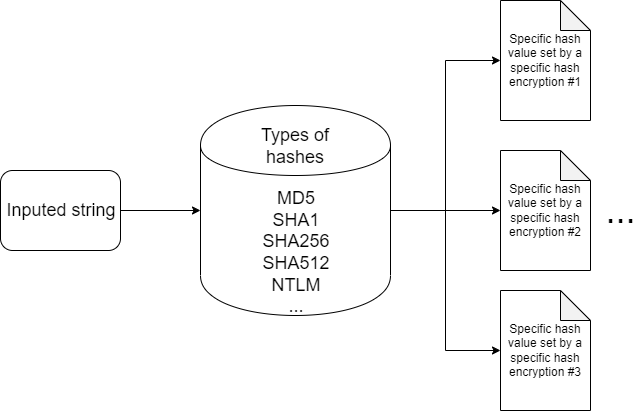
\includegraphics[width=0.9\textwidth]{pngOfDiagrams/hashingExplained.png}
\caption{Hashing mechanism and examples of different hashes}
\end{figure}

The Rabin-Karp method of string matching uses the concept of hashing. The algorithm computes the hash for the selected pattern, then computes the specific hash values for the prefixes of the given text.

In order to calculate the hash value of a substring using prefixes we are going to use the technique of prefix sums. If we have an array of integers that has been constructed using the dynamic programming formula $dp[k] += dp[k - 1]$, for $k=1,\dots,n$, then the sum from an arbitrary index i to an arbitrary index j is equal to $sum(i, j) = dp[j] - dp[i - 1]$. The prefix array is essentially a prefix sum array in this case. Therefore, a hash for a substring that starts at position $i$ and has the length $len = pattern.length()$ is equal to the difference of the prefix of the text that has the length $i + len$ and the prefix that has the length i.   

\begin{figure} [h!]
\centering
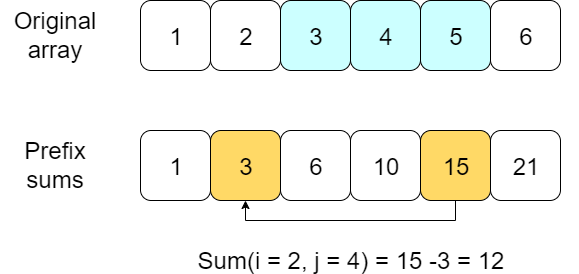
\includegraphics[width=0.68\textwidth]{pngOfDiagrams/prefixSums.png}
\caption{Visualisation of prefix sums}
\end{figure}

A valid implementation of the algorithm that returns an array of the indexes of where the pattern occurs in the given string is: 

\begin{lstlisting}
std::vector<int> rabinKarp(std::string &text, std::string &pattern){
    const int base = 257;
    const long MODULO = 666013;

    // compute the hash value for the pattern

    unsigned long long patternHash = computeValidHash(pattern);

    // compute the hash values for the prefixes of the text
    std::vector<unsigned long long> prefixes(text.length() + 1, 0);
    for(int i = 0; i < text.length(); ++i)
        prefixes[i + 1] = (prefixes[i] + computePosition(text[i]) * precalculatedPowers[i]) % MODULO;

    // find the indexes of the occurences of the pattern in the text

    std::vector<int> result;
    for(int i = 0; i < text.length() - pattern.length() + 1; ++i){
        unsigned long long hashValue = (prefixes[i + pattern.length()] - prefixes[i] + MODULO) % MODULO;
        if(hashValue == patternHash * precalculatedPowers[i] % MODULO)
            result.push_back(i);
    }

    return result;
}
\end{lstlisting}

Note that for the implementation an array of precalculated powers modulo MODULO has been used, in order to reduce the number of calculations needed for computing the correct answer.

Converting strings into integers makes comparing them much easier, comparing their hash values taking O(1) time. Therefore, the time complexity of the Rabin-Karp method is as follows: in order to compute the hash for the pattern the number of calculations required is $O(len(pattern))$, and comparing individual substrings with the hash of the pattern takes $O(len(text))$. Consequently, the overall time complexity of this method takes $O(len(text) + len(pattern))$. 

In order to check the understanding of the technique, consider the following practice problem:

\begin{itemize}
    \item "LPS": Given a string $s$, compute the longest palindromic substring. A string can be defined as a palindrome if it is equal to its reverse.
\end{itemize}

For example, if $s = "dbcba"$, then the longest palindromic substring is $"bcb"$, of length 3. In order to solve this problem, we can use a very clever trick related to string matching. First, the prefix hashes for $s$ will be computed using Rabin-Karp. The second step consists of computing the prefix hashes array for the reverse of $s$ (let's denote it $s'$). Intuitively, when we overlap the strings we can conclude that if the hash for the substring denoted by two arbitrary indices relating to $s$, $i$ and $j$ , is equal to the hash of the substring represented by the indices $i' = len(s) - i - 1$ and $j' = len(s) - j - 1$ in $s'$ (indexing starts at 0), then we found a palindromic substring of length $j - i + 1$.

\begin{figure} [h!]
\centering
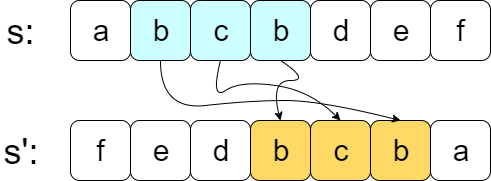
\includegraphics[width=0.68\textwidth]{pngOfDiagrams/reversePrefix.png}
\caption{Correspondence between indices of overlapping strings}
\end{figure}

When constructing the result, we will try to find a possible substring of length equal to the number of characters in the text. If such substring is not found, then the length must be decremented until a valid palindromic substring is found. In the worst case, the longest palindromic substring is equal to just one character from the initial string. This is a first step into reducing the time complexity of this problem from the brute force $O(n^{3})$ to just $O(n^{2})$ by using hash-comparing palindromic search, which can verify a palindrome in $O(1)$. Another spectacular possible ways of solving such problems in $O(n^{2})$ time are using dynamic programming and an 'expand around center' approach, however, achieving a liner time complexity can only be done using Manacher's algorithm, which makes use of the idea of a palindrome occurring in another palindrome. 

\newpage


\subsection{Z-function dynamic search}

\paragraph{}

Z-algorithm belongs to the pattern-matching class of algorithms and concepts and has very special properties. It relies on the technique of dynamic programming and it may be faster in many practical situations that other matching algorithms, such as Rabin-Karp or KMP.

In order to determine the occurrence of of a patter $P$ in a text $T$, a new array of characters will be formed, denoted $S$, $S = P + "*" + T$, where $+$ denotes the concatenation operator of two strings(similarly to strcat() function in C++) and $*$ denotes a character that must not appear in either $P$ or $T$ and has the unique role of separating $P$ from $T$(also called a separator of strings character).

Then a new array $Z$ will be constructed in parallel to $S$, $Z[i]$ denoting maximal length of a sub-sequence that starts at position $i$ in $S$ and it is found at the beginning of $S$. 

\begin{figure} [h!]
\centering
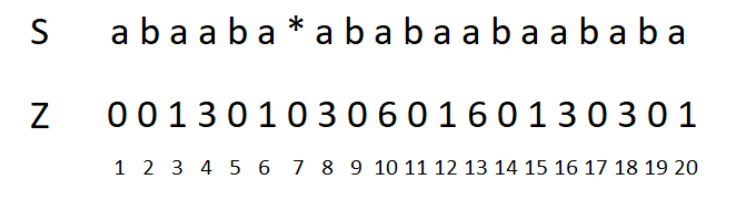
\includegraphics[width=0.8\textwidth]{pngOfDiagrams/zfunction.png}
\caption{Z-function and string concatenation}
\end{figure}

For the sake of simplicity, for this algorithm, indexing starts at 1(the initial position 0 is irrelevant). As a convention, $Z[1] = 0$.

The notion of the Z-box is introduced. The Z-box that starts at position $i$ in the string $S$ is a sub-sequence that start at position $i$ and it is maximal and it is found at the beginning of $S$. Using these notations the problem can be reformulated as the problem of finding all the places $i$ that satisfy the condition: 

$$
Z[i] = len(P) = m
$$

If $i$ is a place for which the condition is fulfilled, then $P$ is found as a sub-sequence in $T$ at position $i - m + 1$. For the considered example, $Z[10] = 6$ and $Z[12] = 6$, which implies that $P$ is found in $T$ at positions 3 and 5.

The main objective is computing the string $Z$ in just one iteration of $S$ from the index 2 to the index $m + n + 1$ in linear time.

In order to achieve a linear time complexity $O(n + m)$, two new variables are introduced:

\begin{itemize}
    \item $R$ - the right boundary (the end) of the Z-box.
    \item $L$ - the left boundary (the beginning) of the same Z-box.
\end{itemize}

Suppose that the values of $Z[1], Z[2], \cdots ,Z[k - 1]$ were determined and that the next term that needs to be computed is $Z[k]$. For this step, some cases need to be considered:

\begin{itemize}
    \item Case 1: $k > R$
\end{itemize}

In this case the value of $Z[k]$ needs to be determined explicitly ("two finger algorithm", two indexes starting at $left = 1$ and $right = k$ and if $S[left] = S[right]$ then left and right are incremented). Computing $Z[k]$ may lead to modifications of $L$ and $R$.

\begin{itemize}
    \item Case 2: $k \leq R$
\end{itemize}

\begin{figure} [h!]
\centering
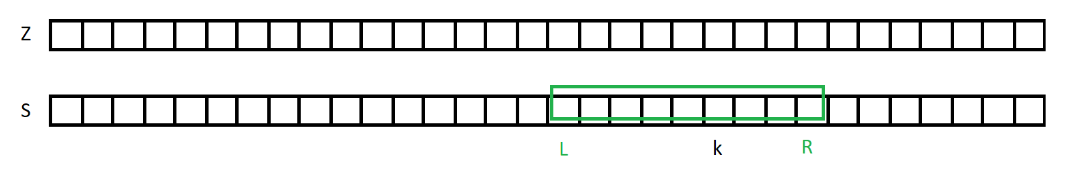
\includegraphics[width=1\textwidth]{pngOfDiagrams/zalgo1.png}
\end{figure}

The portion delimited by $L$ and $R$ is noted with $a$. By definition, $a$ is also found at the start of $S$. The corespondent of $k$ in the beginning section is noted with $k' = k - (L - 1)$.

\begin{figure} [h!]
\centering
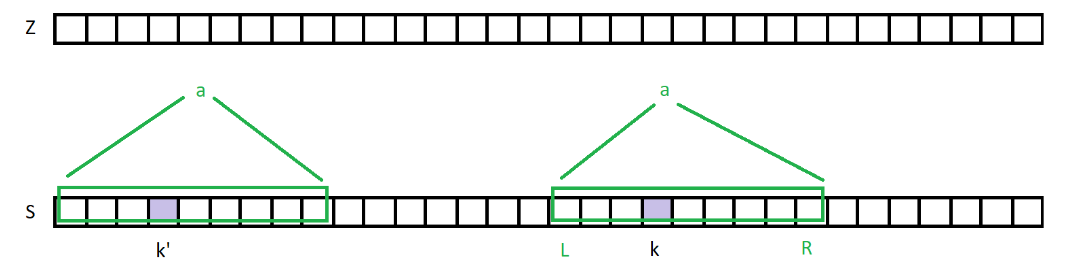
\includegraphics[width=1\textwidth]{pngOfDiagrams/zalgo2.png}
\end{figure}

The region between $k$ and $R$ is noted with $b$ ($k$ and $R$ inclusive).

\begin{figure} [h!]
\centering
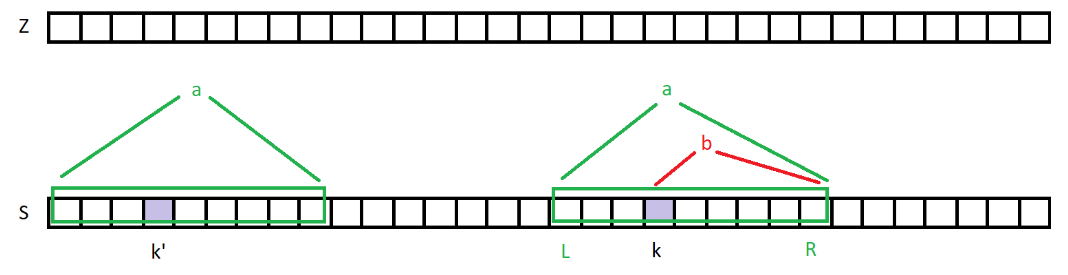
\includegraphics[width=1\textwidth]{pngOfDiagrams/zalgo3.png}
\end{figure}

\newpage

\begin{itemize}
    \item Case 2 a): $Z[k'] < len(b)$
\end{itemize}

In this case $Z[k] = Z[k']$ (immediate determination) since $x \neq y$.

\begin{figure} [h!]
\centering
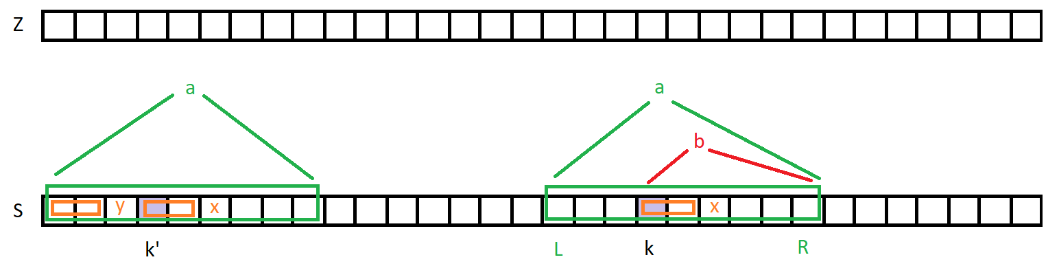
\includegraphics[width=1\textwidth]{pngOfDiagrams/zalgo4.png}
\end{figure}

\begin{itemize}
    \item Case 2 b): $Z[k'] > len(b)$
\end{itemize}

In this case $Z[k] = len(b)$, because $x \neq y$.

\begin{figure} [h!]
\centering
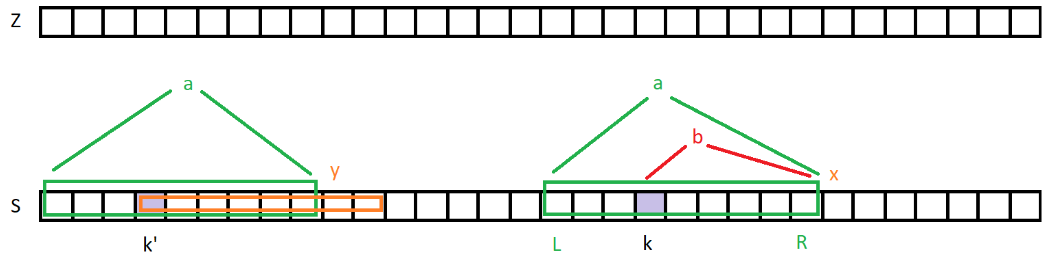
\includegraphics[width=1\textwidth]{pngOfDiagrams/zalgo5.png}
\end{figure}

\begin{itemize}
    \item Case 2 c): $Z[k'] = len(b)$
\end{itemize}

In this case $Z[k]$ is determined using the "two fingers" method. Computing $Z[k]$ may lead to modifications of $L$ and $R$.

As seen, this technique relies on dynamic programming, by computing the next terms (when possible) using past results.

Now for the classical problem implementation:


\begin{itemize}
    \item Given a string, compute its corresponding Z-vector.
\end{itemize}

\begin{lstlisting}
void Z(){
    char S[NMAX];
    int Z[NMAX];
    int n, l, r;
    std::cin >> S + 1;
    n = strlen(S + 1);
    Z[1] = 0;
    l = 0;
    r = 0;
    for (int k = 2; k <= n; k++)
        if (k > r){
            // two fingers
            int left, right;
            left = 0;
            right = k - 1;
            while (S[left + 1] == S[right + 1]){
                ++left;
                ++right;
            }
            Z[k] = left;
            if (left >= 1){
                l = k;
                r = right;
            }
        }
        else{
            int kp;
            kp = k - (l - 1);
            if (Z[kp] < r - (k - 1))
                Z[k] = Z[kp];
            else if (Z[kp] > r - (k - 1))
                Z[k] = r - (k - 1);
            else{
                /// two fingers
                int left, right;
                left = r - (k - 1);
                right = r;
                while (S[left + 1] == S[right + 1]){
                    ++left;
                    ++right;
                }
                if (right > r)
                {
                    l = k;
                    r = right;
                    Z[k] = right - (k - 1);
                }
            }
        }
    for (int i = 1; i <= n; ++i)
        std::cout << Z[i] << ' ';
}
\end{lstlisting}


\newpage

\subsection{Finite automata}

\paragraph{}

A finite automata(or a finite-state machine) is defined as a behavioural model made of a finite number of states, transitions and actions. 
%mathematical model of finite automata

Finite-state machines have many implications, ranging from the basics of artificial intelligence, to theoretical applications in mathematical problems. This chapter will treat finite automata from the perspective of string matching and manipulation and aims to introduce the reader to a concept that is the foundation for string theory. 

A finite automata can be viewed as a quintuple of objects and is defined using the following mathematical model:

\begin{itemize}
    \item $Q = \{ q_0, q_1, \dots , q_n \}$, a finite set of states
    \item $q_0$, $q_0 \in Q$ ,the initial state of the machine
    \item $A, A  \subseteq Q$, the set of acceptation states
    \item $\Sigma$, an alphabet
    \item $\delta : Q \times \Sigma \rightarrow Q$, the transition function of the finite automata
\end{itemize}

Two groups of finite-state machines are defined: acceptors and transducers. Acceptors are the type of finite automata that produce a binary output, answering the simple question: "Is the entry accepted or not by the constructed behavioural machine?". If at the end of processing the input, the machine is in a final (terminal) state, then the input is accepted by the machine, otherwise it is not. Transducers give an output based on the selected input, using actions and are also classified into two categories: the Moore machine and the Mealy machine.

The model of finite automata for string manipulation is classified as an acceptor, since we only need a binary "Yes" or "No" to determine whether the given string is accepted by the machine. A nice idea would be representing the finite automata as a directed graph, the nodes representing the states of the machine and the edges the connection between them. Firstly, we are going to define a simple machine that outputs "Yes" if and only if the given input is the string "hello" in order to demonstrate the main principle.

\begin{figure} [h!]
\centering
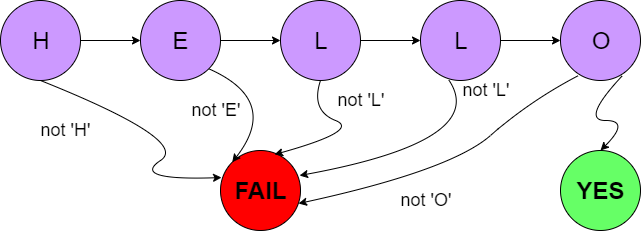
\includegraphics[width=0.87\textwidth]{pngOfDiagrams/finiteautomatasimple.png}
\end{figure}

Now the next logical step would be constructing a finite state machine that would accept multiple strings. The finite state machine can be constructed as a graph where the nodes denote the states and the edges the valid connections between them, where the transition function will be explicitly given.

\begin{figure} [h!]
\centering
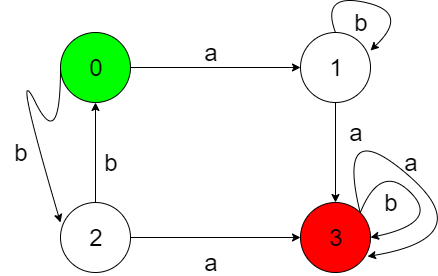
\includegraphics[width=0.73\textwidth]{pngOfDiagrams/finiteautomatacomplex.png}
\end{figure}

% enuntare functie de tranzitie 
% enuntare state de inceput si de final
% enuntare legatura cu KMP ul 
% enuntare logica de functionare
% enuntare diferite stringuri acceptare
% enuntare delta(delta(delta...
% cod pentru utilizare automat finit 
% tranzitie pentru capitolul de kmp

As seen in the example, the beginning state is denoted by the $'0'$ node, and the end-state is denoted by the node $'3'$. Every input that is tested using this automaton and ends in the third state is considered accepted by the constructed machine. The connection between the finite states are defined by the transition function $\delta$:

\begin{itemize}
    \item $\delta (0, a) = 1$
    \item $\delta (0, b) = 2$
    \item $\delta (1, a) = 3$
    \item $\delta (1, b) = 1$
    \item $\delta (2, a) = 3$
    \item $\delta (2, b) = 0$
    \item $\delta (3, a) = 3$
    \item $\delta (3, b) = 3$
\end{itemize}


The transition function translates as such: for a current state(denoted by the first argument of the function), the following character in the string can either switch the current state, or remain on said state. In order to comprehend the concept, consider the following input that is tested against a finite automata described by the mentioned transition function. If the input is $"bbaba"$, then the following behaviour is expected from the automata:

\begin{itemize}
    \item $\delta (0, b) = 2$, from state $'0'$, based on input $'b'$, the current state is now state $'2'$
    \item $\delta (2, b) = 0$, from state $'2'$, based on input $'b'$, the current state is now state $'0'$
    \item $\delta (0, a) = 1$, from state $'0'$, based on input $'a'$, the current state is now state $'1'$
    \item $\delta (1, b) = 1$, from state $'1'$, based on input $'b'$, the current state is now state $'1'$
    \item $\delta (1, a) = 3$, from state $'a'$, based on input $'a'$, the current state is now state $'3'$, the final state.
\end{itemize}

So, for the input $"bbaba"$ that is "fed" to the automata, the final state is state $'3'$, which is also part of the end-states of the machine $A$. That means that the automata accepts this input. By construction, this automata can accept multiple inputs, such as $"aaaaaaa"$ or $"aabababab"$. On the other hand, the input $"bba"$ would not be accepted by the finite-state machine, since the final state after the given input will be state $'1'$ (as seen in the diagram). In general form, if there is a string denoted $t$, $len(t) = p$, then the string is accepted if and only if:

$$
\delta ( \dots \delta ( \delta (0, t[0]), t[1] ) \dots, t[p - 1]) \in A
$$

% cod pentru utilizare automat finit 

As a general template, once the transition function $\delta$ is specifically defined for a task, testing whether a string is accepted by the automaton becomes rather trivial:

\begin{lstlisting}
bool isAcceptedByAutomata(int initialState, std::string text){
    int n = text.length();
    int currentState = initialState;
    for(int i = 0; i < n; ++i){
        currentState = delta(currentState, text[i]);
    }
    return (currentState == acceptanceState);
}
\end{lstlisting}

% tranzitie pentru capitolul de kmp

Now the reader may be pondering the question: why is finite automata important in string matching? At a basic level, a lot of string-matching algorithms are based on constructing a specific automaton, then querying the machine in order to find the appearance of a pattern into a text. In fact, the Knuth-Morris-Pratt (for short, KMP) string-searcher is based on the concept of finite automata, where the $\pi$ table construction is similar to building such machine, but that's a topic for another chapter. 

In order to see a practical application of the finite automata, consider the next problem:

\begin{itemize}
    \item Strange Dialogue: Two friends, $A$ and $B$ are having a conversation of length $m$, defined as a random succession of the next words: out, output, puton, in, input, one. In their dialogue there are no blank spaces. Given an input, determine if the input is a possible dialogue between the two friends.

    As an example, "oneputonininputoutoutput" would be a valid dialogue and "inonputin" would be an invalid input.
\end{itemize}

After careful consideration, we need to determine whether the input is a concatenation of the words above. The problem can be approached by using dynamic programming, by constructing an auxiliary array, $V$, with boolean elements ($0$ or $1$) possible values for $V_i$ ($V_i = 1$ if $ V_{1 \dots i}$ is a valid dialogue, $0$ if not). But there is a more elegant approach based on finite automata.

A great idea would be constructing an acceptor-type finite automata. With its help, the text analysis will be made from $V_{m - 1}$ to $V_0$, constructing by hand the transition function. $0$ serves as the beginning state and also the acceptance state. The finite-state machine can be seen as such:

\begin{figure} [h!]
\centering
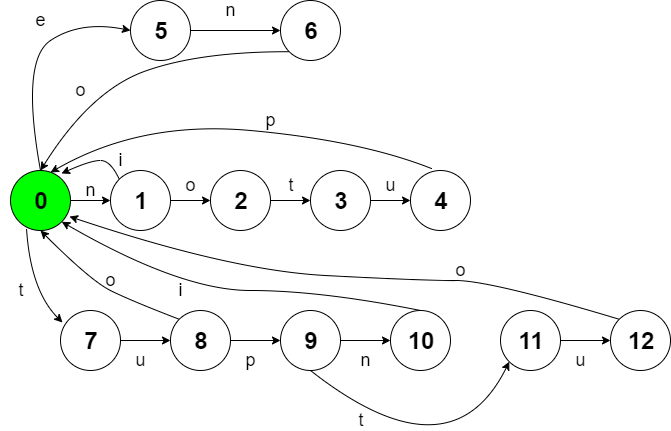
\includegraphics[width=1\textwidth]{pngOfDiagrams/strangedialogue.png}
\end{figure}


Based in this definition, the implementation is rather trivial:

\begin{lstlisting}
int delta(int q, std::string c){ // current state and next character
    switch(q){
        case 0: if(c == "n")
                    return 1;
                if(c == "e")
                    return 5;
                if(c == "t")
                    return 7;
                return -1; // if the conditions aren't met

        case 1: if(c == "i")
                    return 0;
                if(c == "o")
                    return 2;
                return -1;

        case 2: if(c == "t")
                    return 3;
                return -1;

        case 3: if(c == "u")
                    return 4;
                return -1;

        case 4: if(c == "p")
                    return 0;
                return -1;

        case 5: if(c == "n")
                    return 6;
                return -1;

        case 6: if(c == "o")
                    return 0;
                return -1;

        case 7: if(c == "u")
                    return 8;
                return -1;

        case 8: if(c == "o")
                    return 0;
                if(c == "p")
                    return 9;
                return -1;

        case 9: if(c == "n")
                    return 10;
                if(c == "t")
                    return 11;
                return -1;

        case 10: if(c == "i")
                    return 0;
                return -1;

        case 11: if(c == "u")
                    return 12;
                return -1;

        case 12: if(c == "o")
                    return 0;
                return -1;
    }
    return -1;
}

void solve(){
    q = 0; // starting state
    for(int i = m - 1; i >= 0; --i){
        q = delta(q, text[i]);
        if(q == -1)
            break;
    }
    if(q == 0) // it has ended in the acceptance state 
        std::cout << "Valid";
    else 
        std::cout << "Invalid";
}
\end{lstlisting}


We hope that this chapter serves as a brief introduction to the core concepts of string matching that apply to higher-level string manipulation concepts and methods. Note that almost every entity can be seen as a finite automata and can be modelled as a graph, so this chapter also serves as a basic foundation for a concept that can be applied to a vast variety of problems. 

\newpage

\subsection{Word Trie model}

\paragraph{}

A trie is a powerful data structure and a key-concept regarding string searching and manipulation. Outside of the realm of strings, tries have many applications in solving different types of problems.

In order to organically discover the trie, consider the following problem:

\begin{itemize}
    \item Several operations regarding a list of strings are defined.
    \begin{itemize}
        \item $(0, W)$, insert the string $W$ in the list
        \item $(1, W)$, delete an appearance of $W$ from the list
        \item $(2, W)$, print the number of appearances of the word $W$ in the list
        \item $(3,W)$, print the length of the longest common prefix of $W$ with any word from the list.
    \end{itemize}
\end{itemize}

A brute force approach after some analysis of the problem performs to many calculations and is based on simulating the operations according to the definition, by defining a list. Consequently, operations $0$ and $1$ are computed in $O(len(W))$, and operations $2$ and $3$ are computed in $O(n \times len(W))$, since a full iteration of the list is necessary for solving this type of query. This is far from optimal.

The main problem here is with operation number $3$. Suppose operation $3$ din not exist. How can the problem be solved then? The problem is reduced to constructing a red-black tree for the list of the words and then querying it. A red-black tree can be defined as a self-balancing binary tree, where each nodes stores extra data containing its respective color(either red or black). These trees have some important properties that match our operations: every node is either red or black, all NULL nodes are considered black, a red node does not posses a red child and every path from a node to any of its descendant NULL node goes through the same number of black nodes.

\begin{figure} [h!]
\centering
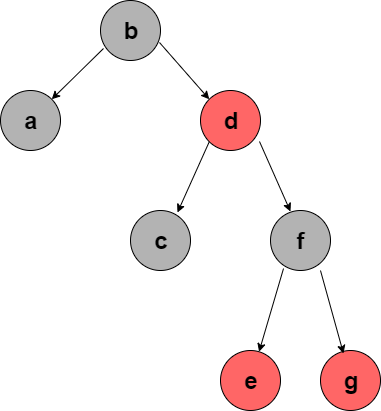
\includegraphics[width=0.45\textwidth]{pngOfDiagrams/redblacktree.png}
\end{figure}

\newpage

The map data structure in C++ is implemented using red-black trees. So, for the first tasks of the problem, the problem becomes trivial by using the map data structure, which has a key (the word itself) and a value(the frequency of the word). This does not solve however the last task.

As an example, consider the following strings: "team", "teach", "tea", "tea", "top", "big" and "bag". What if, when constructing an arborescent data structure, instead of identifying the keys through the information in a single node, we identify the keys through the path from the root of the tree to a specific node?

\begin{figure} [h!]
\centering
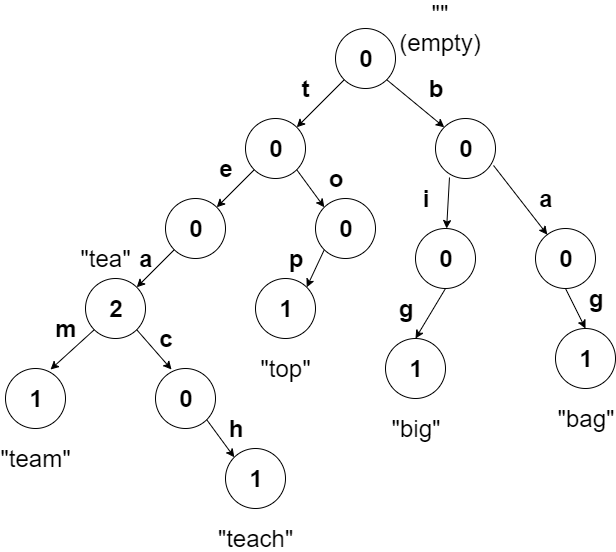
\includegraphics[width=0.82\textwidth]{pngOfDiagrams/trie}
\end{figure}

As seen in the example, the information in the node denotes the number of strings that end in that specific node. For example, the string "tea" is given twice in the input, so the node's associated value is 2. Starting from the root(who is associated to an empty string), every node will store information about the key which is obtained by concatenating all of the edges that lead to it. With this data structure, every operation can be computed in $O(len(word))$, which is excellent. As for the space complexity, the trie will never hold more than $O(totalLength \cdot len(\Sigma))$, where $\Sigma$ is the alphabet(in our case, $len(\Sigma) = 26$).

This concept can very easily be used and adapted for our problem. Now the fourth task becomes trivial: starting from the root, go down until you cannot anymore with the letters of the current word $W$. Consequently, the result would be the number of nodes visited until we can't go down anymore. In order to represent this specific data structure, dynamic memory allocation will be used.

For the implementation, the trie will have a count that stores the number of words that end in the current node and a count for the number of words that have passed through a node without ending in it. In the constructor, those variables are set to 0.

\begin{lstlisting}
const int SIGMA = 'z' - 'a' + 1; // the length of the alphabet

struct trieNode {
    int end_count; // number of words that end in the current node
    int passing_count; // number of words that pass through this node
    
    trieNode *sons[SIGMA];

    trieNode() { //constructor
        end_count = 0;
        passing_count = 0;
        memset(sons, 0, sizeof(sons)); // every son is NULL
    }
};
\end{lstlisting}

After the structure was declared, four operations need to be declared (remove, insert, frequency, longest common prefix), according to the needs of the problem.

\begin{lstlisting}
// from the root we insert string s starting from pos
void insert(trieNode *root,
    const std::string &s, int pos) {
    root -> passingCount += 1;
    if (pos >= (int) s.size()) {
        root -> endCount += 1;
        return;
    }
    int sonIndex = s[pos] - 'a';
    if (root -> sons[sonIndex] == NULL) {
        root -> sons[sonIndex] = new trieNode();
    }
    insert(root -> sons[sonIndex], s, pos + 1);
}

void remove(trieNode *root,
    const std::string &s, int pos) {
    root -> passingCount -= 1;
    if (pos >= (int) s.size()) {
        root -> endCount -= 1;
        return;
    }
    int sonIndex = s[pos] - 'a';
    remove(root -> sons[sonIndex], s, pos + 1);
}

int getFrequency(trieNode *root,
    const std::string & s, int pos) {
    if (pos >= (int) s.size()) {
        return root -> endCount;
    }
    int sonIndex = s[pos] - 'a';
    if (root -> sons[sonIndex] == NULL) {
        return 0;
    }
    return getFrequency(root -> sons[sonIndex], s, pos + 1);
}

int getLCP(trieNode *root,
    const std::string &s, int pos) { /// longest common prefix
    if (pos >= (int) s.size()) {
        return 0;
    }
    int sonIndex = s[pos] - 'a';
    if (root -> sons[sonIndex] == NULL || root -> sons[sonIndex] -> passingCount == 0) {
        return 0;
    }
    return 1 + getLCP(root -> sons[sonIndex], s, pos + 1);
}
\end{lstlisting}

After these operations are constructed, the final step is just calling those functions for the type of operation that we need:

\begin{lstlisting}
void solve(){
    int op;
    std::string s;

    trieNode *root = new trieNode();

    while (std::cin >> op >> s) {
        if (op == 0) {
            insert(root, s, 0);
        } else if (op == 1) {
            remove(root, s, 0);
        } else if (op == 2) {
            std::cin << getFrequency(root, s, 0) << "\n";
        } else {
            std::cin << getLCP(root, s, 0) << "\n";
        }
    }
}
\end{lstlisting}

This is considered the classical application of a trie for a list of words. However, this data structure is very powerful and can be hidden in many problems.

\begin{itemize}
    \item Given an array of integers $a_1, a_2, \dots, a_n$, determine a sub-sequence such that $a_i \oplus a_{i + 1} \oplus \dots \oplus a_j$ has a maximum value, where $\oplus$ denotes the XOR operation.
\end{itemize}

The XOR ("exclusive or") denotes symmetric difference in computer science. This operation also has some special properties that can be deduced after analysing the logic table.

\begin{figure} [h!]
\centering
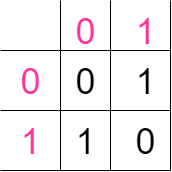
\includegraphics[width=0.3\textwidth]{pngOfDiagrams/xorgate.png}
\caption{XOR logic table}
\end{figure}

\begin{itemize}
    \item $a \oplus 0 = a, \forall a \in {N}$, 0 is the neutral element for XOR.
    \item $a \oplus a = 0, \forall a \in {N}$
\end{itemize}

When analysing this problem, we can recognize a pattern. Suppose that the XOR operation was replaced by addition. Then the problem would be easily solved by using the technique of prefix sums. Then, the result would be of the form $DP_{j} - DP_{i - 1}$, where $DP$ denotes the prefix sum array. By using this thought process, can we translate the idea to work on the operator $\oplus$? Can we model the problem in such a manner that we would have a formula similar to the prefix sums? 

$$
a_{i + 1} \oplus a_{i + 2} \oplus \dots \oplus a_j = DP_j \oplus DP_i
$$

Now the problem translates to finding the best left index $i$ for a fixed end $j$. Looking at the binary representation of $DP_j$, if its most significant bit is $k$, then, if possible, we would choose the first bit of $DP_i$ to be $\neg k$, since $k \oplus \neg k = 1$. This guarantees a larger sum than choosing the current bit to be equal to $k$, since $k \oplus k = 0$. This process continues for every bit of in the binary representation of an integer.

While not evident at first sight, this problem can be implemented using a trie, which will store every binary representation of the numbers inside the $DP$ "prefix xors" array. For example, if $A = [1, 0, 5, 4, 2]$ then $DP = [0, 1, 4, 0, 2]$. The suffix trie associated with the $DP$ array would be:

\newpage

\begin{figure} [h!]
\centering
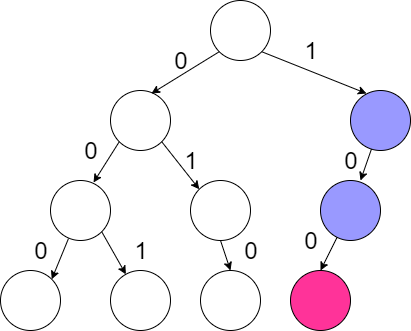
\includegraphics[width=0.54\textwidth]{pngOfDiagrams/xormax (1).png}
\end{figure}

In this particular example, for $DP_{4} = 2$, the purple nodes represent the free choice and the pink node denotes a forced choice. $DP_4 \oplus DP_2$ is the maximum value that can be obtained, in this case $4 \oplus 2 = 6$, and it is obtained for $i = 4 - 1 = 3$ and $j = 4$ in the original array. This problem is a great example of the practical usage of a trie. In the current context, the alphabet $\Sigma$ was seen as only having the binary digits $0$ and $1$ and a trie was constructed using this particular paradigm. The overall time complexity is $O(n \log n)$ ($n$ trie iterations, height of the trie being denoted by the logarithm).

\newpage



\newpage

\subsection{PI tables. Knuth-Morris-Pratt}

\paragraph{}

The task remains the same: given a string of characters (let it be called $s$), find the positions of a given pattern(let it be called $p$) that occurs inside the string $s$.

The Knuth-Morris-Pratt matcher is a method of string searching which revolves around the idea of computing a "$\pi$ table" in order to skip some string matching computations by using previous results. The central idea of computing $\pi$ is looking at all the prefixes of the given pattern that are also suffixes of the same pattern substring. By using this $\pi$ array, the time complexity is reduced to $O(len(s) + len(p))$, so it reaches a linear time complexity. Fundamentally, the $\pi$ table is defined as follows: 

$$
    \pi[i]=max(p[1,\dots \pi[i]] \ is \ suffix \ of \ p[1,\dots i]]) < i
$$

In order to understand the the concept of such tables and try to develop an optimal solution for generating them, consider the following example:

% diagrama de la slideul 11 de pe prezentarea powerpoint

\begin{figure} [h!]
\centering
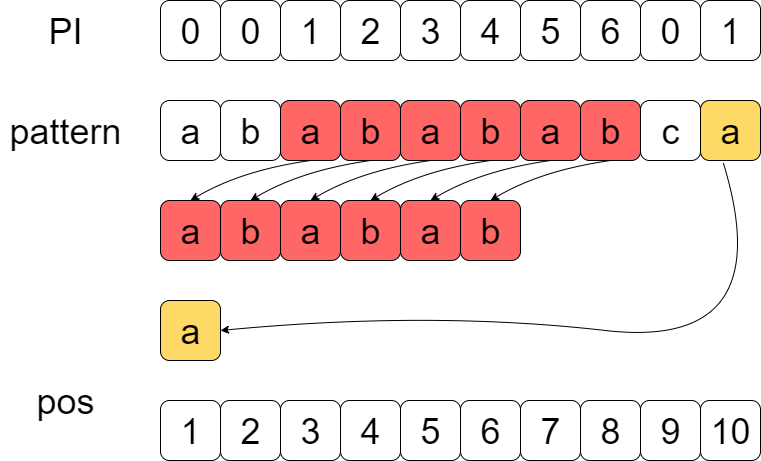
\includegraphics[width=0.8\textwidth]{pngOfDiagrams/KMPPI.png}
\caption{PI table construction logic example}
\end{figure}

In order to understand the concept of $\pi$ tables, we have to understand this construction. For example, $\pi[6] = 4$ because the substring $"abab"$ is a valid suffix for $"ababab"$. On the same logic, the null values in the $\pi$ table are constructed on the logic that there doesn't exist a prefix of length strictly smaller than $i$ that ends with $p[i]$.  

Based on this intuitive example, we can make some useful observations on the respective $\pi$ table. Firstly, we can conclude that if $p[1,\dots \pi[i]]$ is a suffix of $p[1,\dots i]$, then $p[1,\dots \pi[i]] - 1$ is also a suffix of $p[1,\dots i - 1]$. Secondly, as an observation, some fundamental recurrences appear if analyzing the construction of the respective table for the said pattern.


% algoritm trivial pentru construirea tabloului PI

An intuitive trivial construction of a $\pi$ table for a specific pattern won't however achieve the desired time complexity, not without some key observations in order to optimize it. Such basic implementation of this table is as follows: 

\begin{lstlisting}
// returns the substring from pos start to pos fin
std::string substring(std::string &s, int start, int fin){
    std::string result;
    for(int i = start; i < fin; ++i)
        result += s[i];
    return result;
}

// basic implementation for the creation of PI table
std::vector<int> piTable(std::string &text){
    std::vector<int> result(text.length());
    for(int i = 0; i < text.length(); ++i)
        for(int k = 0; k <= i; ++k)
            if(substring(text,0, k) == substring(text, i - k + 1, i + 1))
                result[i] = k;
    return result;
}
\end{lstlisting}

The lazy implementation of the $\pi$ table has a time complexity of $O(n^3)$, which is not optimal at all. This algorithm is built strictly by using the description: for each valid position $i$ in the text, we take another index $k$ that increments up to the said position, and then we compare the resulting substrings, the first substring starting at position 0 and ending at position $k$ and the second one starting at position $i - k + 1$ and ending at position $i + 1$ (note that both substrings have the length equal to $k$). 

After careful thought, the optimal implementation for generating a pi table relies on the key observation that we can make use of the already computed data from the previous steps. Note that by definition, $\pi [0] = -1$, so for ease of use we insert at position 0 in the string a character that for sure cannot appear in the text (also called a separator character). 

\begin{lstlisting}
std::vector<int> piTable(std::string &text){
    // note that text indexing starts at position 0
    std::vector<int> result(text.length() + 1, 0);
    result[0] = -1;
    std::string newText = "*" + text; // inserting a separator
    int k = -1;
    for(int i = 1; i <= newText.length() ; ++i){
        while(k >= 0 && newText[k + 1] != newText[i])
            k = result[k];
        result[i] = ++k;
    }
    return result;
}
\end{lstlisting}

%algoritmul kmp 

Now that we were able to compute the $\pi$ table in linear time, we need to somehow correlate it to string matching. By making use of the the said table we can easily conclude that it is possible to "shift" to the right the pattern with $k - \pi [k]$ positions, as this will save a lot of time, eliminating dumb comparisons. This is a very crucial observation in order to correctly construct the algorithm that returns all start positions for a specific pattern in an inputed string: 

\begin{lstlisting}
std::vector<int> KMP(std::string &s, std::string &p, std::vector<int> &PI){
    std::vector<int> startPositions;
    int k = 0;
    for(int i = 1; i <= s.length(); ++i){
        while(k >= 0 && p[k + 1] != s[i])
            k = PI[k];
        ++k;
        if(k == p.length() - 1){
            startPositions.push_back(i - p.length() + 1);
            k = PI[k];
        }
    }
    return startPositions;
}
\end{lstlisting}

% problema semnificativa cu KMP

The KMP is a strong algorithm for pattern matching and it is very versatile. In order to practice the ideas behind it, consider the following problem:

\begin{itemize}
    \item Central European Olympiad in Informatics 2011, Day 1, Gdynia, "Matching".
    As a part of a new advertising campaign, a big company in Gdynia wants to
put its logo somewhere in the city. The company is going to spend the whole
advertising budget for this year on the logo, so it has to be really huge. One
of the managers decided to use whole buildings as parts of the logo.

The logo consists of n vertical stripes of different heights. The stripes are
numbered from 1 to n from left to right. The logo is described by a permutation $(s_{1},s_{2},\dots,s_{n})$ of numbers $1,2,\dots,n$. The stripe number $s_{1}$ is the shortest one, the stripe number $s_{2}$ is the second shortest etc., finally the stripe $s_{n}$ is the tallest one. The actual heights of the stripes do not really matter.

There are $m$ buildings along the main street in Gdynia. To your surprise,
the heights of the buildings are distinct. The problem is to find all positions
where the logo matches the buildings.
Help the company and find all contiguous parts of the sequence of buildings
which match the logo. A contiguous sequence of buildings matches the logo if
the building number $s_{1}$ within this sequence is the shortest one, the building
number $s_{2}$ is the second shortest, etc. For example a sequence of buildings of
heights 5 , 10 , 4 matches a logo described by a permutation ( 3 , 1 , 2), since the
building number 3 (of height 4 ) is the shortest one, the building number 1 is
the second shortest and the building number 2 is the tallest.

The input consists of two integers $n$ and $m$, followed by $n$ integers forming a permutation of the numbers $1,2,\dots,n$. The third line contains $m$ integers $h_{i}$ representing distinct heights of buildings. You should output $k$ integers - 1-based indices of buildings which correspond to the stripe number 1 from the logo in a proper match. The numbers should be listed in an increasing order and separated by single spaces.
\end{itemize}


\begin{figure} [h!]
\centering
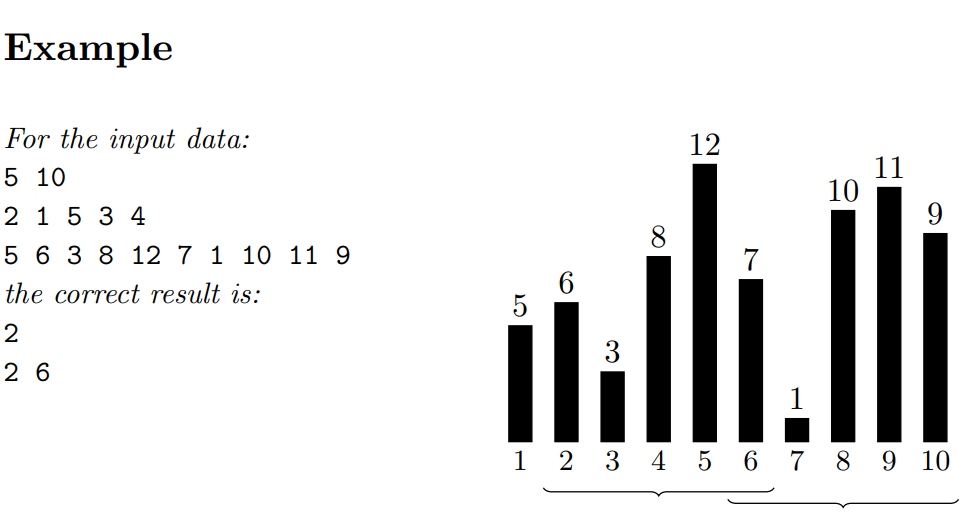
\includegraphics[width=0.87\textwidth]{Problems/GdyiniaMatchingExampleInputOutput.png}
\end{figure}

As seen, both sequences 6,3,8,12,7 and 7,1,10,11,9 match the logo described by the permutation (2,1,5,3,4). In particular, in the first sequence the building number 2(of height 3) is the shortest one, the building number 1 is the second shortest and so on.

At first glance, a solver might not find the relation between this problem and string matching, but after careful consideration, we can make some very useful observations. Firstly, we can view the problem in the context of the theory that was presented and easily correlate both terms: given a text and a pattern, find the occurrence of the pattern in the given string of text. However, the catch in this problem is that both the pattern and the text are represented as numbers, not as a traditional string of characters. At this point, a pertinent question would be where do we see the pattern. 

The trick in this problem is that the pattern is not given, but rather described by the given permutation. So this problem implies a very interesting concept: the existence of multiple patterns that have the same meaning in the current context. Now that we have shaped and driven the thought process, let's expand it further by asking the question: how do we tell if two patterns are equivalent? Intuitively we can define two patterns as being equivalent if for any two positions in the first the values have the same relation $(<, \leq, >, \geq )$ as the values from the same positions in the second pattern. 

As in the preliminary phase of the Knuth-Morris-Pratt, the calculation of the $\pi$ table is mandatory, with the distinction that instead of the strict equality that we had in the original implementation, now we have equivalence. For two substrings, we have equivalence if $text1[i]$ $\omega$ $text1[j]$ if and only if $text2[i]$ $\omega$ $text2[j]$ , $\omega \in \{ <, \leq, >, \geq  \}$. Following the definition of equivalence and the definition of the general construction of the $\pi$ table, the calculation of it becomes trivial and follows the very similar rule:


$$
    \pi[i]=max(equivalence(p[1,\dots \pi[i]],p[1,\dots i]])) < i
$$

After computing the modified $\pi$ table, we have access to the information that we need: for each index how many characters can we extend the general search in order to improve the overall time complexity to the linear $O(n + m)$.

\newpage

\subsection{Suffix Arrays}

\paragraph{}

While the concept may seem abstract at first, suffix arrays play an important role in string manipulation and may lead to further optimisations when working with big data sets.

The suffix array of a given string is defined as an array that contains the indexes of the lexicographically ordered suffixes related to the string. Consider the following construction of a suffix array for the string $"hello"$:


\begin{figure} [h!]
\centering
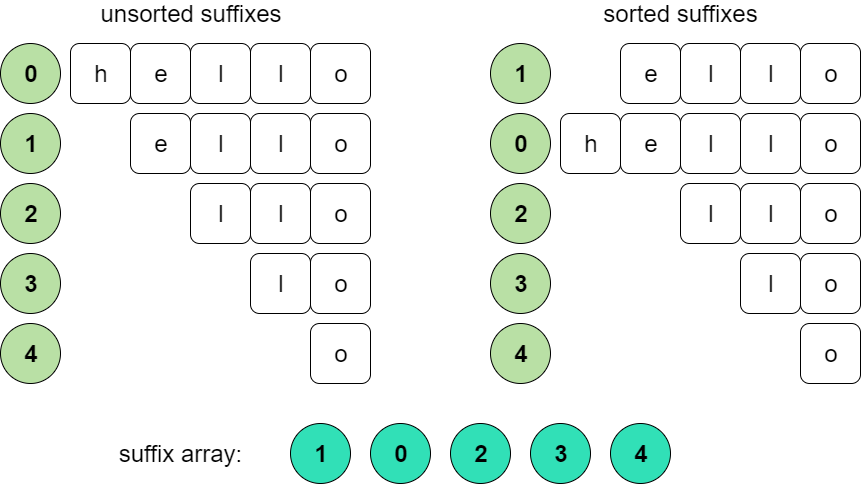
\includegraphics[width=1\textwidth]{pngOfDiagrams/suffixarray1.png}
\end{figure}

The naive approach to the problem is implementing the mechanism without any additional optimisations. The suffixes will be stored and then sorted using an advanced sorting method that takes $O(n \log n)$ time. Since two strings are compared in $O(n)$ time, the overall time complexity will be $O(n^2 \log n)$, which is not optimal. The following implementation makes use of a "different criteria comparison function" that is fed to the standard sort function. In order to store the positions of the suffixes, a structure will be declared.

\begin{lstlisting}
struct suffix{
    std::string info; 
    int pos;
};

bool cmp(suffix &a, suffix &b){ // sorts the std::vector after this specific criteria (lexicographically)
    if(a.info.length() > b.info.length())
        swap(a.info, b.info);
    for(int i = 0; i < a.info.length(); ++i){
        if(a.info[i] < b.info[i])
            return true;
        if(a.info[i] > b.info[i])
            return false;
    }
    return true;
}

std::vector<suffix> suffixArray(std::string text){
    std::vector<suffix> ans;
    // generate all of the suffixes of the given string
    for(int i = 0; i < text.length(); ++i){
        suffix current;
        current.info = "";
        current.pos = i;
        for(int j = i; j < text.length(); ++j)
            current.info += text[j];
        ans.push_back(current);
    }
    sort(ans.begin(), ans.end(), cmp); // sorting using the "cmp" function. sort() accepts a third parameter, which we modified.
    return ans;
}
\end{lstlisting}

This is the naive but convenient approach of computing the suffix array for a given string. The time complexity can be reduced even further. 

A better algorithm consists of keeping track of the lexicographic order of the suffixes of a length that is of the form $2^k$, at every step of $k$. By doing this method, it is clear that the number of steps would be $k = \log n$, where $n$ denotes the length of the given string. Currently, this approach does not lead to a better time complexity. We will worry about that later. In order to understand the optimal approach, it is essential to understand the basic mechanism of sorting the suffixes according to their prefixes of length $2^k$. As an example, consider the string "BOBOGAN". Consider all of the suffixes of the given string. If $2^k$ exceeds the length of the string, we can artificially add a symbol that is the smallest lexicographically and it is not found in the alphabet. This will not impact the result. The standard notation for this symbol is $\$$.

\begin{figure} [h!]
\centering
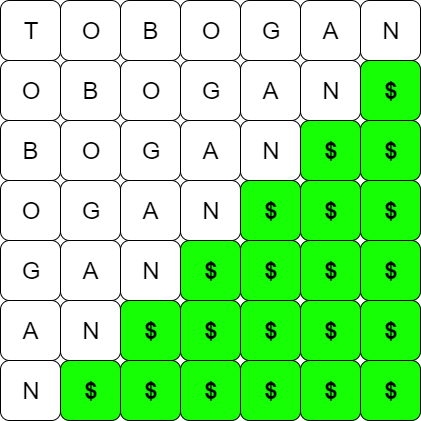
\includegraphics[width=0.40\textwidth]{pngOfDiagrams/suffixarrayex1.png}
\end{figure}

\newpage

As discussed, the first step is sorting in a lexicographical manner the prefixes that have the length $2^0$ (for the first step, $k = 0$) of the suffixes enumerated above. On the right column the lexicographic order at a step $k$ will be stored for every suffix.

\begin{figure} [h!]
\centering
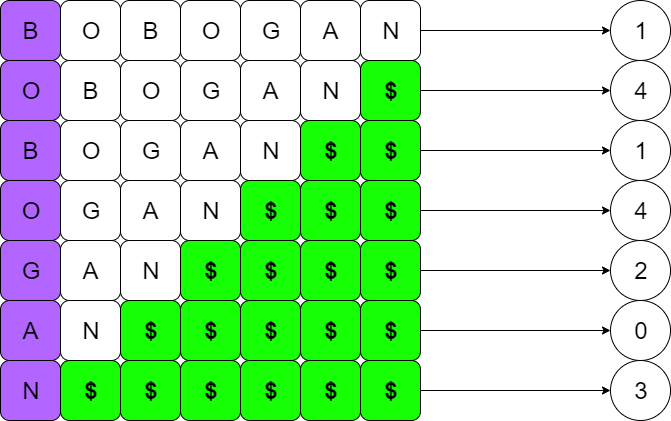
\includegraphics[width=0.7\textwidth]{pngOfDiagrams/suffixarrayex2.png}
\end{figure}

For the first step, for the sorting process, we considered only the first letter of every suffix. The array $[1,4,1,4,2,0,3]$ has been created. Note that at this step, we cannot make a clear lexicographical distinction between the suffixes that start with the same characters, therefore assigning them the same index for now. The next step is $k = 1$, so we need to look at the first $2^1$ characters.

\begin{figure} [h!]
\centering
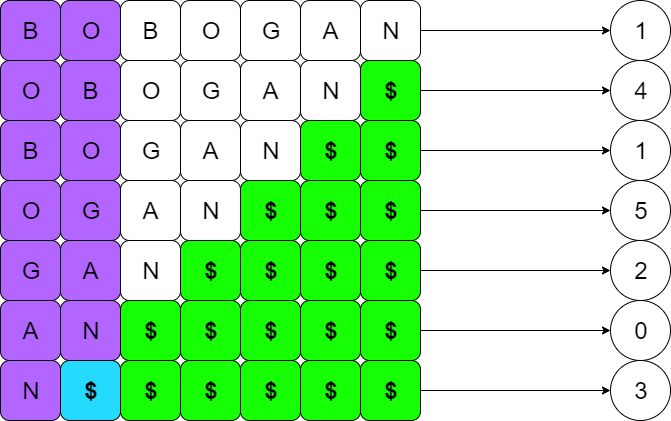
\includegraphics[width=0.7\textwidth]{pngOfDiagrams/suffixarrayex3.png}
\end{figure}

At step $k = 1$ we were able to make a distinction between "OB" and "OG". The process continues for $k = 2$. We need to look at the first $2^2$ characters.

\newpage

\begin{figure} [h!]
\centering
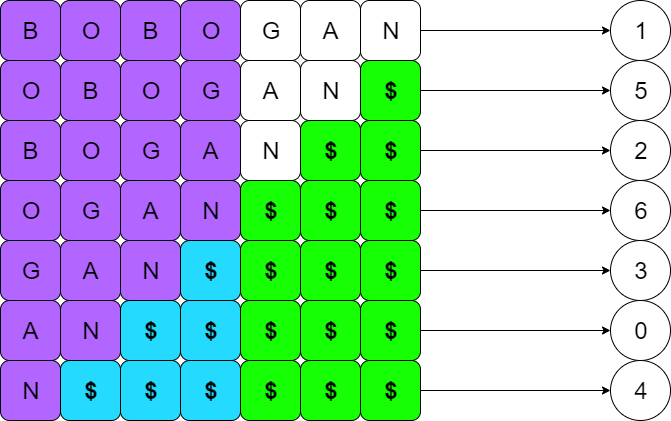
\includegraphics[width=0.7\textwidth]{pngOfDiagrams/suffixarrayex4.png}
\end{figure}

The suffix array has been modified again. The last step is to look at all of the characters of the suffixes.

\begin{figure} [h!]
\centering
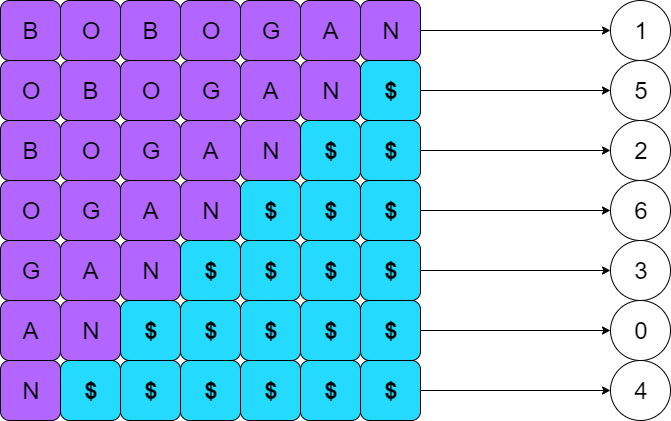
\includegraphics[width=0.7\textwidth]{pngOfDiagrams/suffixarrayex5.png}
\end{figure}

Consequently, the suffix array $[5, 0, 2, 4, 6, 1, 3]$ was built, if we replace the order with their original indexes.

\begin{figure} [h!]
\centering
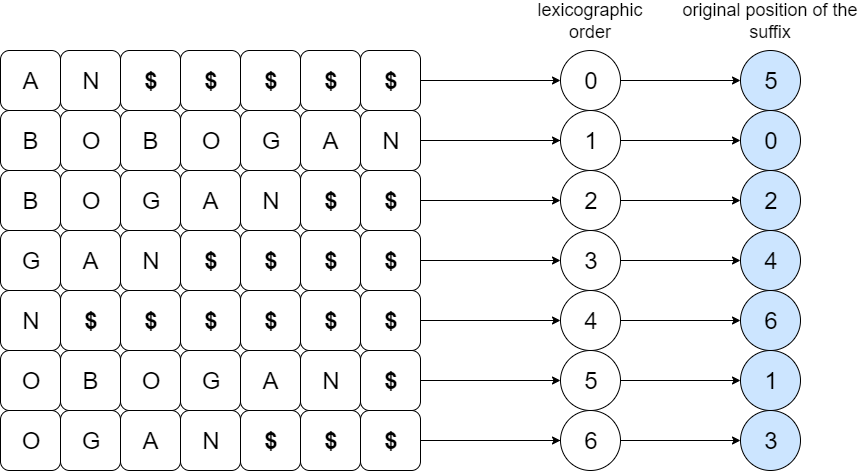
\includegraphics[width=0.8\textwidth]{pngOfDiagrams/suffixarrayex6.png}
\end{figure}

\newpage

By using this thought process, the time complexity can be reduced. A matrix $M$ with $\log n$ lines and $n$ columns will be declared. Denote the input string $T$. $T_{i}^k$ denotes the sub-string of length $2^k$ that starts at index $i$. The position of $T_{i}^{k}$ in the sorted array of the sub-strings $T_{j}^{k}, j = 0, \dots, n - 1$ is kept in the matrix at the position $M_{k,i}$.

In order to optimise this approach, we need to find an efficient way of passing from step $k$ to the step $k + 1$. In order to achieve this, all of the sub-strings $T_{i}^{k}$ are concatenated with $T_{i + 2 ^k}^k$, obtaining the sub-strings of length $2^{k + 1}$. The suffix array will be found on the last line of the matrix $M$.

The overall time complexity of this algorithm would be $O(n \log ^2 n)$, since the sorting process takes $O(n \log n)$ time and the other process is proportional to $O(\log n)$.

\begin{lstlisting}
const int NMAX = (1 << 16); // 2 ^ 16
const int LOGMAX = 20;

struct pairs{ // for every index i a pair of the form P_{k,i} and P_{k, i + 2 ^k} is stored
    int nr[2], p;
} L[NMAX];


char T[NMAX]; // the initial text
int M[LOGMAX][NMAX]; // the matrix. as an observation, only the last two lines can be stored, but then the operation of computing the longest common prefix is not possible

bool cmp(pairs &a, pairs &b){ // compares the pairs after the criteria
    if(a.nr[0] == b.nr[0])
        return a.nr[1] < b.nr[1];
    return a.nr[0] < b.nr[0];
}

void suffixArray(){
    std::cin >> T;
    int N = strlen(T);
    for (int i = 0; i < N; ++i)
        M[0][i] = T[i] - 'a'; // the position of T_i in the sorted array of the characters of T

    for (int k = 1,power = 1; (power >> 1) < N; ++k, power <<= 1) { // upper bound of log_2 n
        for (int i = 0; i < N; ++i) {
            L[i].nr[0] = M[k - 1][i];
            if(i + power < N)
                L[i].nr[1] = M[k - 1][i + power];
            else
                L[i].nr[1] = -1;
            L[i].p = i;
        }
        std::sort(L, L + N, cmp); // the array is sorted in O(n log n)
        // the matrix M(k,i) is built for i = 0, ... n - 1
        for (int i = 0; i < N; ++i)
            if(i > 0 && L[i].nr[0] == L[i - 1].nr[0] && L[i].nr[1] == L[i - 1].nr[1])
                M[k][L[i].p] = M[k][L[i - 1].p];
            else
                M[k][L[i].p] = i;
    }
}
\end{lstlisting}

This method of computing the suffix arrays of a given string stores the matrix, so further applications like computing the longest common prefix of two given sub-strings of another string is possible. If this operation is not required, then instead of the matrix arrays can be used to save up memory.

Note that this implementation can be improved even further, by using a sorting method that takes $O(n)$ time, like radix-sort, which splits the input into "buckets". Radix-sort is supported by this implementation and will reduce the overall time complexity of this algorithm to $O(n \log n)$. We leave this as an appropriate exercise for the reader.

\newpage

\subsection{Aho–Corasick dictionary matching}

\paragraph{}

The previous implementations of string matching algorithms answered the problem of finding a single pattern in a text given text. This was possible in $O(n + m)$ time, where $n$ denotes the length of the text and $m$ denotes the length of the pattern. Now we have the same problem, but instead of matching one singular pattern to a text, we have to find the occurrences of multiple patterns in a text. By matching each individual pattern to the text using any of the described methods(hashing, z-box or KMP), the time complexity will be $O(kn + m)$, where $k$ denotes the number of words in the dictionary, since we have to apply an $O(n + m)$ algorithm a number of $k$ times, for each word in the list.

A better implementation is possible in $O(n + m + o)$, where $o$ denotes all the pattern occurrences from the dictionary in the target text. As a parallel from the classic string searching algorithms, Aho-Corasick can be seen using the black-box principle.

\begin{figure} [h!]
\centering
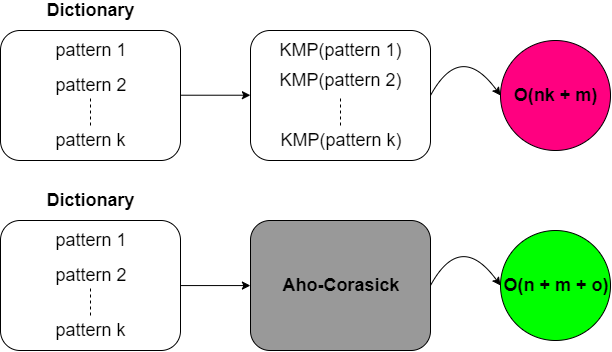
\includegraphics[width=0.95\textwidth]{pngOfDiagrams/aho1.png}
\end{figure}

Now a question rises: how can we reduce the number of computations? Does the dictionary entries have some common characters at certain positions? Is there an efficient way to store the relation between the entries in the dictionary using an appropriate data structure?

At its core, Aho-Corasick constructs a special finite automata, extending the principle of a trie data structure. As a reminder, a trie can efficiently store multiple words from a dictionary. Therefore, Aho-Corasick can be modelled as an finite automata that has the foundation a trie that is constructed using the words in the dictionary. This is a powerful concept, since words in the dictionary can hold many similarities between them, reducing the overall time complexity.

The first step in building an Aho-Corasick finite automata is building a trie with the words in the dictionary. As an example, consider the following dictionary containing $k = 7$ words: "friend", "fraud", "rap", "race", "acid", "circus" and "cider". Therefore, the associated word trie:

\begin{figure} [h!]
\centering
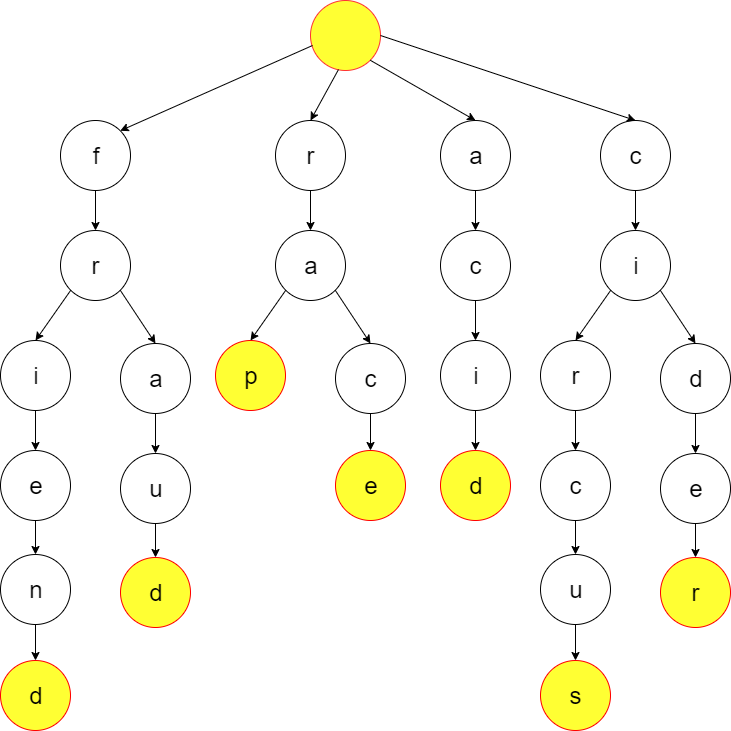
\includegraphics[width=0.90\textwidth]{pngOfDiagrams/aho2.png}
\end{figure}

Now the trie needs to be expanded into a special finite automata according to the theory.

\begin{itemize}
    \item The states $Q$ are represented by the nodes of the trie.
    \item Initial state of the machine is the empty node (the root of the trie).
    \item We can differentiate between three functions that define the Aho-Corasick automata:
    \begin{itemize}
        \item the classic transition function $\delta (q, a)$ that translates the position from the current state to another state by matching target character $a$. If the edge $(q, p)$ has the value $a$, then a correct statement would be $delta(q, a) = p$. Note that the automaton remains at the initial state while scanning non-matching characters ($\delta(0,a) = 0$ if $a$ is not the value of an edge that exits from the root node).

        \item a failure function can be defined. The failure function $f(q)$ for $q \neq 0$ gives the node(state) entered at a mismatch of characters. $f(q)$ is the node that corresponds to the longest proper suffix that is also a prefix of some pattern. This ensures that the automata does not miss any potential occurrences. In the diagram, the failure edges will be represented by the colored lines.

        \item the output function $\Omega(q)$ returns the set of patterns recognised when entering a state $q$.
    \end{itemize}
\end{itemize}

Using this process of thought, an Aho-Corasick automata can be constructed from the previous word trie, where black edges denote the standard $\delta(q,a)$ function and the colored edges belong to the failure function. Edges(non-black) are colored different for a better visualisation, they represent the failure function.

\begin{figure} [h!]
\centering
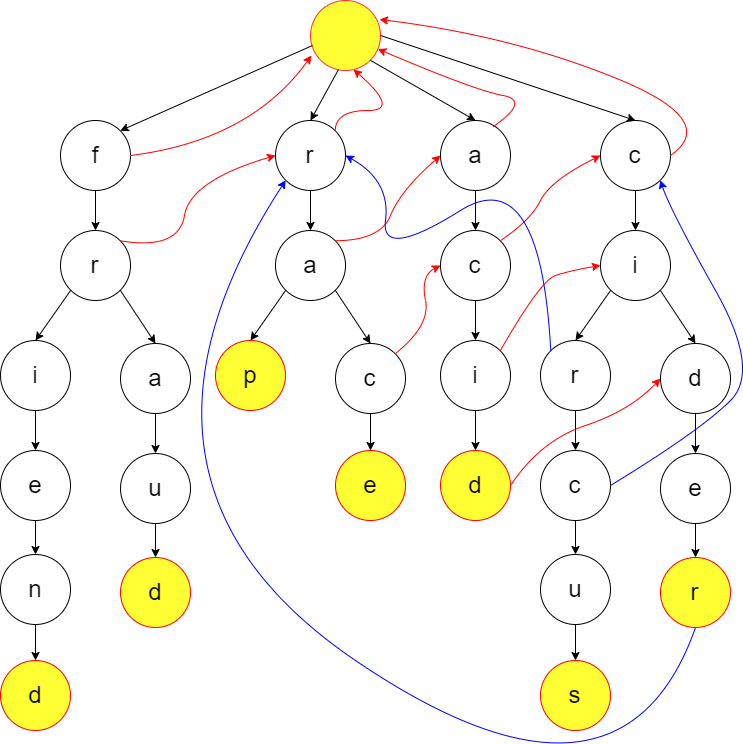
\includegraphics[width=0.90\textwidth]{pngOfDiagrams/aho3.png}
\end{figure}

The automata will spit out how many times a pattern from a dictionary occurs in the target text. For the time complexity, searching the target text using the Aho-Corasick finite automata requires $O(n + o)$, where $o$ denotes the number of pattern occurrences. For each character in the text, the automata performs $0$ or more fail transitions, always followed by a delta transition. Each transition function either moves the depth by 1 or remains at the root node. Fail arrows moves to a closer state to the root node. The $o$ identifier is done in $o \cdot O(1) = O(o)$ time complexity, hence the overall $O(n + m + o)$. For the implementation, consider the following classic implementation problem for the Aho-Corasick automata:

\begin{itemize}
    \item "Dictionary search": Given a string $A$ and an $n$ word dictionary of strings, output for each word in the dictionary the number of occurrences in A.
\end{itemize}

For the actual implementation of the algorithm, the transition function $\delta$ will be built alongside an initialisation of the failure function $f$ and the out $\Omega$ function. The usage of dynamic memory allocation STL containers will be used to represent the transition functions. In the first step the trie will be build alongside the initialisations for the fail and out functions.

\begin{lstlisting}
using namespace std;
const int SIGMA = 'z' - 'a' + 1;

void buildTransition(vector<vector<int>*> &DELTA, vector<int> &FAIL, vector<vector<int>*> &OMEGA, int &no_states, int n) {
    int q;
    string pattern;

    for (int i = 0; i < n; i++) {
        q = 0;
        cin >> pattern;
        for (char c: pattern) {
            int a = c - 'a'; // pos of the character in the alphabet
            if (( *DELTA[q])[a] <= 0) {
                // adding a new state in the finite automata
                DELTA.emplace_back(new vector < int > (SIGMA, -1));
                FAIL.emplace_back(0);
                OMEGA.push_back(nullptr);

                // adding the edge to a new state
                (*DELTA[q])[a] = no_states;
                q = no_states;

                no_states++;
            } else {
                q = (*DELTA[q])[a];
            }
        }
        // initialising the omega out function
        if (OMEGA[q] == nullptr)
            OMEGA[q] = new vector < int > ();
        OMEGA[q] -> push_back(i);
    }
}
\end{lstlisting}

The next step is building the failure function $f$ and the out function $\Omega$. They are computed in a breadth-first (BFS) order, using a queue. Firstly, the queue is empty. For every character $a \in \Sigma$, if $\delta(0, a)$ is equal to $q \neq 0$ then $f(q) = 0$ and $q$ is en-queued. While the queue is not empty, the failure and output functions are built accordingly. $\Omega$ will be built as a reunion of with itself having the argument a fail function.

The nodes closer to the root have already been processed. For a node $u$, $f(u)$ should be the deepest node labeled by a proper suffix of the label of $u$.

\begin{lstlisting}
void buildFailure(vector<vector<int>*> &DELTA, vector<int> &FAIL, list <int> &reverse) {
    list <int> queue;
    for (char c = 'a'; c <= 'z'; c++) {
        int a = c - 'a';
        int next = (*DELTA[0])[a];
        if (next > 0) {
            queue.emplace_back(next);
            reverse.push_front(next);
        }
    }

    while (!queue.empty()) {
        int r = queue.front();
        queue.pop_front();
        for (char c = 'a'; c <= 'z'; c++) {
            int a = c - 'a';
            int u = ( * DELTA[r])[a];
            if (u > 0) {
                queue.emplace_back(u);
                reverse.push_front(u);
                int v = FAIL[r];
                while ((*DELTA[v])[a] == -1)
                    v = FAIL[v];
                FAIL[u] = (*DELTA[v])[a];
                // reunion is based on the FAIL link
            }
        }
    }
}

vector <int> *search(string &text, vector <vector<int>*> &DELTA, vector<int> &FAIL,vector<vector<int>*> &OMEGA){
    int q = 0;
    vector <int> *states_count = new vector <int>(OMEGA.size(), 0);
    vector <int> &count = *states_count;
    count[q] = 1;
    for (char c: text) {
        int a = c - 'a';
        while ((*DELTA[q])[a] == -1)
            q = FAIL[q];
        q = (*DELTA[q])[a];
        count[q]++;
    }
    return states_count;
}

void writeAppearances(vector<vector<int>*> &DELTA, vector <int> &FAIL, vector<vector<int>*> &OMEGA, list <int> &reverse, vector <int> &states_count,int n) {
    vector < int > words_count(n, 0);
    // the reason that nodes are iterated in reverse is to see first when longer words appear(or the words that correspong to a state of a higher depth),which can eventually contain suffixes that correspond to other nodes.
    while (!reverse.empty()) {
        int q = reverse.front();
        reverse.pop_front();

        if (OMEGA[q])
            for (int w: * OMEGA[q])
                words_count[w] += states_count[q];
        // for the state that is a suffix for the string of the state q, for example FAIL[q], we add up how many times it passes through q
        // bottom up
        states_count[FAIL[q]] += states_count[q];
    }
    for (int i = 0; i < n; i++)
        cout << words_count[i] << '\n';
}
\end{lstlisting}

Now that all of the functions are defined, all that remains are some careful initialisations for the dynamically allocated data structures.

\begin{lstlisting}
void solve(){
    string text;
    int n;
    cin >> text >> n;
    // initialise the finite automata with root, example: DELTA[0][_] = 0, FAIL[0] = 0, OMEGA[0] = null
    vector <vector<int>*> DELTA = {
        new vector < int > (26, 0)
    };
    vector <int> FAIL(1, 0);
    vector <vector<int>*> OMEGA = {
        nullptr
    };
    int no_states = 1;
    list<int> reverse;

    buildTransition(DELTA, FAIL, OMEGA, no_states, n);
    buildFailure(DELTA, FAIL, reverse);
    vector <int> *states_count = search(text, DELTA, FAIL, OMEGA);
    writeAppearances(DELTA, FAIL, OMEGA, reverse, * states_count,n);
}
\end{lstlisting}

Aho-Corasick can be a very powerful tool and has many practical applications in the field of string manipulation optimisations and in many fields that require big data comparison(such as the field of genetics, chemistry, etc.). Being modelled after the concept of finite automata, it is very versatile and can be expanded according to different needs.

\newpage

\subsection{Data compression. Burrows-Wheeler transform}

\paragraph{}

In easy terms, data compression is defined as the technique of shortening a string of characters in order to reduce the memory used to store that particular information. In data compression, the information is encoded into a different format from original one using a variety of methods. In order to access the data back at a later time, the process of decoding is used, which translates from the encoded piece of information back to the original information. 

Data compression can be sectioned in two distinct categories: lossless compression and lossy compression. Both types of compression are used in practice and have different applications.
Lossless compression eliminates redundancy in the information that is given. By applying this method of compression, information is not lost during the process of encoding-decoding. This is great for sensitive information where every detail counts. Imagine a database of password hashes that is compressed: every bit of information is important (if only one character is changed then the authentication process won't work). Another great example for lossless data compression would be compressing long strings of DNA in the field of biology. Lossy data compression is generally used when a lossless compression is not possible or when information details are not relevant.

\begin{figure} [h!]
\centering
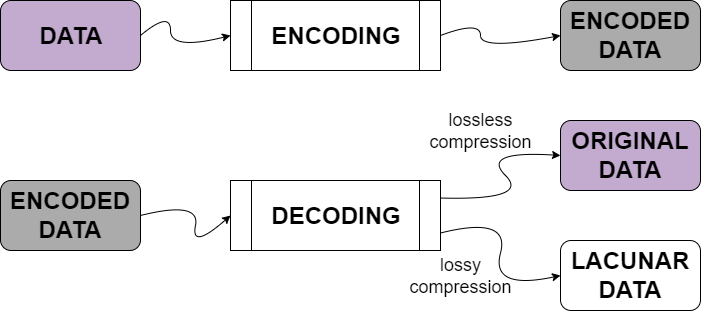
\includegraphics[width=0.85\textwidth]{pngOfDiagrams/compression1.png}
\end{figure}

Data compression requires extra computing time, but it also has a lot of benefits. Other than reducing the memory used, by compressing the data, the time complexity for manipulating and iterating through it is also reduced. This is rather natural, since the amount of data that needs to be iterated through is reduced significantly. For the initial computing power and time of compressing the data, this is a beneficial trade-off in optimising a complex system.

In order to visualise a type of compression, consider the following method of compressing data: when multiple characters of the same kind are stored one next to another, store in the compressed string just a single data value and count. For each sub-string of the same characters of length $k$, store in the encoded text only the length $k$ and the representative character for each bucket.

\newpage

\begin{figure} [h!]
\centering
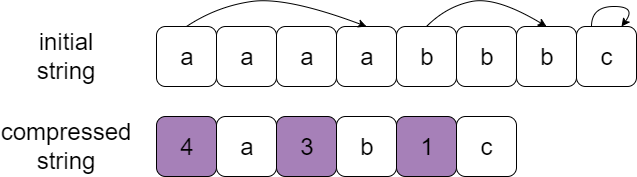
\includegraphics[width=0.85\textwidth]{pngOfDiagrams/compression2.png}
\end{figure}

This form of lossless data compression is called "run-length encoding" (or RLE for short). The main concept of RLE is storing  buckets (or sub-strings) in which the same data value occurs in many consecutive data elements as a single character with its corresponding count. This is one of the most elementary forms of compression and it is still used in image compression. Note that RLE can make the storing space larger if there aren't many sub-strings that contain the same character in consecutive positions, so this compression needs to be used only when the situation is appropriate.

\begin{figure} [h!]
\centering
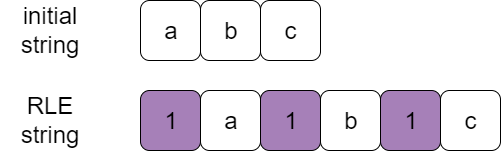
\includegraphics[width=0.65\textwidth]{pngOfDiagrams/compression3.png}
\end{figure}

Many types of compression rely on the fact that the initial string of characters contains sub-strings that only have one unique character. In order to optimise the compression, is there a way to rearrange the initial string in such manner that it benefits greatly from such type of compression method?

In order for the compression to be as effective as possible, the data needs to be pre-processed and transformed in such a manner that it would benefit from traditional compression systems. The Burrows-Wheeler pre-processing transform (BWT for short) aims to rearrange the data into buckets (or runs) of similar characters. BWT is classified as a reversible transformation, the only thing that needs to be stored is only the first original character. This is rather important since after decompression, we want to apply the inverse process of BWT in order to access the original information.

\newpage

\begin{figure} [h!]
\centering
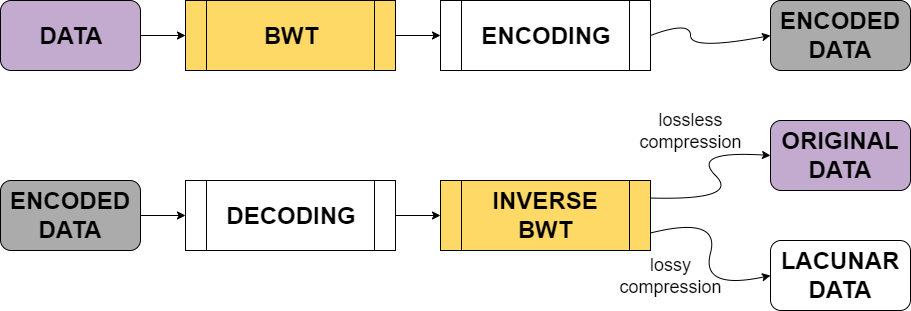
\includegraphics[width=1\textwidth]{pngOfDiagrams/compression4.png}
\end{figure}

The central idea of the BTW is permuting the order of the characters such that identical characters are placed one after another. The transformation consists of sorting the circular shifts of a text in a lexicographic order. After this operation is done, the transformed text is represented by the last column of the matrix read from top to bottom. Consider the following example for the input string "BOBOGAN", where "EOF" denotes the term "end of file".

\begin{figure} [h!]
\centering
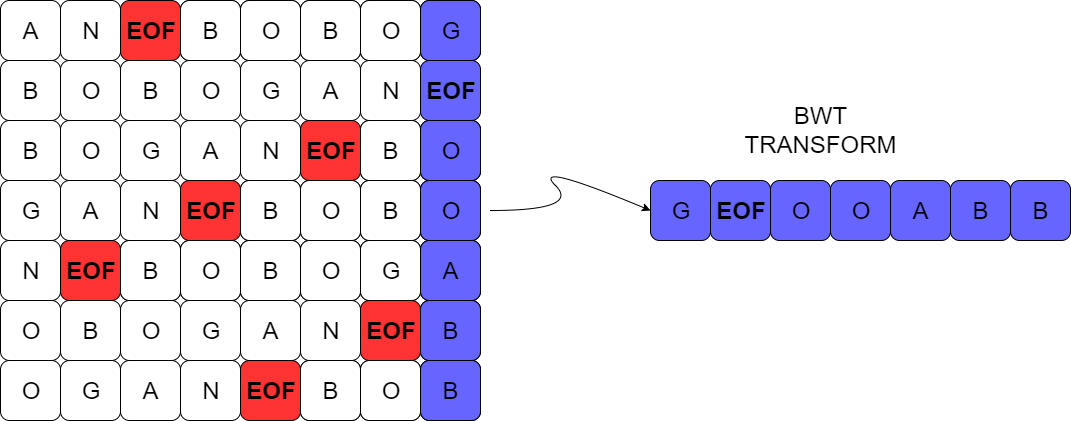
\includegraphics[width=1\textwidth]{pngOfDiagrams/bwtfinal.png}
\end{figure}

Therefore, for the string "BOBOGAN", the corresponding BWT would be "G*OOABB", where "*" is the character that denotes the end of the string. This idea of sorting the suffixes of the word seems familiar.

BWT is computed using suffix arrays. Using suffix arrays, the BWT compression is reduced to the following:

\begin{lstlisting}
void computeBWT(std::string s){
    std::vector<int> SA = suffixArray(s); // the suffix array of string "s", indexing starts at position 1
    for(int i = 1; i <= s.length(); ++i) // the last character is the ending character, and is the smallest lexicographic
        if(SA[i])
            cout << s[SA[i] - 1];
        else 
            std::cout << "$";
}
\end{lstlisting}

The time complexity is the same as computing the suffix arrays, $O(n \log ^ 2 n)$. For the transformation back to the original data, the inverse thought process is applied.


\newpage

\subsection{Levenshtein distance}

\paragraph{}

The Levenshtein distance (sometimes referred to  as "edit distance") between two strings is defined as the minimum number of single-character changes(deletion, insertion and substitution) required to transform a word such that it matches the second one. Browser engines use the Levenshtein distance in search suggestions. As a great example, if a miss-spell is detected by the search engine, then by using the Levenshtein distance against a database of common searches it can suggest the correct word, thus positively impacting the search result. 

Concretely, the defined operations for the Levenshtein distance are:

\begin{itemize}
    \item deletion: delete a character in the first string. As an example, if the string is "hello", a valid deletion of the first character would lead to the modified string "ello".
    \item insertion: insert a character at a desired position in the first string. As an example, if the string is "hello", a valid insertion would be "heello".
    \item substitution: substitute the $i$-th character of the first string with the $j$-th character of the second string. As an example, if the strings are "hello" and "goodbye", then a valid substitution would lead to the first string being modified as "yello".
\end{itemize}

As an example, the Levenshtein distance between the strings "aabc" and "abbca" is 2, and is reached by performing these operations:

\begin{figure} [h!]
\centering
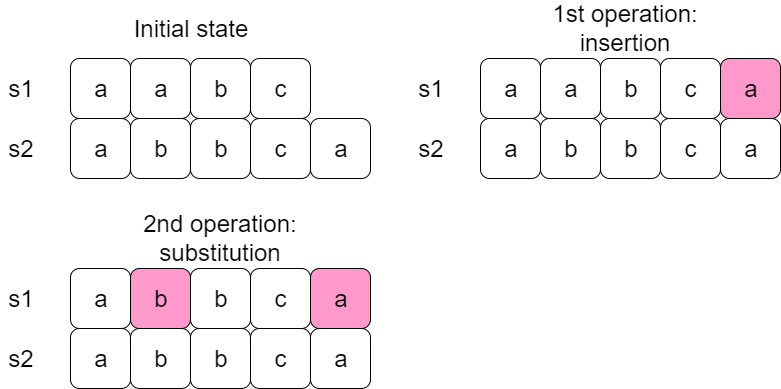
\includegraphics[width=1\textwidth]{pngOfDiagrams/levenshtein1.png}
\end{figure}

The algorithm that measures this metric is based on the technique of dynamic programming.  The algorithm makes use of a matrix to store intermediate results, and it works by filling in the elements of the array row by row, where each row corresponds to a prefix of one of the input strings.

The Levenshtein distance algorithm is based on the observation that any transformation of one string into another can be achieved by a sequence of single-character edits. Therefore, the problem can be solved by finding the minimum number of edits required to transform each prefix of one string into each prefix of the other string, and then using those results to compute the minimum number of edits required to transform the integral strings.

A matrix $DP$ will be instantiated. $DP_{ij}$ denotes the minimum edit distance between the first $i$ characters of the first string and the first $j$ characters of the second string. By using this definition, it is clear that $DP_{i0} = i$ and $DP_{0,j} = j$, since this is the amount of edits required to transform a prefix of one of the strings into the empty string.
For the other pair of prefixes $(i, j)$:

\begin{itemize}
    \item if the $i$-th character of the first string is equal to the $j$-th character of the second string, then $DP_{i + 1, j + 1} = DP_{ij}$
    \item otherwise, $DP_{i + 1, j + 1}$ is defined as the minumum of the following values:
    \begin{itemize}
        \item $DP_{ij} + 1$, denoting a substitution of the $i$-th character of the first string with the $j$-th character of the second string
        \item $DP_{i + 1, j} + 1$, denoting an insertion of the $j$-th character of the second string.
        \item $DP_{i, j + 1} + 1$, denoting a deletion of the $i$-th character of the first string
    \end{itemize}
    \item it is natural that the result is stored in $DP_{nm}$, which represents the minimum number of edits requires to transform the full first string into the full second string.
\end{itemize}

After the recurrence is built, the implementation becomes rather laconic:

\begin{lstlisting}
int levenshteinDistance(std::string &word1, std::string &word2) {
    int len1 = word1.length();
    int len2 = word2.length();

    int DP[len1+1][len2+1]; // DP[i][j] = minimum edit distance between first i chars of the first string and the first j chars of the second string

    for(int i=0; i<=len1; i++) {
        for(int j=0; j<=len2; j++) {
            if(i == 0) {
                DP[i][j] = j; // first line is computed
            }
            else if(j == 0) {
                DP[i][j] = i; // first column is computed
            }
            else if(word1[i-1] == word2[j-1]) { // in the case that the i-th character of the first string is equal to the j-th character of the second string
                DP[i][j] = DP[i-1][j-1];
            }
            else {
                DP[i][j] = 1 + min(DP[i][j-1], min(DP[i-1][j], DP[i-1][j-1]));
            }
        }
    }
    return DP[len1][len2];
}
\end{lstlisting}

The overall time complexity of the classic Levenshtein distance is $O(nm)$, where $n$ denotes the length of the first string and $m$ denotes the length of the second string. 

As discussed, the Levenshtein distance is very important in many fields that require to find lots of similarities between information. By using these concepts, a Levenshtein automaton can be build, that has the ability to recognise the set of all strings whose Levenshtein distance from $w$ is maximum $n$. The only limit to applying Levenshtein distance in real life is only the limitation that the human thought process can produce. 

\newpage

\section{Computational Geometry}

\subsection{The field of computational geometry}

\paragraph{}

The field of computational geometry is vast is considered to be a key component in many applications, ranging from basic collision detection to possibly 3D modelling. Computational geometry refers to a variety of algorithms related to geometry that benefit from the usage of high computing power. Computational geometry is used in interpreting and analysing huge input data formed of millions and millions of points, a good example would be the working principles of CAD(computer-assisted designing).

\begin{figure} [h!]
\centering
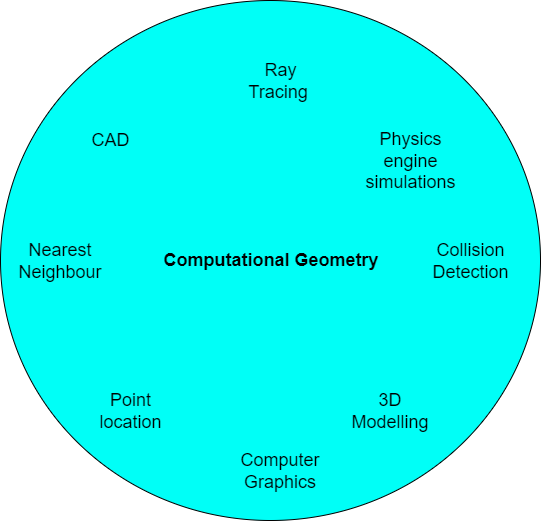
\includegraphics[width=0.67\textwidth]{pngOfDiagrams/thefieldofcomputationalgeometyr.png}
\end{figure}

Computational geometry serves as a foundation for key-concepts, such as discovering the nearest neighbour of an object in image processing, collision detection between different objects and ray-tracing, which is the technique of accurately simulating the lightning of a scene and its objects by rendering accurate reflections and refractions.

This chapter will serve as an appropriate introduction to multiple key-concepts and representative problems regarding this field. Another portion of this book will be dedicated to modelling computational geometry problems using the technique of "dynamic programming", which, in a way, changes the way of thinking about problems and introduces the reader to the very core or computer-science optimisations.

\newpage

\subsection{Closest pair of points}

As an introductory problem regarding advanced concepts in computational geometry, consider the following problem:

\begin{itemize}
    \item Given $n$ points in a Cartesian plane, compute the smallest possible distance between two points.
\end{itemize}

\begin{figure} [h!]
\centering
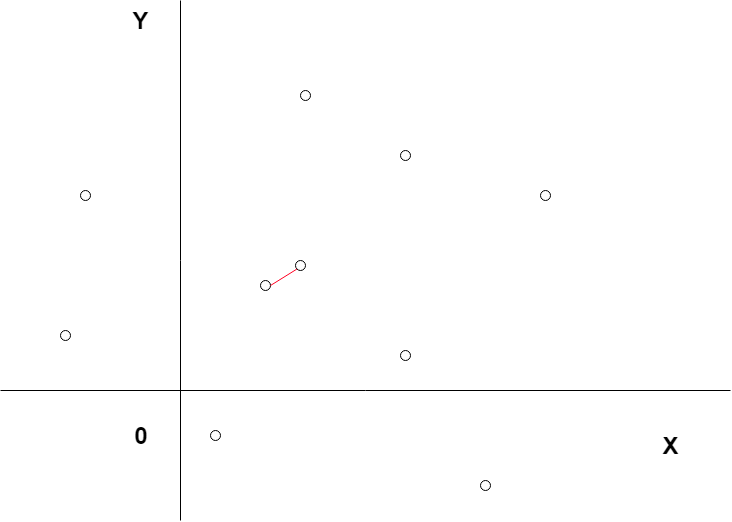
\includegraphics[width=0.85\textwidth]{pngOfDiagrams/closestpair1.png}
\end{figure}

This problem is very important in the field of possible collision detection and it can have many practical applications, such as preventing collision between cars or airplanes and designing different 3-dimensional technical objects, such as buildings and car parts.

At first notice, this problem seems trivial. A possible naive implementation would be selecting every distinct pair of points and computing the smallest distance between every one of them, remembering the best result. 

% descriere implementare naiva n2

In order to implement the naive approach, a point structure will be defined that will store the $x$ and $y$ values for each point. The distance between two points remains the classical: $d(a,b) = \sqrt{(x_a - x_b)^ 2 \cdot (y_a - y_b)^2}$.

\begin{lstlisting}
struct Point{
    double x,y;
};
const int NMAX = 100001;
Point P[NMAX];
double distance(Point a, Point b){
    return (double) sqrt((a.x - b.x) * (a.x - b.x) + (a.y - b.y) * (a.y - b.y));
}
\end{lstlisting}

In order to deal with points that contain negative value coordinates, all of the points will be translated to the positive side by addition with a constant factor(this does not impact the result).

%imaginea 2 este mai jos, nu este problema

\begin{figure} [h!]
\centering
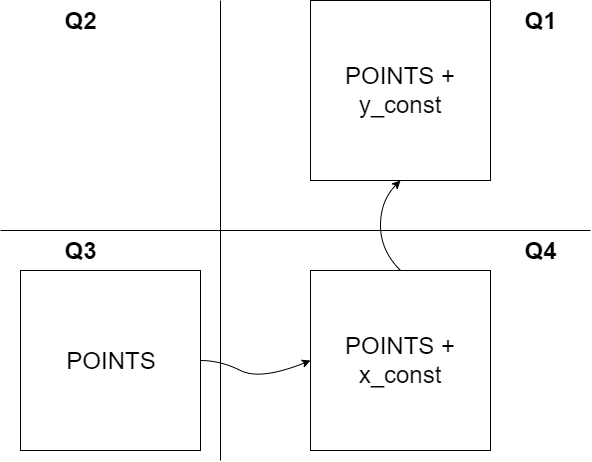
\includegraphics[width=0.75\textwidth]{pngOfDiagrams/closestpair3.png}
\end{figure}

\begin{lstlisting}
void shiftToPositive(int n){
    // if the n points have negative values, shift them so all of the coordinates are positive, this does not impact the result
    const double DISPLACEMENT = 1000.0;
    for(int i = 0; i < n; i++){
        P[i].x += DISPLACEMENT;
        P[i].y += DISPLACEMENT;
    }
}
\end{lstlisting}

For the final step, every pair of points is iterated through and the best result stored.

\begin{lstlisting}
double smallestDistance(){ // brute-force approach
    int n; // number of points
    std::cin >> n;
    for(int i = 0; i < n; ++i)
        std::cin >> P[i].x >> P[i].y;
    shiftToPositive(n);
    double bestDistance = 1000000.0;
    // checking every pair of points
    for(int i = 0; i < n - 1; ++i)
        for(int j = i + 1; j < n; ++j){
            double currDistance = distance(P[i], P[j]);
            if(currDistance < bestDistance)
                bestDistance = currDistance;
        }
    return bestDistance;
}
\end{lstlisting}

This implementation is not optimal, since it checks every possible pair of points in $O(n^2)$ time complexity. The time complexity can be reduced is the thought process is adapted and driven towards another implementation.

The solution is modelled using the concept "Divide et Impera" ("Divide and Conquer"). In the initial phase of the implementation, the points are sorted in ascending order according to the $x$ values. After the sort, the points are divided into two sets after the middle point. After this division, the closest pair of points in each half (denote it $d_1 and d_2$) is computed using a recursive approach.
 
\begin{figure} [h!]
\centering
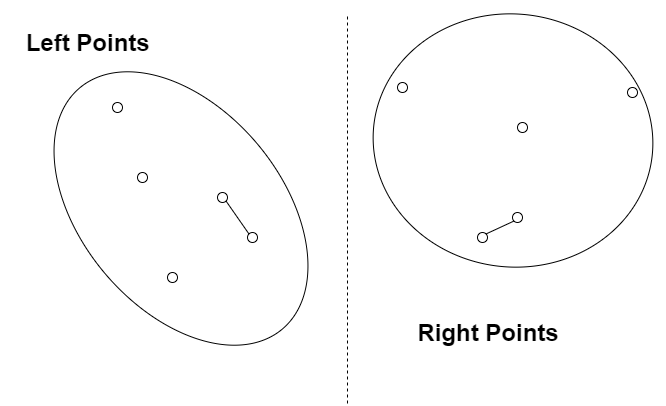
\includegraphics[width=0.85\textwidth]{pngOfDiagrams/closestpair2.png}
\end{figure}

This is not enough. What if the closest pair of points has a point that belongs in the first half and a point that belongs in the second half? A new corridor is created from the separation line that has the length on the both sided equal to the minimum distance between the already computed distances.

\newpage

\begin{figure} [h!]
\centering
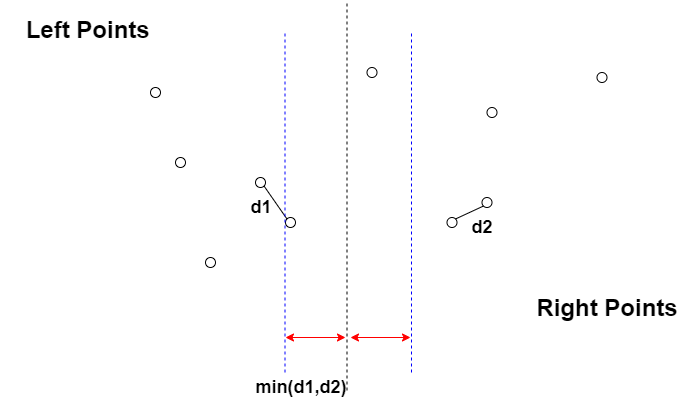
\includegraphics[width=1\textwidth]{pngOfDiagrams/closestpair4.png}
\end{figure}

All of the points that have the $x$ value closer to the dividing line that $min(d_1, d_2)$ are considered in the corridor. The values inside the defined corridor are sorted according to their $y$ coordinates, and then the smallest distance between them is computed. The result would be the minimum distance between the minimum distance found in the strip and the minimum distance found in the left and right brackets. Note that for a better time complexity, the points can also be sorted according to their $y$ values from the start (there is no need to sort the points in the corridor for each recursive call).

The first step is defining a function that, for a sorted by $y$ corridor computes the smallest distance between the points inside. Mathematically, the inner loop will never reach more than 7 iterations, so the time complexity is linear for this step.

\begin{lstlisting}
double closestDistanceonCorridor(Point corridor[], int N, double dist){
    // find the smallest distance in a corridor of length dist from the "dividing line" after the points are sorted according to Y
    // the inner loop won't iterate more than 6 times.
	double minimumDistance = dist; // Initialize the minimum distanceance as d
	for (int i = 0; i < N; ++i)
		for (int j = i+1; j < N && (corridor[j].y - corridor[i].y) < minimumDistance; ++j){
            double dd = distance(corridor[i],corridor[j]);
			if (dd < minimumDistance)
				minimumDistance = dd;
		}
	return minimumDistance;
} 
\end{lstlisting}

The next step is the phase of the Divide and Conquer approach. The classical approach contains two arrays that store the points sorted according to their $x$ and $y$ values, respectively. For the base case, if there are less than 3 points, then the smallest distance will be computed using the brute-force approach discussed earlier in the chapter.

\begin{lstlisting}
double DivideAndConquer(Point PX[], Point PY[], int n) {
    if (n <= 3)
        return brute(PX, n);
    // compute the middle point
    int mid = n / 2;
    Point middle = PX[mid];
    Point leftY[mid];
    Point rightY[n - mid];
    int left = 0, right = 0;
    for (int i = 0; i < n; i++) {
        if ((PY[i].x < middle.x || (PY[i].x == middle.x && PY[i].y < middle.y)) && left < mid)
            leftY[left++] = PY[i];
        else
            rightY[right++] = PY[i];
    }
    // "Divide et Impera Principle"
    double d1 = DivideAndConquer(PX, leftY, mid);
    double d2 = DivideAndConquer(PX + mid, rightY, n - mid);

    // Find the smaller of two distances
    double d = min(d1, d2);

    // initialise and build the corridor
    Point corridor[n];
    int j = 0;
    for (int i = 0; i < n; i++)
        if (abs(PY[i].x - middle.x) < d)
            corridor[j] = PY[i], j++;
    return closestDistanceonCorridor(corridor, j, d);
}
\end{lstlisting}

As a note, arrays can be sorted using a lambda function, instead of a "different criteria comparison" function. As a brief definition, a lambda function is an in-place, anonymous function that can be given as a parameter to the standard quick-sort function implemented in C++.

\begin{lstlisting}
double closestPairOfPoints(){
	Point PX[n], PY[n];
	for (int i = 0; i < n; i++){
		PX[i] = P[i];
		PY[i] = P[i];
	}
	sort(PX, PX + n, [&] (Point a, Point b) {return a.x > b.x});
	sort(PY, PY + n, [&] (Point a, Point b) {return a.y > b.y});
	return DivideAndConquer(PX, PY, n);
}
\end{lstlisting}

The time complexity of this approach is $O(n \log n)$, which is much better than the classical quadratic time that the brute-force approach provides.

It is interesting how many problems can be modeled using "out-of-the-box" principles. This is a remarkable introductory problem in the field of optimisations that are applied to geometry problems. Many more interesting problems will come that will push the boundaries of thought when regarding computational geometry.

\newpage

\subsection{Convex hull using Graham scans}

\newpage

\subsection{Dual space. Voronoi diagrams}

\paragraph{}

Analytical geometry problems can be modelled in a variety of ways that have the purpose of computing a task in the most efficient way possible. The need of a achieving a better time complexity has helped shape new representations of geometrical objects.

In order to organically discover the concepts, start from the following problem: given $n$ lines in a plane (all distinct) that do not pass through the origin, determine which of them are "visible" from the origin point. A line is visible from the origin point if it is not obstructed by another line.

\begin{figure} [h!]
\centering
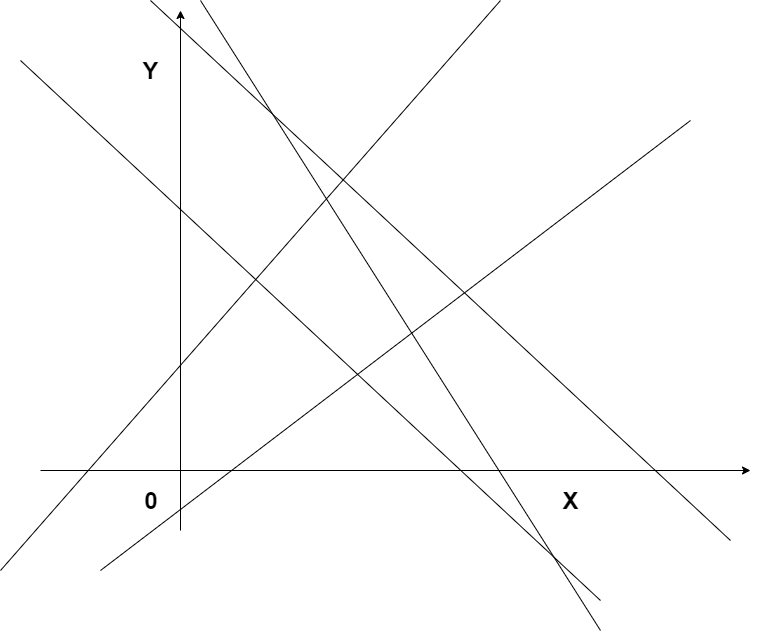
\includegraphics[width=1\textwidth]{pngOfDiagrams/dual1.png}
\end{figure}

This problem has many solutions. A not so elegant solutions runs in quadratic time. For every line $d_i$ the intersection with the other lines (denote it $d_j$) are computed. Consequently, $d_i$ is segmented into two semi-lines, for which only one is visible from the origin, the other one being shadowed by $d_j$. 

\newpage

\begin{figure} [h!]
\centering
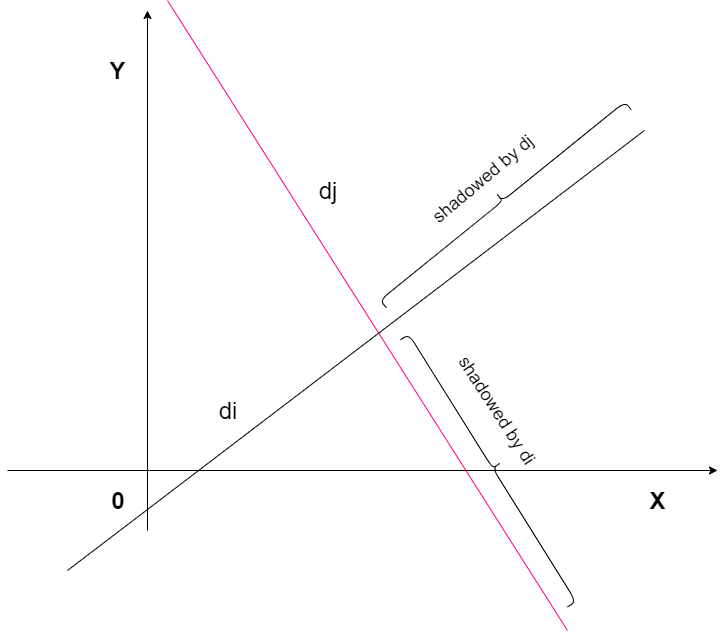
\includegraphics[width=0.85\textwidth]{pngOfDiagrams/dual2.png}
\end{figure}

At the end of computing the intersections and dividing the lines, a final check for a line visible from the origin point is made. This implementation has a $O(n^2)$ time complexity (due to iterating through every pair of lines) and it is not optimal to implement, since there are many edge cases (for example, perpendicular lines and parallel lines are considered edge cases).

There is however another concept that solves the problem in a better time complexity. From analytical geometry, a line is determined by the equation $Ax + By + c = 0$. From the initial hypothesis of the problem, the lines do not pass through the origin point, so $c \neq 0$. By diving with the $c$, we end up with another form of the line equation: $\frac{A}{c} + \frac{B}{c} + 1 = 0$. For simplicity, denote $\frac{A}{c} = a$ and $\frac{B}{c} = b$, so the notations are closer to the classical ones. The line equation becomes $ax + by + 1 = 0$.

Two new notions are defined: the primal space and the dual space. The "classical" lines are found in the primal space. On the other hand, the dual space is defined as the space that contains the points $(a,b)$ from the equation line definition of $ax + by + 1 = 0$. By using this thought process, every analytical geometry problem can be treated both in the primal and dual space. 

There are many relations between the primal and dual space that must be mentioned.

\begin{itemize}
    \item every line that does not pass through the origin point (since they cannot be divided by $c = 0$, therefore they are not defined in the dual space) in the primal space corresponds to a point in the dual space.
    
    \item every point in the dual space corresponds to a line in the primal space.

    \item what happens at an intersection between two lines in the primal space? Consider in the primal space $d1 = ax + by + 1 = 0$ and $d2 = tx + zy + 1 = 0$. Consider the intersection point $(u,v)$. The intersection point follows the rule: $au + bv + 1 = 0$ and $tu + zv + 1 = 0$. By dualising the lines, two distinct points are obtained: $p_1 = (a,b)$ and $p_2 = (t,z)$. In the dual plane, write the line equation that passes through said points: $\frac{x - a}{t - a} = \frac{y - b}{z - b}$. From the primal plane we know that $ax + by + 1 = tx + zy + 1$, consequently $(t - a)u + (z - b)v =0 $. By diving with $u \neq 0$, $(t - a) = - \frac{(z-b)v}{u}$. By using this result in the line equation for the points in the dual plane we can conclude that the line equation for $p_1$ and $p_2$ in the dual plane is $ux + wy + 1 = 0$.

    \item by dualising two points that determine a line in the primal plane we get two lines in the dual plane that intersect in a point.

    \item if, in the primal plane, $n$ lines intersect in a point $P$, in the dual plane would result co-linear points. 

\end{itemize}

\begin{figure} [h!]
\centering
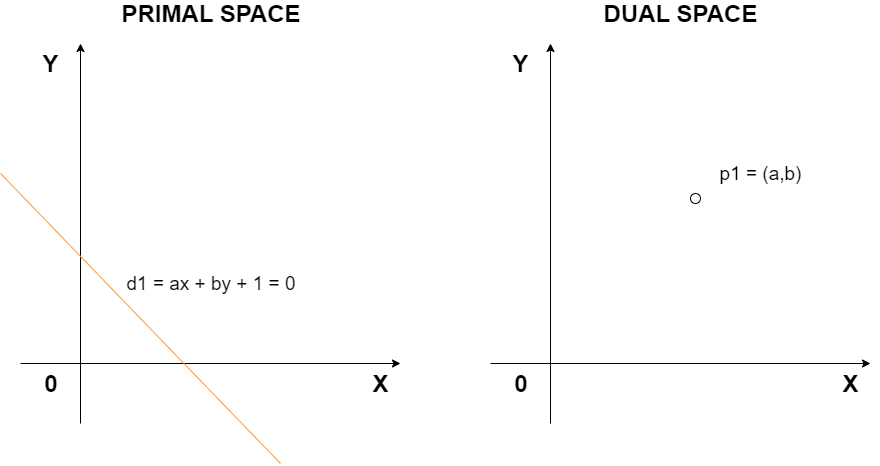
\includegraphics[width=1\textwidth]{pngOfDiagrams/dual3.png}
\end{figure}

Can we approach the initial introductory problem using this new theory? The answer is yes. Consider all of the initial lines. If all of the lines are dualised, then the points closer to the origin denote a line further line from the origin point and vice versa. Now the main problem is separating the visible lines from the "shadowed" lines. By using the dual space, it is natural that the lines that will be shadowed are the ones that are the furthest from the origin point (since other lines will be closer and will shadow them). This gives us the solution to the problem. 

In the construction of the solution, all of the lines in the primal space will be dualised. In order to find the lines in the primal space that are the closest to the origin, we need to find the points in the dual plane that are the furthest from the origin point. By computing the convex hull of the points in the dual plane, we find the respective closest lines from the origin in the primal space (since points situated on the convex hull in the dual plane are the farthest away from the origin).


\begin{figure} [h!]
\centering
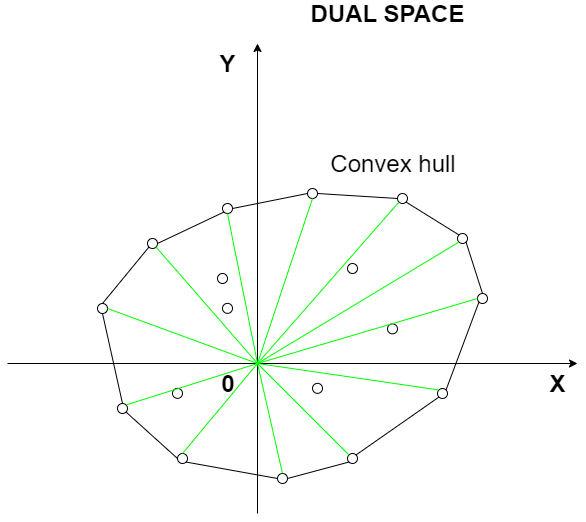
\includegraphics[width=0.7\textwidth]{pngOfDiagrams/dual4.png}
\end{figure}

Using the translation between the primal space and the dual space, this problem has an elegant solution that can be computed in $O(n \log n)$ time (the translation can be computed in linear time $O(n)$ and the convex hull is computed in $O(n \log n)$).

Translating the points from primal to dual is as easy as performing two divisions.

\begin{lstlisting}
struct Line{double a,b,c;};
struct Point{double x,y;};
int n; // number of lines of the form ax + by + c = 0
const int NMAX = 1000000;
Line lines[NMAX];
Point dual[NMAX];

void read(){
    std::cin >> n;
    for(int i = 0; i < n; ++i)
        std::cin >> lines[i].a >> lines[i].b >> lines[i].c;
}

Point primalToDual(Line &l){ // translates a line from primal space to a dual point
    l.a /= l.c;
    l.b /= l.c;
    l.c = 1;
    return {l.a, l.b};
}

void findVisibleLines(){
    for(int i = 0; i < n; ++i){
        Point p;
        p = primalToDual(lines[i]);
        dual[i] = p;
    }
    convexHull(dual, n);
}
\end{lstlisting}

After these notion were introduced, let's shift the topic to Voronoi diagrams.

Consider a convex polygon (for simplicity, consider a rectangle) and $n$ points inside it. The Voronoi polygon of a point $P_i$ is defined as the total number of points closer to $P_i$ than any other point $P_j$. The division of the convex polygon into multiple Voronoi polygons around a point is called a Voronoi diagram.

\begin{figure} [h!]
\centering
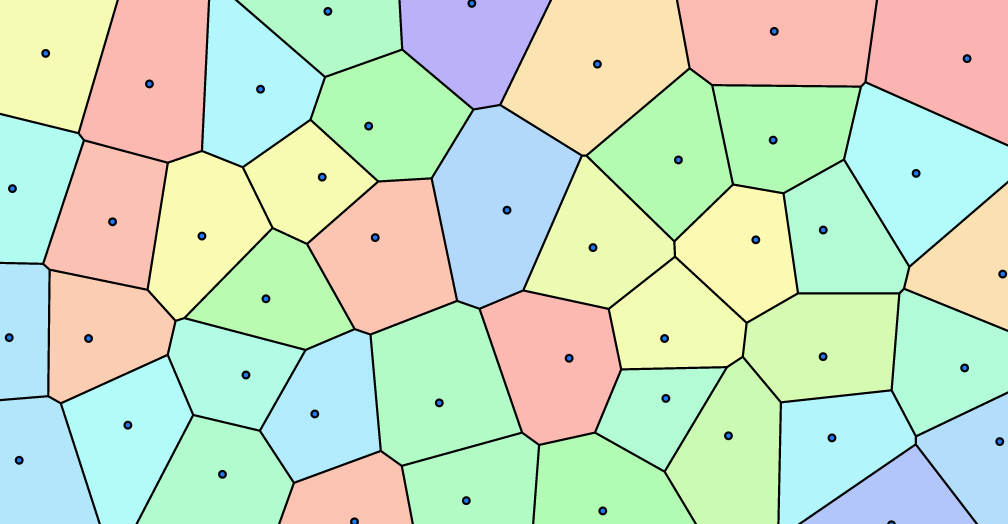
\includegraphics[width=1\textwidth]{pngOfDiagrams/voronoi2d1.png}
\end{figure}

The points on the diagram are also called "seeds". Starting from the base case, if there is only one seed, then the according Voronoi diagram is the starting polygon. 

If there are $n = 2$ seeds, denote them $A$ and $B$, then the construction logic is the following: construct the segment $AB$ and then construct its corresponding mediator. Intersect the mediator with the edges of the polygon and the Voronoi diagram is constructed. On the side of the mediator where the point $A$ is located are found all of the points closer to $A$, and on the side that $B$ is located in are found all of the points of the polygon that are closer to $B$. 

\newpage

\begin{figure} [h!]
\centering
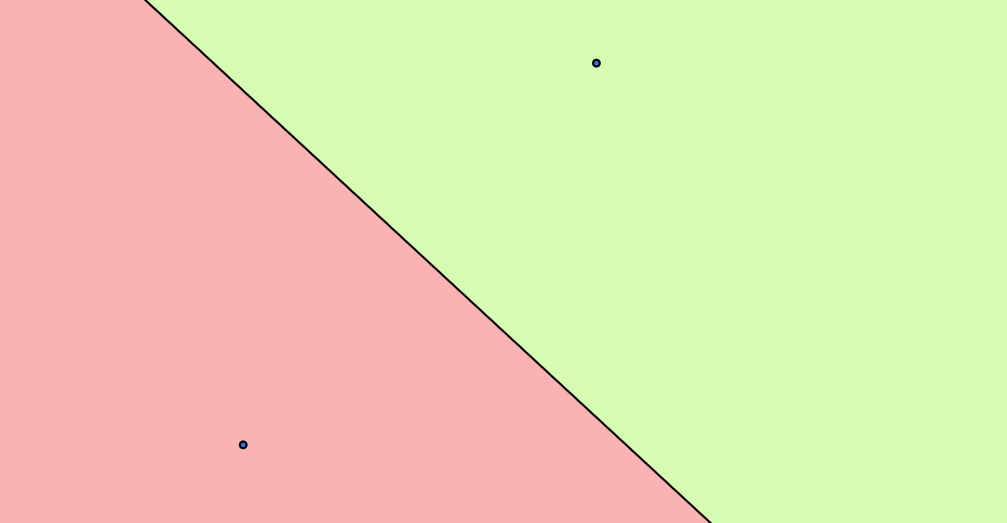
\includegraphics[width=1\textwidth]{pngOfDiagrams/voronoi2d2.png}
\end{figure}

In the case $n = 3$, denote the seeds $A$, $B$ and $C$, then the mediators of the segments $AB$, $AC$ and $BC$ are constructed. From the intersection point they are extended to intersect the polygon. The Voronoi diagram has been constructed.

\begin{figure} [h!]
\centering
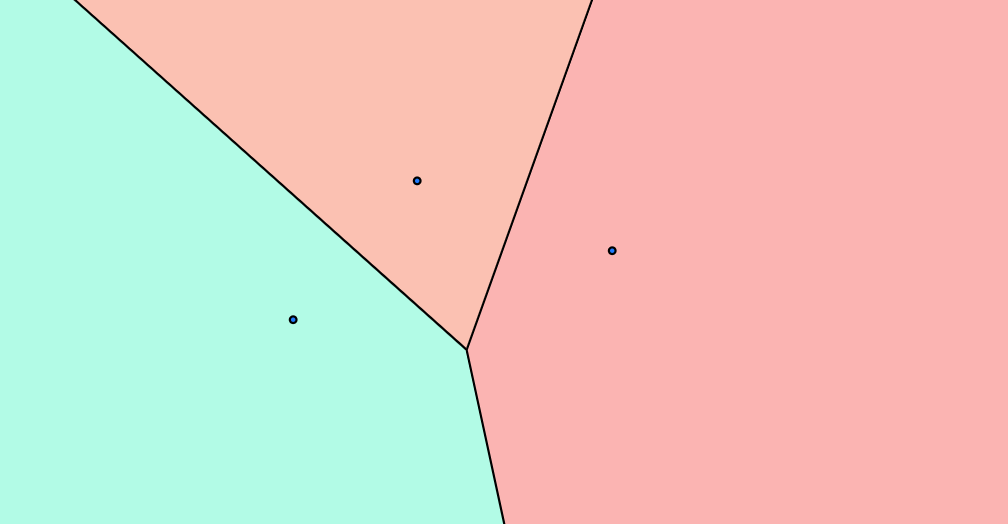
\includegraphics[width=1\textwidth]{pngOfDiagrams/voronoi2d3.png}
\end{figure}

The pattern can be seen for other values of $n$. A brute-force approach where the mediators of all pairs of points are computed is not efficient, since it would be computed in $O(n^3)$ time. 

By using the duality principle thought process,  for a point $P$, the Voronoi polygon would be delimited by the mediator lines that are "visible" from it. Consequently, the problem of constructing a Voronoi diagram for a set of points is reduced to the same introductory problem. In this case, however, for the duality principle to be applied, the origin point of the $X0Y$ coordinate system needs to be translated in order to coincide to the point that we want to compute the respective Voronoi polygon. 

\newpage

\begin{figure} [h!]
\centering
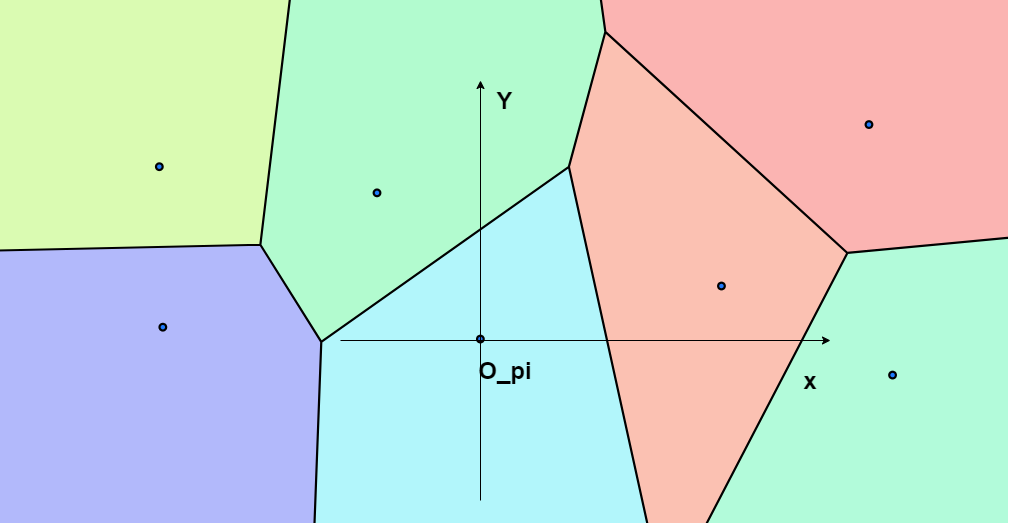
\includegraphics[width=1\textwidth]{pngOfDiagrams/voronoixoy.png}
\end{figure}

By using the dual space, we have managed to reduce the time complexity for computing a Voronoi diagram from $O(n^3)$ cubic time to $O(n^2 \log n)$ time, since for $n$ points we need to compute the convex hull in the dual space that takes $O(n \log n)$ time. This is an extraordinary example of a problem that can be solved by shifting from the primal space to the dual space.

Also interesting is the construction of a Voronoi diagram for a matrix (an image, for example). Since all of the coordinates are integer values, the breadth-first search (BFS) can be applied for every point. The BFS always guarantees the shortest distance, so it will compute the closest points to a fixed seed $P$. The problem is that there are multiple seeds. In this case, the multi-agent principle can used. The multi-agent principle refers to computing the shortest distance that an agent (in this case, a seed) can reach, without colliding with another agents on the path. This is excellent, since this follows the definition of the Voronoi diagram: the closest points to a seed belong in its respective Voronoi polygon. The multi-agent principle can be visualised pretty intuitively as a disease that spreads from one person to another in "layers" at the same time (in parallel).

\begin{figure} [h!]
\centering
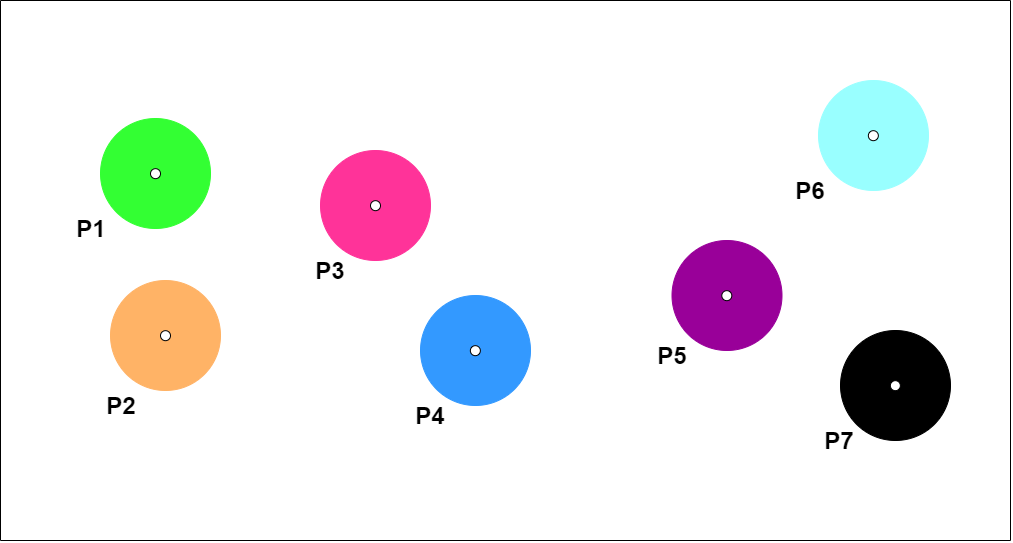
\includegraphics[width=0.75\textwidth]{pngOfDiagrams/voronoimulti.png}
\end{figure}

By running multi-agent BFS in a matrix until it is full should result in an "image" version of the Voronoi diagram. This can be computed in $O(nm)$, where $n$ denotes the number of lines and $m$ denotes the number of columns in the matrix.

\begin{lstlisting}
const int NMAX = 1000, MMAX = 1000; // dimensions of the matrix
const int dx[] = {-1, 0, 1, 0};
const int dy[] = {0, -1, 0, 1}; // direction vectors for 2D
int nSeeds;
stack<pair<int, int>> seeds;
int GRID[NMAX][MMAX];

void read(){
    std::cin >> nSeeds;
    for(int i = 0; i < nSeeds; ++i){
        int x,y;
        std::cin >> x >> y;
        seeds.push(make_pair(x,y));
    }
}

bool insideMatrix(int i, int j){
    return i >= 0 && i <= NMAX && j >= 0 && j <= MMAX;
}

void multiBFS(){
    queue<pair<int, int>> q; // standard queue implementation of the BFS
    int color = 0; // each color is parented to a point
    while(!seeds.empty()){ // planting the seeds in the grid
        q.push(make_pair(seeds.top().first, seeds.top().second));
        GRID[seeds.top().first][seeds.top().second] = ++color;
        seeds.pop(); 
    }
    while(!q.empty()){
        for(int d = 0; d < 4; d++){
            int iNew = dx[d] + q.front().first;
            int jNew = dy[d] + q.front().second;
            if(insideMatrix(iNew, jNew) && GRID[iNew][jNew] == 0){
                q.push(make_pair(iNew, jNew));
                GRID[iNew][jNew] = GRID[q.front().first][q.front().second]; // the neighboring seeds take the same color 
            }
        }
        q.pop();
    }

}

void printVoronoi(){ // prints the voronoi diagram
    for(int i = 0; i < NMAX; ++i){
        for(int j = 0; j < MMAX; ++j)
            std::cout << GRID[i][j] << ' ';
        std::cout << '\n';
    }
}
\end{lstlisting}

Voronoi diagrams have a lot of practical applications, ranging from applications in meteorology (by finding the weights of the precipitation data over an area), biology (studying the spread of a disease, fluid dynamics and simulations) and aviation (monitoring planes in order to avoid possible collisions).

Moreover, Voronoi diagrams can be extended to the three-dimensional space by modifying the previous implementation to account for the height of the new geometrical shape.

\begin{lstlisting}
const int NMAX = 100, MMAX = 100, HMAX = 100; //new dimension HMAX
const int dx[] = {-1, 0, 1, 0, ....};
const int dy[] = {0, -1, 0, 1, ....};
const int dh[] = {....}// direction vectors for 3D, length, width, height
int GRID[NMAX][MMAX][HMAX]; // the grid is now a 3D shape
\end{lstlisting}

By just a simple modification, beautiful 3D diagrams can be created, the only limit is the computational power of the rendering machine.

\begin{figure} [h!]
\centering
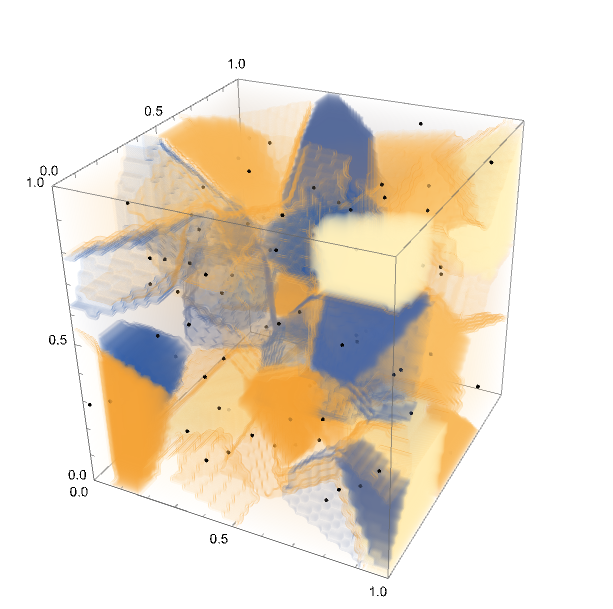
\includegraphics[width=0.75\textwidth]{pngOfDiagrams/voronoi3.png}
\end{figure}


\newpage

\subsection{The art gallery problem}

\newpage

\subsection{Water trap}

% \newpage

% \section{2SAT problem set}

\newpage

\section{Computational probabilities}

\paragraph{}

The realm of probabilities is a vast space which bends the mind and alters the conception about the nature of the events that may occur. By changing one small thing or one small probability in a series of events the future can be altered in such a manner that the new output is unrecognizable from the previous unaltered one. Consider the following examples: let's suppose that 100 distinct linear events exist. The goal is to calculate the probability of the last event occurring (the end-node event) based on the probabilities of the other 99 events in front of it that lead to it if they are met. The relations between the events can be visualised as such: 

\begin{figure} [h!]
\centering
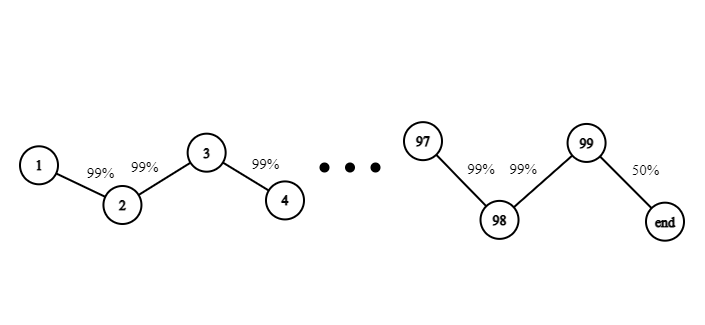
\includegraphics[width=0.91\textwidth]{pngOfDiagrams/slipperyslope.png}
\end{figure}

If all of the events leading up to the end-node event would have had the probability of $99\%$ of occurring, then the final event would've had the probability of "1 leading to 2 leading to $\dots$ leading to 100" is about $36\%$. If the last event had a probability of just $50\%$ of occurrence, then the result would have changed drastically, from $36\%$ ($0.99 ^ {99}$) to just $18\%$. This "falling domino: of probabilities show just how much a small change in the probability chain can alter the end-result and how hard it may be for a human to predict such output. This presented behaviour is known as "the slippery slope", where one series of domino-like occurrence of small events may cause a potentially unwanted end-event and it just shows how much a small change can lead to a different outcome.  

To see the mind-bending effect of probabilities, consider the following problem that stumbled 20th century mathematicians from around the globe. Suppose that you are on a game show and you are asked to choose between 3 doors. One door has a prize hidden behind it, and the other two doors don't. You make an initial selection. The host (which knows where the prize is hidden) opens a door that you have not chosen and shows you that there is no prize and asks you if you want to stick to your initial prediction or if you want to switch to another door. Should you make that switch?

\newpage

% pune imagine cu monty hall problem

\begin{figure} [h!]
\centering
\includegraphics[width=0.45\textwidth]{pngOfDiagrams/montyhall3.png}
\end{figure}

At first glance, it may seem that the contestant doesn't benefit from the switch as the probability of the other door apparently still remains the same ($33\%$), but the host showing the other door empty changes everything. Imagine the same scenario, but instead of 3 doors there are 100 doors. The contestant picks a random door. The host then opens 98 doors that do not contain the prize and leaves you with the same question: do you switch to the other door? Intuitively, now you should see the benefit of switching. If you mark the group of the other 99 doors that weren't picked with the probability of containing the prize of $99\%$, and then you remove from that group the 98 doors that don't contain the prize, the probability for the remaining one door is now the probability of the entire set, so the switch should definitely be made. 

% pune imagine cu monty hall 100

\begin{figure} [h!]
\centering
\includegraphics[width=0.87\textwidth]{pngOfDiagrams/montyhall100.png}
\end{figure}

These were just some basic examples to introduce the reader to the beauty of probabilities. This book will treat probabilities from the computer science perspective and will focus on the problems that can only be solved by computing the probabilities based on specific criteria and past predictions, from simple to complex.

\newpage

\subsection{Knight on a chess board}

\paragraph{}

A good warm-up problem in the field of probabilities sounds like this:

\begin{itemize}
    \item Given the initial positions for a knight on a generalized chess board, what is its probability of visiting a certain cell after exactly $k$ legal moves?
\end{itemize}

In order to solve this problem, let's use intuition to try and develop a solution from the base case to the more complex ones.

Firstly, it should be natural that the knight has a $100\%$ probability of being in the initial starting cell of the board. So at $k = 1$, the knight can only be found in the initial starting cell.

\begin{figure} [h!]
\centering
\includegraphics[width=0.51\textwidth]{pngOfDiagrams/knightone.png}
\end{figure}

At the next step ($k = 2$), it is logical that the knight would have a probability of landing in the 8 respective squares that it can legally land. Now the reader may ponder another good question. What is the respective probability that it may land in one of those cells? $\frac{1}{8}$, since there are $8$ possible positions that it can go to. In the next steps we will try to figure out a pattern that we can base an algorithm on.

\newpage

\begin{figure} [h!]
\centering
\includegraphics[width=0.51\textwidth]{pngOfDiagrams/knighttwo.png}
\end{figure}

However, at the next step, the pattern is not as easily recognisable. Let's try and simplify to one case. If the knight lands in a certain square, then the probability of him continuing its path from that selected square to another square would be the current probability of the knight landing in that respective square summed up with the current probability of the current position of the knight divided by the number of legal positions that it has(in our current case, 8). So we can consider the formula: 

$$p(square) = p(square) + \frac{p(prevSquare)}{8}$$

\begin{figure} [h!]
\centering
\includegraphics[width=0.51\textwidth]{pngOfDiagrams/kngihtthree.png}
\end{figure}

Now that the mechanism for just one knight is explained, now a pattern can already be seen that will lead to the correct solution and implementation of the problem.

\begin{figure} [h!]
\centering
\includegraphics[width=0.51\textwidth]{pngOfDiagrams/knightfour.png}
\end{figure}

As seen, this process needs to be repeated for every newly instantiated knight. In the diagram above, the red cells correspond to the second step, and the blue cells correspond to the third step and represent possible positions of the knight after $k$ moves. 

In order to construct a correct implementation, some key variables need to be instantiated.

\begin{lstlisting}
int n; // grid size
int istart, jstart, k;

bool pos[NMAX][NMAX]; // knights positions at step k 
int aux[NMAX][NMAX];
float ans[NMAX][NMAX]; // storing the result as a probability matrix 

// knight displacement vectors 

const int di[] = {-2, -1, 1, 2, 2, 1, -1, -2};
const int dj[] = {1, 2, 2, 1, -1, -2, -2, -1};
\end{lstlisting}

A function is needed in order to recreate the mechanism described above, let's call it $updatePos$, the argument being the current probability of the knight being found in the current cell.

\begin{lstlisting}
void read(){
    std :: cin >> istart >> jstart >> k >> n;
}

bool insideMatrix(int i, int j){
    // in chess indexing starts at 1
    return (i >= 1 && i <= n && j >= 1 && j <= n);
}

void updatePos(float currProb){
    // iterating through position matrix and updating auxiliary
    for(int i = 1; i <= n; ++i)
        for(int j = 1; j <= n; ++j){
            if(pos[i][j] == 1){ // a knight has been detected
                for(int pos = 0; pos < 8; ++pos){
                    // new fields for the knights
                    int lNew = i + di[pos];
                    int cNew = j + dj[pos];
                    if(insideMatrix[lNew][cNew]){
                        aux[lNew][cNew] = 1;
                        ans[lNew][cNew] += currProb / 8;
                    }
                }
            }
        }
    // copy the auxiliary matrix into the original
    for(int i = 1; i <= n; ++i)
        for(int j = 1; j <= n; ++j){
            pos[i][j] = aux[i][j];
            aux[i][j] = 0;
        }
}
\end{lstlisting}

Now that a mechanism has been constructed, it is time for it to be used in the main body of the program.

\begin{lstlisting}
void computeProbability(){
    float currProb = 1;
    ans[istart][jstart] = 1;
    pos[istart][jstart] = 1;
    for(int step = 1; step < k; step++){
        updatePos(currProb);
        currProb /= 8;
    }
}

void printResult(){
    std::cout << fixed << setprecision(3);
    for(int i = 1; i <= n; ++i){
        for(int j = 1; j <= n; ++j)
            std::cout << setw(8) << ans[i][j] << ' ';
        std::cout << '\n';
    }
}
\end{lstlisting}

There are many possible variations of these types of problems, but the concepts remain mostly the same. We hope that this problem serves as a great introduction of what's to come in the great field of computational probabilities.

\newpage

\subsection{Weather forecast}

\newpage

\subsection{Markov Chains}

\newpage

\subsection{Genetic algorithms. Modelling algorithms using a \\biological model}

\paragraph{}

Along the history of mankind, the strongest individuals that possessed the most balanced attributes have survived and prospered, contributing to a better society by adding value to it. The same can be said in modelling solutions to problems using genetic algorithms. At its core, genetic algorithms are based on randomly assigning attributes to individuals, evaluating them (which consists of assigning them an objective score) and preserving only the "elite players" among them. The same process can be found in real life, if we look at humanity history from its early beginning. Firstly, prehistoric humans can be viewed as the first generation of humans, which possessed a limited and very basic set of similar skills. Along the course of the human evolution, said people learned from others in order to survive, and the rest of them which were not able to adapt to the situation at hand perished. Therefore, we can say based on the theory of human evolution that individuals have adapted to the situation and "mutated" according to the specific environmental needs and the current problem that they were facing. Even now, society is evolving and changing constantly based on this theory and reality of evolution, so it is only natural that we ponder the question: "are we able to simulate something similar to natural and organic evolution of a specific input?"

At its core, genetic algorithms are a probabilistic method of solving NP-complete problems, where an end-state developed population of individuals can very easily describe the solution to a problem. The main goal of these types of algorithms is generating a bunch of naive solutions at first, evaluating them based on certain factors, separating and "killing" dumb individuals and repeating the process, by mutating only the best of the best individuals according to their specific score and reaching a very "intelligent population".

A very intuitive visualisation of a mutation can be represented as a string of DNA, where the green portions represent the attributes that remain the same and the red portions symbolise the genes that were changed in order to create a better population of individuals. 

\begin{figure} [h!]
\centering
\includegraphics[width=0.80\textwidth]{pngOfDiagrams/gene_mutation (1).png}
\caption{Mutation of genes visual analogy}
\end{figure}

\newpage

Using these ideas a person can construct different models that have various applications in real life, such as predicting the outcome of some actions based on previous evolution patterns that were observed. 

Remaining in the sphere of competitive programming, the usage of genetic algorithms can be very subtle but are a life-saver if used properly. In order to better understand the concepts that were presented, consider the following problem:

\begin{itemize}
    \item Given an array of integers, divide them into two sets such that the sum of these sets are as close as possible.
\end{itemize}

In order to visualise the core concept of dividing the integers into two distinct sets that have the most "similar" sums, consider the following example: if $v = \{ 17, 22, 35, 47, 49, 97, 85 \}, $ then the best way to separate those integers would be $set1 $ is denoted by $17+22+49+85 = 173$ and $set2$ is denoted by $ 35+47+97 = 179$. As seen, the sums that have resulted are as close as possible to one another, so the best division could be intuitively represented as the boolean array $[0, 0, 1, 1, 0, 1, 0]$, where $0$ and $1$ denote the two respective sets.

At first inspection, one may find different approaches to solving this task, either by brute-force or by computing the sum of an interval using different tricks such as prefix sums or data structures such as wavelet trees, but they are not as efficient or expandable (let's say that we want to divide the integers into 3 sets instead of just 2) as the method of simulating evolution. In the field of genetic algorithms, there are some steps that make the perfect recipe for success in a problem. 

Firstly, a good programmer must identify the type of problem that he is dealing with. A genetic algorithm problem can be recognised if the output can be described as the quality of a specific selection that may occur and many different possible outputs can be objectively evaluated and scored accordingly. In this problem, we can have many possible configurations of the output, but the absolute value of the sums in the two separate sets are way off the closest one, so their respective quality will be low.

After correctly classifying the problem, a good programmer must find a criteria which will be used in order to evaluate a score of an individual. In our case, the score that we assign to an individual would be the absolute difference between the sum of the integers in the first set and the sum of the integers in the second set. Note that many implementations can be valid in order to assign a score to an individual, so intuition and many experiments are key in determining the best way of evaluating a possible solution. As a general convention, a function that assigns a score to an individual is called a $fitness \ function$.

Using this approach, we will define some key variables related to genetic algorithms and these can be seen as an occurring theme in such problems.

\begin{lstlisting}
int n,v[NMAX]; // the array of integers
const int nGenerations = GEN; // arbitrary constant
const int nPopulation = POPULATION; // arbitrary constant
const int ELITE = nELITE;
struct Individual{int x[NMAX]; int score;};
vector <Individual> P; // a population at a given moment t
\end{lstlisting}

Some very important variables have been instantiated. The number of generations that we want to evaluate and the number of individuals in a population are 2 arbitrary constant integers that are carefully chosen in order to fit the needs of the problem. Here we need to strike a balance between $underfitting$ a genetic algorithm model (which will output a wrong result) and $overfitting$ (which will increase the number of computations needed in order to solve the problem). These concepts are very intuitive and based on real life dilemmas: should a company hire a small amount of people in order to solve a problem, risking that their respective experience may not be suitable for the job, or hiring a very large amount of people to work on said project, but risking of paying more wages than necessary. These concepts are also present in the field of $machine \ learning$, when dealing with large amount of data in order to train and fit a model. In our problem, and individual is defined as having a score and an array of boolean integers $x$, which will tell us if an element in the array $v$ is in the first or second set.

Now the modelling phase of the genetic solutions truly begins. At first, the initial population containing many individuals is created. Each individual is instantiated with random values of 0 and 1 and is scored according to a fitness function that matches the specifications of the problem described above.

\begin{lstlisting}
int fitness(Individual S){
    int sum1 = 0, sum2 = 0;
    for(int i = 1; i <= n; ++i){
        if(S.x[i] == 0)
            sum1 += v[i];
        else
            sum2 += v[i];
    }
    return abs(sum1 - sum2);
}
\end{lstlisting}

The population is the remembered and the individuals are sorted in the decreasing order of their scored. This ensures that at the start of the population array are the elite players of the generation that posses the best objectively attributed scores. For the next number of generations, an arbitrarily chosen number of elite players denoted $ELITE$ are copied and the new generation is modeled and mutated after them, and then the process of sorting them is repeated until the last generation. Therefore, it is obvious that the last generation contains only the best players and it is more likely to lead to the best result. The result is always stored in the best individual of the last generation.

\begin{lstlisting}
void read(){
    cin >> n;
    for(int i = 1; i <= n; ++i)
        cin >> v[i];
}

void geneticAlgo(){
    // as close to real random number generation
    srand(time(NULL)); 
    // initial population
    for(int k = 0; k < nPopulation; ++k){
        Individual S;
        for(int i = 1; i <= n; ++i)
            S.x[i] = rand() % 2;
        S.score = fitness(S);
        P.push_back(S);
    }
    sort(P.begin(), P.end(), [&] (Individual a, Individual b) {return a.score < b.score;});
    // more generations incoming
    for(int g = 1; g <= nGenerations; ++g){
        // new gen is obtained from P
        vector<Individual> newGen;
        for(int k = 0; k < ELITE; ++k) // number of elite players
            newGen.push_back(P[k]);
        for(int i = 0; i < nPopulation - ELITE; ++i){
            Individual S;
            S = P[i];
            int pos = rand() % n + 1;
            S.x[pos] = 1 - S.x[pos];
            S.score = fitness(S);
            newGen.push_back(S);
        }
        P = newGen;
        sort(P.begin(), P.end(), [&] (Individual a, Individual b) {return a.score < b.score;});

    }
}

void printResult(){
    for(int i = 1; i <= n; ++i)
        cout << P[0].x[i] << ' ';
}

\end{lstlisting}

As a very good exercise in understanding the basics of genetic algorithms, try and solve the same problem, but instead of dividing the initial array into 2 sets, try dividing them into 3. Can this model and implementation expand into possibly an $n$-set division of the array?

For problems that benefit from the use of genetic algorithms there is not a standard recipe for a correct implementation. In this initial problem, we represented an individual as having a boolean array, but there are many valid implementations when it comes to problem solving. Another ideas would be representing an individual as a permutation of different values from 1 to $n$, or as a transposition, depending on the respective problems. A good practice would be coming up with different solutions to the same problem, but representing the individuals using different means and comparing the results and the time complexity that has resulted in making the respective change. Furthermore, the selection of individuals can also be modelled using different ideas, such as random selection, roulette selection which makes use of the idea of calculating the sum of all scores and choosing an arbitrary number from 1 to the respective sum and choosing an individual accordingly to some specific criteria, elitism and other deviations from these enshrined methods.

\begin{figure} [h!]
\centering
\includegraphics[width=0.95\textwidth]{pngOfDiagrams/geneticalgo2dpiechart.png}
\caption{Roulette-wheel selection analogy}
\end{figure}

For example, the method of roulette selection can be visualised as such: imagine a casino table roulette-like game. Each individual has a sector of the respective table. Fitter individuals have a larger portion of the table than individuals that have not performed as well as them. The dealer throws a coin randomly on the table and the respective sector in which the coin has landed is marked, in our terminology, the said individual has been selected from the pool of possible candidates. Individuals that performed well and were assigned a good score are more likely to appear in the new population.

However, as far as current science is concerned, there are limitations to this method that can prevent solving increasingly complex tasks. The repeated use of the fitness evaluation function can spike up the time complexity considerably, consequently not being convenient for implementation. Moreover, in complex problems it can be very difficult to mix and match parameters in order to get the optimal result.

Genetic algorithms can also be used in many types of fields. Consider the following graph theory problem:

\begin{itemize}
    \item Given a graph, determine a maximum independent set(also called a "maximum stable component"). A maximum independent set is defined as a maximum set of nodes in a graph(directed or non-directed) such that no two nodes are connected.
\end{itemize}

Firstly, in order to solve the problem, it is good to understand the input and the concept of such maximum independent set. If the the given input is:

\begin{lstlisting}
7 8 (nodes and edges)
1 5
1 2
1 3
1 4
2 3
4 6
6 7
3 7
\end{lstlisting}

then the resulting graph:

\begin{figure} [h!]
\centering
\includegraphics[width=0.55\textwidth]{pngOfDiagrams/graphgenetic.png}
\end{figure}

The resulting graph would have the maximum independent set denoted by the outlined nodes. As an example, the nodes [2, 4, 5, 7] are not directly connected and form a maximum independent set of the respective given graph.

\newpage

\begin{figure} [h!]
\centering
\includegraphics[width=0.55\textwidth]{pngOfDiagrams/graphmaximumindependentset.png}
\end{figure}

Basic brute-force approaches are of no use in this problem, since they require too much calculations(for example computing the combinations between the nodes and then checking for a result). 

This problem can be solved using genetic algorithms and a special operation called "crossover" (or "recombination"). In crossover, an arbitrarily number of off-springs are produced using the genetic material of the parents.

% eventuale explicatii din cartea lui Mihai Oltean despre crossover

In order to implement this solution based of genetic algorithms, some definitions and declarations are necessary.

\begin{lstlisting}
int N; // nodes
int ADJ[101][101]; // adjacency matrix representation
int nrG = GEN; // arbitrary constant 
int nrP = POPULATION; // arbitrary constant

struct individ
{
    std::set <int> V;
    int fitness;
};

std::vector <individ> P;
\end{lstlisting}

The instructions are followed by key functions:

\begin{lstlisting}
void readInput(){
    std::cin >> N;
    for (int i = 1; i <= N; i++)
        for (int j = 1; j <= N; j++)
            ADJ[i][j] = 0;
    int M;
    std::cin >> M; //edges
    for (int i = 1; i <= M; i++){
        int a, b;
        std::cin >> a >> b;
        ADJ[a][b] = ADJ[b][a] = 1; 
    }
}

void mutation(individ &A){
    if (A.V.size() > 0){
        int pos;
        pos = rand() % A.V.size(); // specifying a random position
        std::set <int> ::iterator it;
        it = A.V.begin();
        for (int i = 1; i <= pos; i++)
            it++;
        A.V.erase(it);
        A.fitness--;
    }
    int peak;
    peak = rand() % N + 1; // random peak generation
    bool okay;
    okay = true;
    for (auto it: A.V)
        if (ADJ[it][peak] || it == peak) // checking for node connection
            okay = false;
    if (okay){
        A.V.insert(peak);
        A.fitness++; // assessing the fitness of an individual
    }
}

void crossover(individ A, individ B, individ &C, individ &D){
    C = A;
    for (auto itB: B.V)
        if (A.V.find(itB) == A.V.end()){
            bool okay;
            okay = true;
            for (auto itC: C.V)
                if (ADJ[itB][itC]){
                    okay = false; // violating the condition
                    break;
                }
            if (okay){
                C.V.insert(itB);
                C.fitness++;
            }
        }
    D = B; // repeating the process
    for (auto itA: A.V)
        if (B.V.find(itA) == B.V.end()){
            bool okay;
            okay = true;
            for (auto itD: D.V)
                if (ADJ[itA][itD]){
                    okay = false;
                    break;
                }
            if (okay){
                D.V.insert(itA);
                D.fitness++;
            }
        }
}

void printIndividual(individ &A){
    for (auto it: A.V)
        std::cout << it << " ";
}
\end{lstlisting}

Now that the concepts are implemented, the main body of the program that incorporates them is all that remains.

\begin{lstlisting}
void maximumIndependentSet(){
    srand(time(NULL));
    readInput();
    /// initialisation 
    for (int i = 1; i <= N; i++){
        individ A;
        A.V.insert(i);
        A.fitness = 1;
        P.push_back(A);
    }
    for (int i = N + 1; i <= nrP; i++){
        individ A;
        int peak;
        peak = rand() % N + 1;
        A.V.insert(peak);
        A.fitness = 1;
        P.push_back(A);
    }
    // sorting according to best fitness using lambda function
    sort(P.begin(), P.end(), [&] (individ A, individ B) {return A.fitness > B.fitness;}); 
    for (int g = 1; g <= nrG; g++){
        std::vector <individ> PNOU;
        /// elitism principle
        for (int i = 0; i < 5; i++)
            PNOU.push_back(P[i]);
        /// crossover steps
        for (int pas = 5; pas < nrP; pas++)
        {
            int ind1, ind2;
            ind1 = rand() % 5;
            ind2 = rand() % nrP;
            individ parent1, parent2;
            parent1 = P[ind1];
            parent2 = P[ind2];
            individ C, D;
            crossover(parent1, parent2, C, D);
            PNOU.push_back(C);
            PNOU.push_back(D);
        }
        /// mutation process
        int pos;
        pos = rand() % nrP;
        if (pos >= 5)
            mutation(PNOU[pos]);
        sort(PNOU.begin(), PNOU.end(), [&] (individ A, individ B) {return A.fitness > B.fitness;});
        P.clear();
        for (int i = 0; i < nrP; i++)
            P.push_back(PNOU[i]);
    }
    printIndividual(P[0]); // the result in stored in P[0]
    return 0;
}
\end{lstlisting}

Using this principle, a lot of problems can be viewed as a maximum internal set problem. Consider for example the N-Queen problem, where a player has to place the maximum amount of queens on a generalised chess board without them attacking each other. A graph can be constructed, mirroring the chess-board queen attack patterns, and then the whole problem is reduced to finding the maximum independent set of that constructed graph. 

\begin{itemize}
    \item Given a generalised $N \cdot N$ chess-board, compute the positions in which a player should place a maximum amount of queens such that no two queens attack each other.
\end{itemize}

Another concept that should be introduced: the number of generations drastically changes the output of the problem. In our test cases, 100 generations produced an unoptimised result and 200 generations produced the efficient placement of the queens.

As usual when coming to genetic algorithms, some declarations are needed:

\begin{lstlisting}
int N;
int ADJ[101][101];
int nrG = 100; // GEN, arbitrary choosen constant
int nrP = 200; // POPULATION, arbitrary choosen constant

struct individ
{
    set <int> V;
    int fitness;
};

vector <individ> P;
\end{lstlisting}

The graph needs to be construced from the generalised chess board based on the queen attack patterns:

\begin{lstlisting}
void initGraph() {
  int dim; // dimension of the chess board
  std::cin >> dim;
  ofstream fo("graf.out");
  N = dim * dim;
  fo << N << "\n";
  std::vector < pair < int, int > > EDGES;
  int M = 0;
  \\ graph construction respecting queen move patterns
  for (int l1 = 1; l1 <= dim; l1++)
    for (int c1 = 1; c1 <= dim; c1++)
      for (int l2 = 1; l2 <= dim; l2++)
        for (int c2 = 1; c2 <= dim; c2++)
          if (l1 != l2 || c1 != c2)
            if (l1 == l2 || c1 == c2 || abs(l1 - l2) == abs(c1 - c2)) {
              int v1, v2;
              v1 = (l1 - 1) * dim + c1;
              v2 = (l2 - 1) * dim + c2;
              if (v1 < v2) {
                M++;
                EDGES.push_back({
                  v1,
                  v2
                });
              }
            }
  fo << M << "\n";
  for (auto it: EDGES)
    fo << it.first << " " << it.second << "\n";
}
\end{lstlisting}

Then the resulting functions in order to prepare the main body of the program, mutation and crossover operations:

\begin{lstlisting}
void mutation(individ &A) {
  if (A.V.size() > 0) {
    int pos;
    pos = rand() % A.V.size();
    std::set <int> ::iterator it;
    it = A.V.begin();
    for (int i = 1; i <= pos; i++)
      it++;
    A.V.erase(it);
    A.fitness--;
  }
  int peak;
  peak = rand() % N + 1;
  bool okay;
  okay = true;
  for (auto it: A.V)
    if (ADJ[it][peak] || it == peak)
      okay = false;
  if (okay){
    A.V.insert(peak);
    A.fitness++;
  }
}

void crossover(individ A, individ B, individ & C, individ & D) {
  C = A;
  for (auto itB: B.V)
    if (A.V.find(itB) == A.V.end()) {
      bool okay;
      okay = true;
      for (auto itC: C.V)
        if (ADJ[itB][itC]) {
          okay = false;
          break;
        }
      if (okay)

      {
        C.V.insert(itB);
        C.fitness++;
      }
    }
  D = B;
  for (auto itA: A.V)
    if (B.V.find(itA) == B.V.end()) {
      bool okay;
      okay = true;
      for (auto itD: D.V)
        if (ADJ[itA][itD] == 1) {
          okay = false;
          break;
        }
      if (okay){
        D.V.insert(itA);
        D.fitness++;
      }
    }
}

void printResult(individ &A) {
  for (auto it: A.V)
    std::cout << it << " ";
}
\end{lstlisting}

An adaptation of the maximum independent set has been created for this problem. The remaining step is to place the queens on the chess board and evaluate the result that was obtained:

\begin{lstlisting}
void solve{
  srand(time(NULL));
  initGraph();
  readInput();
  /// init
  for (int i = 1; i <= N; i++) {
    individ A;
    A.V.insert(i);
    A.fitness = 1;
    P.push_back(A);
  }
  for (int i = N + 1; i <= nrP; i++) {
    individ A;
    int peak;
    peak = rand() % N + 1;
    A.V.insert(peak);
    A.fitness = 1;
    P.push_back(A);
  }
  sort(P.begin(), P.end(), [&] (individ A, individ B) {return A.fitness > B.fitness;});
  for (int g = 1; g <= nrG; g++) {
    vector < individ > PNOU;
    /// elitism concept, best of the generation remain
    for (int i = 0; i < 5; i++)
      PNOU.push_back(P[i]);
    /// crossover step
    for (int pas = 5; pas < nrP; pas++) {
      int ind1, ind2;
      ind1 = rand() % 5;
      ind2 = rand() % nrP;
      individ parent1, parent2;
      parent1 = P[ind1];
      parent2 = P[ind2];
      individ C, D;
      crossover(parent1, parent2, C, D);
      PNOU.push_back(C);
      PNOU.push_back(D);
    }
    /// mutation
    int pos;
    pos = rand() % nrP;
    if (pos >= 5)
      mutatie(PNOU[pos]);
    sort(PNOU.begin(), PNOU.end(), [&] (individ A, individ B) {return A.fitness > B.fitness;});
    P.clear();
    for (int i = 0; i < nrP; i++)
      P.push_back(PNOU[i]);
  }
  printResult(P[0]);
}

\end{lstlisting}

Note that from our testing, this implementation works best for values of $n \leq 5$. We leave as an exercise for the reader to implement a more efficient approach, pushing the boundaries of genetic algorithms optimisations.

As a final note, it is spectacular how many computer science concepts can be viewed and solved if genetic principles of evolution are applied correctly.

\newpage

\section{Sums, updates and queries}

\paragraph{}

This chapter of the book aims to introduce the reader to methods of computing certain actions(sums, maximums, etc.) in an efficient manner. Moreover, some of the structures that will be presented will support different operations that are defined on them, such as updates and queries in real time (the problem type is considered to be "online").

This book will start from the most elementary optimisations that can be made in regards to the topic and gradually expand the realm of efficient data structures.

\subsection{Prefix sums}

\paragraph{}

The most basic concept in regards to sum optimisations is sprung from the following problem:

\begin{itemize}
    \item Given an array $A$ of $n$ integers and $q$ queries of the form "what is the sum between the $x$-th element and the $y$-th element of the array?", output the respective answers to the queries. 
\end{itemize}

As an example, if $n = 8$, $A = [3, 5, 1, 9, 3, 1, 2, 8]$ and $q = 3$ queries of the form $[2, 5], [3, 4], [1, 8]$:

\begin{figure} [h!]
\centering
\includegraphics[width=0.77\textwidth]{pngOfDiagrams/prefixsum1.png}
\end{figure}

This problem seems trivial at first. The easiest way of solving this problem is iterating from position $x$ to position $y$ for every query.

\begin{lstlisting}
int n, q;
const int NMAX = 101;
int A[NMAX];

void naive(){
    std::cin >> n;
    for(int i = 1; i <= n; ++i)
        std::cin >> A[i];
    std::cin >> q;
    for(int i = 0; i < q; ++i){
        int x,y;
        std::cin >> x >> y;
        int s = 0;
        for(int i = x; i <= y; ++i)
            s += A[i];
        std::cout << s << ' ';
    }
}
\end{lstlisting}

This is a naive approach and it has a $O(Q \cdot N)$ time complexity, which is not good. A better solution would be constructing the prefix sums array for $A$. This concept is based on dynamic programming. The prefix sums array $DP$ will be built using the following recurrence: $DP_{i} = DP_{i - 1} + DP_{i}$, for $i = 1,\dots,n$.

\begin{figure} [h!]
\centering
\includegraphics[width=0.77\textwidth]{pngOfDiagrams/prefixsum2.png}
\end{figure}

This is a key observation, since now the sum for an interval $[x,y]$ can be computed in instant $O(1)$ time. The sum between $x$ and $y$ is the same as the difference $DP_{y} - DP_{x - 1}$. By definition, $DP_0 = 0$.

\begin{figure} [h!]
\centering
\includegraphics[width=0.77\textwidth]{pngOfDiagrams/prefixsum3.png}
\end{figure}

This method of computing the sums requires $O(n)$ linear time complexity in order to compute the $DP$ array.

\begin{lstlisting}
void prefixSums(){
    std::cin >> n;
    for(int i = 1; i <= n; ++i)
        std::cin >> A[i];
    for(int i = 1; i <= n; ++i)
        A[i] += A[i - 1]; // computing the DP array
    std::cin >> q;
    for(int i = 0; i < q; ++i){
        int x,y;
        std::cin >> x >> y;
        std::cout << A[y] - A[x - 1] << ' ';
    }
}
\end{lstlisting}

As practice for this introductory concept, consider the following problem:

\begin{itemize}
    \item An array with $n$ values , all equal to zero, exists. There are $q$ updates of the form $[x, y, val]$ with the signification: to all of the values between $x$ and $y$ is added value $val$. What does the final array look like?
\end{itemize}

Again, this problem can be solved in $O(Q \cdot N)$ using a brute-force approach. We can do better than that.

There is a very beautiful trick. For every update, on the position $x$ we add the value $val$ and on the position $y + 1$ we subtract the value $val$.

\begin{figure} [h!]
\centering
\includegraphics[width=0.7\textwidth]{pngOfDiagrams/prefixsum4.png}
\end{figure}

After all of the updates have been made, all that remains is computing the prefix sums array for $A$. This takes $O(n)$ linear time.

\begin{lstlisting}
void Mars(){
    std::cin >> n >> q;
    for(int i = 0; i < q; ++i){
        int x,y,val;
        std::cin >> x >> y >> val;
        A[x] += val;
        A[y + 1] -= val;
    }
    for(int i = 1; i <= n; ++i)
        A[i] += A[i - 1]; // computing the DP array
    for(int i = 1; i <= n; ++i)
        std::cout << A[i] << ' ';
}
\end{lstlisting}

The concept of prefix sums can be extended and applied for bi-dimensional arrays (matrices). The main concept remains the same, but the recurrence is changed in order to adapt to two dimensions. In order to compute the "prefix sums matrix", every element in the grid $A$ will follow this recurrence: $A_{ij} = A_{ij} + A_{i - 1, j} + A_{i, j - 1} - A_{i - 1, j - 1}$. This will efficiently compute the prefix sums matrix.

\newpage

\begin{figure} [h!]
\centering
\includegraphics[width=0.37\textwidth]{pngOfDiagrams/prefixmatrix.png}
\end{figure}

Once the prefix sums matrix has been computed in $O(nm)$, where $n$ denotes the number of lines and $m$ denotes the number of columns, calculating the sum of a sub-matrix can be calculated instantly by reversing the operators.

\begin{lstlisting}
void read(){ // reading the input
    std::cin >> n >> m;
    for (int i = 1; i <= n; i++)
        for (int j = 1; j <= m; j++)
            std::cin >> A[i][j];
}

void generatePartialSums(){ //  creating the prefix sum matrix using the recurrence (dynamic programming)
    for (int i = 1; i <= n; i++)
        for (int j = 1; j <= m; j++)
            A[i][j] += A[i - 1][j] + A[i][j - 1] - A[i - 1][j - 1];
}

long computeSubmatrixSum(int i, int j, int p, int q){ // computes the sum of a submatrix that starts at (i, j) and has the size (p, q)
    int i1 = i + p - 1;
    int j1 = j + q - 1;
    return A[i1][j1] - A[i1][j - 1] - A[i - 1][j1] + A[i - 1][j - 1]; // this is computed in O(1) time
}
\end{lstlisting}

\newpage

\subsection{Square root decomposition}

\paragraph{}

Square root decomposition is another method that answers queries for a given array $V$. The queries can vary depending on the type of the problem, but some of the most common queries regarding this data structure are: given two indices $l$ and $r$ ($l \leq r$), compute the sum/maximum/minimum for the interval determined by them. 

The entire idea revolves around separating the input into "buckets" (or blocks) of the same size, for which we know the answer to the query instantly using pre-calculations.

\begin{figure} [h!]
\centering
\includegraphics[width=1\textwidth]{pngOfDiagrams/sqrtdecomposition.png}
\end{figure}

Why is it important to divide the input into buckets when answering queries, for which we already computed the given answer(in this case, consider that we want to compute the sum for a given sub-array). The answer is simple: the sub-array that is given by the indices $l$ and $r$ may contain several buckets, consequently the time complexity will be reduced, since we do not need to compute again those respective sums. If one of the indices is placed inside of a bucket, then the individual terms remaining to reach another bucket would be added to the result "by hand" .This technique is often referred to as "data decomposition". 

\begin{figure} [h!]
\centering
\includegraphics[width=1\textwidth]{pngOfDiagrams/sqrtdecomposition2.png}
\end{figure}

For this particular example, if we need to compute the sum between $l = 2$ and $r = 11$, then it is convenient to only compute 4 summations: $V_2 + V_3 + S_2 + S_3$.

Now we need to solve another problem: what is the optimum size for the buckets? It is rather natural that if we divide the original array into very small buckets, then the number of calculations will be large, since we need to add up to the total sum a lot of the buckets.

\newpage

\begin{figure} [h!]
\centering
\includegraphics[width=1\textwidth]{pngOfDiagrams/sqrtdecomposition3.png}
\end{figure}

If the buckets are to small, then the answer will contain to many buckets additions. On the other hand, if the buckets are too large, then the problem is the exact opposite (to many individual terms need to be added to the total result).

\begin{figure} [h!]
\centering
\includegraphics[width=1\textwidth]{pngOfDiagrams/sqrtdecomposition4.png}
\end{figure}

In order to have a balance between the number of buckets and individual terms, the size of the buckets should be $\sqrt{n}$, where $n$ denotes the size of the initial array. If the square root contains decimals, it can be rounded up. If we use this process of thought, then the sum for a query $(l,r)$ should contain the smalles number of calculations. The time complexity of the square root decomposition is proportional to $O(\sqrt{n})$ for every query, since we need to traverse approximately $\sqrt{n}$ buckets, for which the result has already been computed in linear time.

\begin{figure} [h!]
\centering
\includegraphics[width=1\textwidth]{pngOfDiagrams/sqrtdecomposition5.png}
\end{figure}

This data structure also supports updates of the kind: for an index $i$, update the corresponding element with the value $x$. This process is very easy by updating the individual element in the initial array and updating the respective block.

Consider the following implementation of the square root decomposition, which is fitted for computing sums.

\begin{lstlisting}
const int NMAX = 1e5; // maximum number of elements
const int SQRTN = 320; // square root of NMAX
int n; // number of elements
int a[NMAX]; // the initial array
int b[SQRTN]; // the buckets
int blockSize; // the size of each block

int query(int l, int r){ // query the range (l, r) and return the sum
    long sum = 0;
    // if left belongs inside a bucket, add individual terms to the sum
    while (l % blockSize != 0 && l <= r) {
        sum += a[l];
        l++;
    }
    // if right belongs inside a bucket, add individual terms to the sum
    while (r % blockSize != blockSize - 1 && l <= r) {
        sum += a[r];
        r--;
    }
    // add the buckets to the sum
    while (l <= r) {
        sum += b[l / blockSize];
        l += blockSize;
    }
    return sum;
}

void update(int i, int x){ // update the element at index i to have the value x
    int block = i / blockSize; // find the corresponding bucket
    b[block] += x - a[i]; // update the bucket
    a[i] = x; // update in the initial array
}

void squareRootDecomposition(){
     // read the array
    std::cin >> n;
    for (int i = 0; i < n; i++) {
        std::cin >> a[i];
    }
    // precompute the blocks
    blockSize = sqrt(n);
    for (int i = 0; i < n; i += blockSize) {
        int sum = 0;
        for (int j = 0; j < blockSize && i + j < n; j++) {
            sum += a[i + j];
        }
        b[i / blockSize] = sum;
    }
    // answer queries and update elements
    int q;
    std::cin >> q;
    while (q--) {
        int type, l, r;
        std::cin >> type >> l >> r;
        if (type == 1) {
            std::cout << query(l, r) << '\n';
        } else {
            update(l, r);
        }
    }
}
\end{lstlisting}

This method can be rather powerful and it appears in many problems regarding different queries, such as the sum in an interval, the maximum/minimum element in an interval, the frequency of an element in an interval and so on. Depending on the type of query and update operations, in some practical problems and implementations, maybe it would be best to decompose the input into buckets of a different length than $\sqrt{n}$. By using this data structure and model, a good implementer needs to evaluate the correct block size in order to achieve the best time complexity and fit the respective needs of the task.

\newpage

\subsection{Fenwick trees}

\newpage

\subsection{2D Fenwick trees}

\newpage

\subsection{Segment trees}

\newpage

\section{Advanced dynamic programming model}

\subsection{Modelling a DP solution}

\paragraph{}

Dynamic programming (DP for short) represents a class of problems that can be solved by decomposing them into several sub-problems of the same type, that are generally much easier to compute and solve. The sub-problems may overlap, this constituting the main difference between DP and the technique "Divide et Impera". In the latter case, the sub-problems are completely separating. A common idea in DP modelling of a problem is finding a correct data structure to store the results for the sub-task, such as arrays or multidimensional structures where from they can be retrieved multiple times.

An individual may recognise a DP problem by its typical statements: "count the number of possibilities that satisfy respective conditions" and "find some maximum or minimum values for a respective input", but sometimes DP can be hidden and it may appear as a sub-problem itself.

\begin{figure} [h!]
\centering
\includegraphics[width=0.55\textwidth]{pngOfDiagrams/dpbasics.png}
\end{figure}


This chapter of the book aims to introduce the reader to advanced concepts regarding DP and aims to construct a general way of thinking about approaching such problems. Moreover, this chapter aims to teach the reader to see the hidden applications of DP and form a new way of thinking about the general concept of dividing the problem into more-easily computable sub-problems of a smaller scale.

\newpage

\subsection{DP meets chess}

\paragraph{}

In game theory, DP can be regarded as an important factor in solving a specific type of question: what is the number of ways that you can play the game when restrictions are introduced. Consider the following problem:

\begin{itemize}
    \item Suppose a board composed of $n$ lines, each line containing a certain number of equal squares. Line number $i$ contains $L_{i}$ squares and $L_{1} \leq L_{2} \leq L_{3} \leq \dots \leq L_{n}$. All the lines are aligned one beneath another and have the same place to begin. On this board we have to place exactly $k$ rooks such that there won't be two or more rooks that attack each other.
    
    What is the number of ways to do this action?
\end{itemize}

An example for $n = 5$ and $L_{1} = 1$, $L_{2} = 2$, $L_{3} = 3$, $L_{4} = 3$ and $L_{5} = 4$:

\begin{figure} [h!]
\centering
\includegraphics[width=0.40\textwidth]{pngOfDiagrams/dpchess1.png}
\end{figure}

Two rooks attack each other if they are on the same line or on the same column. Here is the same board and having $k = 3$ non-attacking rooks on it.

\begin{figure} [h!]
\centering
\includegraphics[width=0.35\textwidth]{pngOfDiagrams/dpchess2.png}
\end{figure}

For the approach, denote $R_{ij}$ the number of possibilities to place exactly $j$ rooks on the first $i$ lines of the board such that there aren't two or more rooks that attack each other. If we manage to compute the matrix R, then the answer to the problem will obviously be $R_{nk}$. According to the definition, we have the following relation between the elements of $R$:

\begin{itemize}
    \item $R_{ij} = R_{i - 1}{j} + R_{i - 1 j - 1} \cdot (L_{i} - (j - 1))$

    This takes into account the two possibilities that we have:

    \item there won't be any rook on the i'th line and we have to place the $j$ rooks among the first $i - 1$ lines
    \item there will be exactly one rook on the line $i$ and there are $L_{i} - (j - 1)$ possibilities to place it ($j - 1$ rooks will be placed on the first $i - 1$ lines and each of them restricts one column to be used by the current rook).
\end{itemize}

\begin{figure} [h!]
\centering
\includegraphics[width=0.35\textwidth]{pngOfDiagrams/dpchess3.png}
\end{figure}

There is however and edge case: $R_{i0} = 1$ (there is exactly one possibility to place zero rooks, regardless of the size of the board).

\begin{itemize}
    \item due to the fact that each element from the line $i$ in $R$ depends on elements situated in the line $i - 1$, all the operations can be organised such that instead the matrix $R$ we use only two arrays. However, using a matrix can make the solution easier to understand
    \item large values can be obtained in $R$ even for small values of $n$ and $k$(in that case the implementation of BigInteger operations might be a good idea).
\end{itemize}

Once the thought process of the DP is completed, the implementation is rather laconic.

\begin{lstlisting}
const int NMAX = 101;
int n,k;
int L[NMAX];
long long R[NMAX][NMAX];

void readInput(){
    std::cin >> n >> k;
    for(int i = 1; i <= n; ++i)
        std::cin >> L[i];
}

void DP(){
    for(int i = 0; i <= n; ++i)
        R[i][0] = 1; // edge case
    for(int i = 1; i <= n; ++i)
        for(int j = 1; j <= k; ++j)
            R[i][j] = R[i - 1][j] + (L[i] - (j - 1)) * R[i - 1][j - 1]; // construction of the DP matrix
    std::cout << R[n][k]; // result 
}
\end{lstlisting}

Now that the DP warm-up has ended, consider the following problem:

\begin{itemize}
    \item Suppose a chess board composed of $n$ lines, each line contains $n$ equals squares. The task is to count the number of possibilities to place $k$ bishops on it such that no two bishops attack each other. Two bishops attack each other if they are on the same diagonal.
\end{itemize}

In this figure is illustrated one of the possible solutions for the case $n = 4$ and $k = 3$.

\begin{figure} [h!]
\centering
\includegraphics[width=0.40\textwidth]{pngOfDiagrams/dpchessbishop1.png}
\end{figure}

This problem has a very elegant solution and it is great because it teaches the reader a new way of thinking about approaches in general. What is the main difference between this problem and the one with the rooks? Now the bishops move diagonally. So, what if instead of solving a new problem for the bishops, we transform the entire problem? What happens if we rotate the board $\frac{\pi}{4}$ radians clockwise?

\newpage

\begin{figure} [h!]
\centering
\includegraphics[width=0.55\textwidth]{pngOfDiagrams/bihsop3.png}
\end{figure}

Now the problem is the same, but the bishops now move vertically instead of horizontally, much like the rooks! Now the only problem remaining is correctly transposing the rotated chess board into a normal chess board, then the problem is reduced to the first problem presented.

The first idea would be separating the white squares of the board from the others, since two bishops can attack each other if and only if they are situated on squares of the same color.

\begin{figure} [h!]
\centering
\includegraphics[width=0.95\textwidth]{pngOfDiagrams/dpchessboardseparation1.png}
\end{figure}

The next step is rearranging the boards to look "normally".

\newpage

\begin{figure} [h!]
\centering
\includegraphics[width=0.87\textwidth]{pngOfDiagrams/dpchessboardseparation2.png}
\end{figure}

Now the problem is translated to trying all the possibilities to put $p$ non-attacking rooks on the board from the left and the remaining $q = k - p$ rooks on the board from the right that are also non-attacking.

As a final step, if we rearrange the lines in both two boards, in increasing order of their lengths, the result remains the same. This operation does not change the number of possibilities to put non-attacking rooks on the board.

\begin{figure} [h!]
\centering
\includegraphics[width=0.80\textwidth]{pngOfDiagrams/dpchessboardseparation3.png}
\end{figure}

Finally, we have succeeded to translate the problem into the introductory simpler DP problem, using clever thinking and imagination.


\newpage

\subsection{Games, paths and 3-dimensional DP}

\paragraph{}

DP can be used in solving a different variety of problems, ranging from games to solving different optimisation-related problems regarding paths. Modelling such problem using DP can be regarded as the practice of computing smaller sub-tasks and generating new results based on the previous answers by respecting the rules of the game in the process.

As a classic introductory problem, consider the following statement:

\begin{itemize}
    \item "IOI 1996": Consider a following two-player game. The game consists of a sequence $n$ positive integers, $X$. The two players move alternatively.

    When a player moves he selects a number from either left or the right end of the sequence $X$. The selected number is removed. The game is over when all of the numbers have been eliminated.

    Let $S_A$ be the sum of the numbers selected by the first player and $S_B$ be the sum of the numbers selected by the second player.

    The task is to find a winning strategy for the first player in two different cases:
    \begin{itemize}
        \item $n$ is even
        \item $n$ is odd
    \end{itemize}
\end{itemize}

For a visualisation of the problem, suppose the next example where $n = 8$:

\begin{figure} [h!]
\centering
\includegraphics[width=0.90\textwidth]{pngOfDiagrams/gamesandpaths1.png}
\end{figure}

The first player, $A$ has to choose between the leftmost and the rightmost values(3 and 2) in this particular case. Let's suppose he chooses 3. The new board is:

\begin{figure} [h!]
\centering
\includegraphics[width=0.90\textwidth]{pngOfDiagrams/gamesandpaths2.png}
\end{figure}

The second player, $B$, needs to choose now between the leftmost and the rightmost values(10 and 2). Let's suppose he chooses 10. A possible evolution of the game leads to $S_A = 3 + 8 + 7 + 15 = 33$ and $S_B = 10 + 9 + 3 + 2 = 24$. In this case, the first player wins the game.

\newpage

\begin{figure} [h!]
\centering
\includegraphics[width=1\textwidth]{pngOfDiagrams/gamesandpaths3.png}
\end{figure}

If $n$ is even, then a clever observation shows that the first player has a winning strategy, regardless of the values in $X$. Let's calculate the two sums, $S_1$ and $S_2$. $S_1$ denotes the sum of the values situated on odd positions and $S_2$ denotes the sum of the values situated on even positions in $X$.

\begin{figure} [h!]
\centering
\includegraphics[width=0.90\textwidth]{pngOfDiagrams/gamesandpaths4 (1).png}
\end{figure}

The first player, $A$, compares $S_1$ and $S_2$ and takes advantage of the fact that he is the first to move. If $S_1 \geq S_2$ then he will select $X_1$, otherwise, he will select $X_n$. When the second player, $B$, must perform his move, he, apparently, can change the course of the game but, in reality the first player can lead the game in such manner that he selects the numbers that form the greater sum among $S_1$ and $S_2$.

If $n$ is odd the same strategy does not work. In this case, a solution based on DP can provide the best result that player $A$ can obtain. In this case:

\begin{itemize}
    \item Denote $DP_{ij}$ the maximum difference that can occur between $S_A$ and $S_B$ if the game takes place on the fragment of the board composed of $X_i, X_{i + 1}, \dots, X_j$.
    \item If $DP_{1n} \geq 0$, then the first player has a winning strategy.
    The starting values in $DP$ are $DP_{ii} = X_i$, for $i = 1,2,\dots ,n$.
    \item It can be concluded that $DP_{ij} = max(X_i - DP_{i + 1, j}, X_j - DP_{i, j - 1})$.
\end{itemize}

After these notations, the implementation is rather laconic.

\begin{lstlisting}
int n, X[NMAX], DP[NMAX][NMAX];

void solve(){
    std::cin >> n;
    for(int i = 1; i <= n; ++i){
        std::cin >> X[i];
        DP[i][i] = X[i];
    }
    for(int i = n - 1; i >= 1; --i)
        for(int j = i + 1; j <= n; ++j)
            DP[i][j] = std::max(X[i] - DP[i + 1][j], X[j] - DP[i][j - 1]);
    if(DP[1][n] >= 0)
        std::cout << "Player A has a winning strategy!";
    else
        std::cout << "Player A has no winning strategy!";
}

\end{lstlisting}

Upping the difficulty, consider the following problem:

\begin{itemize}
    \item "The path with the maximum score in a grid": A matrix , $V$, with $n$ lines and $m$ columns and containing integer values is given. What is the maximum sum someone can obtain on paths that start in the top-left corner of $V$ and end in the bottom-right corner of said matrix? The paths we consider are not allowed to go go outside $V$ and always go one square to the right or downward from the current position.
\end{itemize}

\begin{figure} [h!]
\centering
\includegraphics[width=0.43\textwidth]{pngOfDiagrams/gamesandpaths5.png}
\end{figure}

As the solution, a second matrix, $W$ is constructed.

\begin{itemize}
    \item $W_{ij}$ denotes the sum for the best path from $(i, j)$ to $(n,m )$.

    \item $W_{ni} = V_{ni} + W_{n, i + 1}$, for $i = m - 1, \dots, 1$.

    \item $W_{im} = V_{im} + W_{i + 1, m}$, for $i = n - 1, \dots, 1$.

    \item $W_{ij} = V_{ij} + max(W_{i + 1, j}, W_{i, j + 1})$.

    \item Consequently, the answer will be stored in $W_{1,1}$.
\end{itemize}

Using this recurrence, for the given example the auxiliary matrix $W$:

\begin{figure} [h!]
\centering
\includegraphics[width=0.43\textwidth]{pngOfDiagrams/gamesandpaths6.png}
\end{figure}

\newpage

Twisting this problem, consider the following statement:

\begin{itemize}
    \item "A slightly different maximum path problem": Suppose we have to find the maximum sum for a path from $(1,1) to (n,m)$ in a matrix $V$ that contains positive integers values and the moves we can perform are one square up, down, to the left or to the right from the current position.
\end{itemize}

\begin{figure} [h!]
\centering
\includegraphics[width=0.43\textwidth]{pngOfDiagrams/gamesandpaths7.png}
\end{figure}

This problem is unique because it teaches a new way of thinking. The solution can be constructed based on the following observations:

\begin{itemize}
    \item If among $n$ and $m$ at least one is odd then we can easily find a path that goes over all the elements in $V$. For example, if $n$ is odd then the elements of $V$ in the first line are visited from left to right, the second line from right to left and so on for the other remaining lines.

    \item If both $n$ and $m$ are even, then we paint the elements of $V$ alternatively, like on a chess board. The upper-left and bottom-right squares are of the same color and it is not possible to find a path that contains all of the squares of the matrix $V$,
\end{itemize}

\begin{figure} [h!]
\centering
\includegraphics[width=0.43\textwidth]{pngOfDiagrams/gamesandpaths8.png}
\end{figure}

\begin{itemize}
    \item If $n$ and $m$ are even then it is not possible to find a path that visits each square exactly once. One of the purple squares cannot be visited.

    \item So, which of the dark orange squares we must avoid? Obviously, to obtain a maximum sum, we have to avoid the purple square with the minimum value.

    \item Not another question rises: is it possible to find a path from $(1,1)$ to $(n,m)$ that avoids any purple square? The answer is a firm "Yes". The matrix is divided into horizontal strips of width 2. The strips above that one which contains the avoided square are "swept" from left to right and after that form right to left(horizontally).
    The strip that contains the avoided square are "swept" vertically. The strips below that one which contains the avoided square are "swept" horizontally, again.

\end{itemize}

\begin{figure} [h!]
\centering
\includegraphics[width=0.8\textwidth]{pngOfDiagrams/gamesandpaths9.png}
\end{figure}

For the next example of a problem, DP meets sets.

\begin{itemize}
    \item "The dainty princess, National Olympiad in Informatics Romania": A dainty princess from the realm of Transylvania wants to marry and she has $n$ suitors. They form a line and each of them has a certain number of diamonds he wants to give to the princess. Suppose that the suitor $i$ has $D_i$ diamonds.

    But, while the suitors wait to meet the princess, they can negotiate their chances. More exactly, two neighbouring suitors, $i$ and $i + 1$ can make a deal: if $D_i \geq D_{i + 1}$ then the suitor $i$ can give $D_{i + 1}$ diamonds to the suitor $i + 1$, who leaves the line and abandons his plans to marry the princess(but at least he gains some diamonds in return). Otherwise, the suitor $i + 1$ can give $D_i$ diamonds to suitor $i$ to leave the line.

    The task is to determine the number of diamonds the last remaining suitor can have when he meets the dainty princess.
\end{itemize}

As an example, suppose $n = 6$ and $D$ contains $[3,4,5,6,1,3]$. Suppose that the suitor 4 "pays" the suitor 3 to leave the line. The new array $D$ is $[3,4,1,1,3]$. Suppose that the suitor 2 pays the suitor 3 to go home. The new array is $[3,3,1,3]$. Suppose that suitor 1 pays the suitor 2 to give up his marital plans. The new array $D$ becomes $[0, 1,3]$. Suppose that suitor 2 gives 0 diamonds to the first suitor to vanish. The new array is $[1,3]$. Now, the second suitor gives 1 diamond to suitor 1 and wishes him "good luck". The last suitor now has 2 diamonds to offer to the dainty princess.

For the solution, consider the following principles:

\begin{itemize}
    \item As usual, a matrix $DP$ with $n$ lines and $n$ columns will be built.

    \item $DP_{ij}$ contains a set of numbers(diamonds that the last suitor selected from the suitor from $i$ to $j$ can have).

    \item $DP_{ij}$ is obtained from all the possible values $DP_{i,k}$ combined with $DP_{k + 1, j}$.

    \item The answer to the problem will be stores in $DP_{1, n}$.
\end{itemize}


\begin{figure} [h!]
\centering
\includegraphics[width=1\textwidth]{pngOfDiagrams/dairyprincess.png}
\end{figure}


\begin{lstlisting}
const int NMAX = 51;
int n, D[NMAX];
std::set<int> DP[NMAX][NMAX];

void solve(){
    std::cin >> n;
    for(int i = 1; i <= n; ++i)
        std::cin >> D[i];
    for(int i = 1; i <= n; ++i)
        DP[i][i].insert(D[i]);
    for(int i = n - 1; i >= 1; --i)
        for(int j = i + 1; j <= n; ++j){
            // DP[i][j] is obtained
            for(int k = i; k <= j - 1; ++k)
                for(auto it1 : DP[i][k])
                    for(auto it2 : DP[k + 1][j])
                        if(it1 >= it2)
                            DP[i][j].insert(it1 - it2);
                        else
                            DP[i][j].insert(it2 - it1);
        }
    for(auto it : DP[1][n])
        std::cout << it << ' ';
}
\end{lstlisting}

\newpage

\subsection{Memoization}

\paragraph{}

Memoization (or the "top-down" version of dynamic programming) is generally regarded as a combination between recursion and dynamic programming. It appears due to the fact that the order in which the auxiliary data structures (such as a matrix or an array) are computed is sometimes unclear when modelling the problem. Memoization makes clever use of a way to flag(or mark) elements that have already been computed using one of these methods.

\begin{figure} [h!]
\centering
\includegraphics[width=0.83\textwidth]{pngOfDiagrams/memoization.png}
\end{figure}

Fundamentally, DP relies heavily on the creation of auxiliary data structures. A programmer's ability to put together meanings, to make connections between different elements is formed by practicing. Memoization is a useful technique which can ease the process of completing auxiliary data. This chapter serves as an introduction to a concept that will be used in the following chapters.

As a good introductory example, consider the computation of Stirling numbers of the second kind. The Stirling numbers of the second kind have the purpose of counting the number of ways to partition a set of $n$ tagged objects into $k$ non-void unlabeled subsets. The construction of such set of numbers is very similar to the way of constructing the Pascal's triangle.

\newpage

\begin{figure} [h!]
\centering
\includegraphics[width=0.55\textwidth]{pngOfDiagrams/strirling.png}
\caption{Stirling's number of the second kind visual construction}
\end{figure}

The problem of generating the Stirling's numbers of the second kind uses the concept of memoization.

\begin{lstlisting}
const int NMAX = 30;
int n,k;
long long A[NMAX][NMAX]; // values can be rather large

long long prep(){
    std::cin >> n >> k;
    for(int i = 1; i <= n; ++i)
        for(int j = 1; j <= i; ++j)
            A[i][j] = -1;
    for(int i = 1; i <= n; ++i)
        A[i][1] = A[i][i] = 1;
}

long long computeStirling(int n, int k){
    if(A[n][k] != -1)
        return A[n][k]; // returns A[n][k] if it is already determined
    else{
        A[n][k] = computeStirling(n - 1, k - 1) + computeStirling(n - 1, k) * k; // memoization
        return A[n][k];
    }
}
\end{lstlisting}

Now that the warm-up is over, consider to following problem where the concept of memoization is necessary in order to efficiently implement a valid solution:

\begin{itemize}
    \item "IOI 1994: Triangles". A triangle of positive integers is given. It has $n$ lines and in the $i$'th line there are $i$ values. One can start in the top of the triangle and go downwards. From a particular $(i,j)$ position the movements are to $(i + 1, j)$ and $(i + 1, j + 1)$. What is the maximum sum for the values on a path from $(1,1)$ to the bottom of the triangle?
\end{itemize}

For example, if $n = 5$, and the triangle of values:

\newpage

\begin{figure} [h!]
\centering
\includegraphics[width=0.50\textwidth]{pngOfDiagrams/IOI1994.png}
\end{figure}

The correct result would be 33, since it is the maximum sum that can be obtained starting from the top of the triangle.

As a useful observation, it is not a good idea to choose the largest value between those two cells possible at a given moment(a greedy approach doesn't work, as seen in the example).

Following the memoization principles, the implementation is rather laconic:

\begin{lstlisting}
const int NMAX = 101;
int n, T[NMAX][NMAX], A[NMAX][NMAX];
// A[i][j] denotes the maximum value that can be obtained from (i,j) to the base of the triangle

int compute(int i, int j){
    if(A[i][j] != -1)
        return A[i][j];
    A[i][j] = T[i][j] + std::max(compute(i + 1, j), compute(i + 1, j + 1));
    return A[i][j];
}

void solve(){
    std::cin >> n;
    for(int i = 1; i <= n; ++i)
        for(int j = 1; j <= i; ++j)
            std::cin >> T[i][j];
    for(int i = 1; i <= n; ++i)
        for(int j = 1; j <= i; ++j)
            A[i][j] = -1;
    for(int i = 1; i <= n; ++i)
        A[n][i] = T[n][i];
    std::cout << compute(1,1);
}
\end{lstlisting}

As final observations, a backtracking approach which generates all of the possible paths from $(1,1)$ to the last line is not possible, due to the fact that $n$ can be rather large($n \leq 100$). Also, a greedy approach would not be valid, so all that remains is modelling the problem using DP in this particular case.

\newpage

\subsection{Geometry and DP}

\paragraph{}

Another practical application of DP is solving computational geometry problems, modelling them from a simple base case to more complex scenarios. In order to demonstrate the concept, consider the following problems.

\begin{itemize}
    \item Optimal Triangulation of a Convex Polygon: Let $P$ be a convex polygon and the points $P_{1}, P_{2}, \dots, P_{n}$ its vertices ($n \geq 3$). A triangulation is defined as a decomposition of $P$ in $n - 2$ disjoint triangles. There are many such decompositions (their exact number is given by the term $n - 2$ in the Catalan's array). Among all the possible triangulations we are interested of that one that leads to a minimum/maximum certain value depends on the $n - 2$ triangles. 

    For instance, we want to find the triangulation that leads to a minimum total sum for the perimeters the triangles have.
\end{itemize}

\begin{figure} [h!]
\centering
\includegraphics[width=0.85\textwidth]{pngOfDiagrams/geometrydp1.png}
\end{figure}

In the example, there are two polygons with $n = 5$ vertices. It is quite evident that the decomposition on the right is better than the decomposition on the left (the sum of the perimeters for the triangles that are obtained is smaller). 

\begin{itemize}
    \item After careful consideration, a DP solutions can be constructed. A matrix $S$ will be declared, with $n$ lines and $n$ columns, where $S_{ij}$ denotes the perimeter of the best triangulation of the polygon $P_{i} \dots P_{j}$ ($i \leq j$ and the points are arranged clockwise). 

    \item If the construction of $S$ is correct, then it is natural that the solution is stored in $S_{in}$.

    \item As for the DP itself, $S_{ij}$ = $min(S_{ik} + S_{kj} + perimeter(P_{i}, P_{k}, P_{j}))$ when $k$ goes from $i + 1$ to $j - 1$ and it points the vertex that together with $P_{i}$ and $P_{j}$ forms a triangle.

    \item As an edge case, if $(j \leq i + 1)$ (there aren't enough points to create even one triangle), then $S_{ij} = 0$

    \item It is possible for this approach to use memoization. Memoization can be defined as a combination between recursion and DP. It appears due to the fact that the order in which auxiliary matrices are computed is sometimes unclear. At its core, memoization uses a way to mark which elements of the auxiliary matrices have already been calculated.
\end{itemize}

\begin{figure} [h!]
\centering
\includegraphics[width=0.39\textwidth]{pngOfDiagrams/geometrydp2.png}
\end{figure}

For the implementation, some key declarations are required.

\begin{lstlisting}
struct Point{double x,y;};
const int NMAX = 101;
int n;
Point P[NMAX];
double S[NMAX][NMAX];

double distance(Point A, Point B){
    return sqrt((A.x - B.x) * (A.x - B.x) + (A.y - B.y) * (A.y - B.y));
}

double perimeter(int i, int j, int k){
    return distance(P[i], P[j]) + distance(P[i], P[k]) + distance(P[k], P[j]);
}

void read(){
    std::cin >> n;
    for(int i = 1; i <= n; ++i)
        std::cin >> P[i].x >> P[i].y;
    for(int i = 1; i <= n; ++i)
        for(int j = 1; j <= n; ++j)
            S[i][j] = 1000000000.0; // INF value, since we need the minimum
}
\end{lstlisting}

For the main part of DP, the concept of memoization is used.

\begin{lstlisting}
double DP(int i, int j){
    if(j <= i + 1)
        return 0; // edge base case
    if(S[i][j] > 1000000.0){
        S[i][j] = 1000000.0;
        for(int k = i + 1; k <= j - 1; ++k)
            S[i][j] = std::min(S[i][j], DP(i,k) + DP(k,j) + perimeter(i,j,k));
        return S[i][j];
    }
    else
        return S[i][j];
}

void solve(){
    std::cout << DP(1, n);
}

\end{lstlisting}

For this implementation, DP combined with memoization solves the problem in $O(n^{3})$ operations. Note that this method may be extended for other possible functions that apply over triangulations of convex polygons(in this example only the sum of perimeters was taken into account).

Another application for DP in geometry:

\begin{itemize}
    \item Bitonic Circuits: Suppose there are $n$ different points situated in the bi-dimensional plane, $P_{1}(x_1,y_1), P_{2}(x_2,y_2), \dots ,  P_{n}(x_n,y_n)$. Determine a circular path that visits each of the given points exactly once and has the minimum length.
\end{itemize}

In the general case this problem can be solved only by using backtracking, but is has an $O(n^2)$ solution if we suppose that two new conditions take place:

\begin{itemize}
    \item there are no two or more points which have the same $x$ value ($x_i \neq x_j$)
    \item we are interested in "bitonic circuits" (such a circuit starts from the leftmost point, goes to the right until it reaches the rightmost point and then goes back to the starting point). 
\end{itemize}

\begin{figure} [h!]
\centering
\includegraphics[width=0.87\textwidth]{pngOfDiagrams/bitonicCircuits.png}
\end{figure}

In the figure above there are the same set of points. In the left there is the shortest circuit defined for the respective set of points, but it is not bitonic, since the points on the left determine a change in direction when constructing this path. On the right is presented the shortest bitonic circuit.

The solution for this problem can be modelled using dynamic programming. An idea that is also found in the generation of the convex hull (using the method of Graham scans) of some set of points is increasingly sorted according to their $x$ values, and a new point $P_{n + 1}$, will be considered right to $P_{n}$ at a very small distance.

As the next logical step, a matrix $DP$, with $n$ lines and $n + 1$ columns will be declared and constructed. $DP_{ij} (i < j)$ is defined as the shortest length of a path that goes from $P_{i}$ to $P_{1}$ and then goes back from $P_{1}$ to $P_{j}$.

By following this idea, the next notations are useful:

\begin{itemize}
    \item $DIST_{ij}$ is defined as the length of the segment $P_{i} P_{j} (i < j)$.
    \item $L_{i,j} = DIST_{i,i + 1} + DIST_{i + 1, i + 2} + \dots +DIST{j - 1,j}$
    \item For the actual construction of the $DP$:

    $$
    DP_{i,j} = DP_{i, i + 1} + L_{i + 1, j}, if (i + 1) < j
    $$

    $$
    DP_{i, i + 1} = min(DP_{k, i} + DIST_{k, i + 1}), k = 1,2,\dots, i - 1
    $$
    
    \item The result would be stored in $DP_{n, n + 1}$ 
\end{itemize}

\begin{figure} [h!]
\centering
\includegraphics[width=1\textwidth]{pngOfDiagrams/bitonic2.png}
\end{figure}

\newpage


In DP problems, the thought process is all that matters, since the implementations are rather easy once the solution has been constructed in a person's mind. As usual, some key declarations are needed:

\begin{lstlisting}
struct Point{double x,y;};
const int NMAX = 1001;
const double INF = 1000000.0;
int n;
Point P[NMAX];
double DP[NMAX][NMAX + 1];

void read(){
    std::cin >> n;
    for(int i = 1; i <= n; ++i)
        std::cin >> P[i].x >> P[i].y;
    std::sort(P + 1, P + 1 + n, [&] (Point a, Point b) {return a.x < b.x;});
    P[n + 1] = P[n];
    P[n + 1].x += 0.00001;
}
\end{lstlisting}

Then, the actual phase of the DP is implemented using the above notations:

\begin{lstlisting}
double DIST(int i, int j){ // standard distance between points
    return sqrt((P[i].x - P[j].x) * (P[i].x - P[j].x) + (P[i].y - P[j].y) * (P[i].y - P[j].y));
}

double L(int i, int j){
    double ans = 0.0;
    for(int k = i; k <= j - 1; ++k)
        ans += DIST(k, k + 1);
    return ans;
}

double computeDP(int i, int j){
    if(DP[i][j] < INF)
        return DP[i][j]; // base case for recursive computation
    if(i + 1 < j){
        DP[i][j] = computeDP(i, i + 1) + L(i + 1, j);
        return DP[i][j];
    }
    if(i == 1 && j == 2){
        DP[1][2] = DIST(1, 2);
        return DP[1][2];
    }

    for(int k = 1; k <= i - 1; ++k)
        DP[i][j] = std::min(DP[i][j], computeDP(k,i) + DIST(k, j));
    return DP[i][j];
}

void solve(){
    for(int i = 1; i <= n; ++i)
        for(int j = 1; j <= n + 1; ++j)
            DP[i][j] = INF;
    std::cout << computeDP(n, n + 1);
}
\end{lstlisting}

In the spirit of computational geometry, consider the following problem:

\begin{itemize}
    \item "Convex polygon with maximum number of vertices": Suppose there are $n$ different points in a bi-dimensional place ($n \leq 100$). We know that among the given points there aren't three or more points which are collinear. 
    
    The task is to select from the given set of points as many points as possible such that they form a convex polygon.
\end{itemize}

\begin{figure} [h!]
\centering
\includegraphics[width=0.5\textwidth]{pngOfDiagrams/minnumberofverticesDP.png}
\end{figure}

Trying all of the possible combinations of points and then checking if they resulted in a convex polygon would be out of play, since it requires too much computational power. A DP solution can be constructed.

Let $P$ be the array of points. The array will be sorted. If $A(x_a, y_a)$ and $B(x_b, y_b)$ are two points then $A$ is "less" then $B$ if $(y_a < y_b)$ or $(y_a = y_b$ and $x_a < x_b)$.

The points $P_i$ are considered one after another and for each of them only the points $P_i, P_{i + 1}, \dots, P_n$ are used to find the convex polygon we are searching for ($P_i$ becomes a kind of origin for a new coordinate system).

\newpage

\begin{figure} [h!]
\centering
\includegraphics[width=0.5\textwidth]{pngOfDiagrams/minnumberofverticesDP2.png}
\end{figure}

After $i$ is fixed and $P_i$ becomes the new origin of the system of coordinates, the points $P_{i + 1}, P_{i + 2}, \dots, P_n$ are sorted taking into account the angle they have with the new $Ox$ axis.

In this moment a matrix, DP, will be formed, where $DP_{jk}$ stands for the maximum number of points of a convex polygon that starts with $P_i$ and whose last two vertices are $P_j$ and $P_k$ ($j < k$).
The following recurrence takes place: $DP_{jk} = max(DP_{vj} + 1), v = i, i + 1, \dots, j - 1$, such that $P_k$ is situated to the left corresponding to $P_v P_j$.

\begin{figure} [h!]
\centering
\includegraphics[width=0.53\textwidth]{pngOfDiagrams/minnumberofverticesDP3.png}
\end{figure}

The answer for the entire problem is the maximum value obtained for all the sub-problems. The total complexity is $O(n^4)$.

\begin{lstlisting}
struct Point{int x,y;};
int n,m;
int ans;
const int NMAX = 101;
Point P[NMAX], R[NMAX];
int DP[NMAX][NMAX];

bool cmp(Point A, Point B){
    if(A.y < B.y)
        return true;
    if(A.y > B.y)
        return false;
    if(A.x < B.x)
        return true;
    return false;
}

void read(){
    std::cin >> n;
    for(int i = 1; i <= n; ++i)
        std::cin >> P[i].x >> P[i].y;
    std::sort(P + 1, P + 1 + n, cmp); //sorting according to the comparation criteria defined above
    ans = 0;

}

bool toLeft(Point a, Point b, Point c){ // returns true if C is in the left part of AB
    b.x -= a.x;
    b.y -= a.y;
    c.x -= a.x;
    c.y -= a.y;
    return (b.x * c.y - b.y * c.x > 0);
}

void solve(){
    for(int i = 1; i <= n - 2; ++i){
        // P[i] becomes the origin of a new coordinate system
        // P[i] becomes R[1]
        m = 0;
        for(int j = i; j <= n; ++j){
            ++m;
            R[m] = P[j];
        }
        for(int j = m; j >= 1; --j){
            R[j].x -= R[1].x;
            R[j].y -= R[1].y;
        }

        // the array R is sorted in increasing order of the measure of the angle
        for(int a = 2; a <= m - 1; ++a)
            for(int b = a + 1; b <= m; ++b)
                if(toLeft(R[1], R[b], R[a]))
                    std::swap(R[a], R[b]);
        // DP is generated and obtained
        for(int j = 2; j <= m; ++j)
            DP[1][j] = 2;
        for(int j = 2; j <= m - 1; ++j)
            for(int k = j + 1; k <= m; ++k){
                DP[j][k] = 3;
                for(int v = 1; v <= j - 1; ++v)
                    if(toLeft(R[v], R[j], R[k]))
                        DP[j][k] = std::max(DP[j][k], DP[v][j] + 1);
                ans= std::max(ans, DP[j][k]);
            }
    }
    std::cout << ans;
}
\end{lstlisting}


\newpage

\subsection{Paths in letter grids}

\paragraph{}

DP can be used in modelling a different variety of problems regarding word manipulation and certain occurrences of characters in a grid. This chapter will focus on two different problems that are almost the same, but by changing a small condition, the solution changes completely.

\begin{itemize}
    \item "Letter Grid": Suppose we have a matrix of capital letters, $A$, that has $n$ lines and $m$ columns. We also have a word, $W$ of length $z$. We want to obtain $W$ by moving in $A$. From $(l, c)$ we can go to any of the valid neighbours. We are allowed to visit the same place more than once. What is the total number of possibilities to find $W$ in $A$?
\end{itemize}

For the following example, where $n = 3$, $m = 4$ and $W = "BYE"$, the result is 7.

\begin{figure} [h!]
\centering
\includegraphics[width=0.60\textwidth]{pngOfDiagrams/dppaths1.png}
\end{figure}

There are 7 possible valid ways to make the word "BYE" in the grid.

\begin{figure} [h!]
\centering
\includegraphics[width=0.60\textwidth]{pngOfDiagrams/dppaths2.png}
\end{figure}

In this case, it is clear that a greedy approach it is out of play, since the intuition to search for the words is non-existent.

The solution is the following: an array of matrices $S$ will be built. $S_{ijk}$ has the following meaning: the number of ways to obtain the words that end in the cell $(i,j)$ in $A$ and are equal with the prefix of $W$ composed of its first $k$ letters. We initialise $S_{ij1}$ with the value of $1$ in all the places where $A_{ij} = W_1$.

\newpage

\begin{figure} [h!]
\centering
\includegraphics[width=0.60\textwidth]{pngOfDiagrams/dppaths3.png}
\end{figure}

The following layers in $S$ will be obtained one after another. TO calculate $S_{ijk}$ we will consider all the places $(i,j)$ for which $A_{ij} = W_k$ and we sum up the neighbouring values in $S$ in the previous layer.

\begin{figure} [h!]
\centering
\includegraphics[width=0.612\textwidth]{pngOfDiagrams/dppaths4.png}
\end{figure}

The next layer would be:

\begin{figure} [h!]
\centering
\includegraphics[width=0.612\textwidth]{pngOfDiagrams/dppaths5.png}
\end{figure}

The result would be the sum of all the elements in $S_{..z}$.

As usual, for a correct implementation, some key-variables need to be declared.

\newpage

\begin{lstlisting}
const int dx[8] = {-1, -1, 0, 1, 1, 1, 0, -1};
const int dy[8] = {0, 1, 1, 1, 0, -1, -1, -1}; // line and column displacement arrays
int n,m;
const int NMAX = 100;
char A[NMAX][NMAX];
char W[NMAX];
int z;
long long S[NMAX][NMAX][NMAX];
\end{lstlisting}

After these notations are introduced, the implementation is rather tricky, but with careful consideration it can be beautifully implemented.

\begin{lstlisting}
void read(){
    std::cin >> n >> m;
    for(int i = 1; i <= n; ++i)
        for(int j = 1; j <= m; ++j)
            std::cin >> A[i][j];
    std::cin >> W + 1;
    z = strlen(W + 1);
}

void solve(){
    for(int i = 1; i <= n; ++i)
        for(int j = 1; j <= m; ++j)
            if(A[i][j] == W[1])
                S[i][j][1] = 1;
    for(int p = 2; p <= z; ++p)
        for(int i = 1; i <= n; ++i)
            for(int j = 1; j <= m; ++j)
                if(A[i][j] == W[p]){
                    S[i][j][p] = 0;
                    for(int d = 0; d < 8; ++d)
                        S[i][j][p] += S[i + dx[d]][j + dy[d]][p - 1];
                }
    long long ans = 0;
    for(int i = 1; i <= n; ++i)
        for(int j = 1; j <= m; ++j)
            ans += S[i][j][z];
    std::cout << ans;
}
\end{lstlisting}

Now the next problem is the same as the original one, but with a very important twist. Consider the following problem statement:

\begin{itemize}
    \item "Boggle": Boggle is a game that takes place on a $4 \times 4$ grid of capital letters. The goal is to find as many words as possible.

    The words in Boggle can be constructed by moving to adjacent places(vertically, horizontally or diagonally), but the player is not allowed to visit a square multiple times(this constitutes the main difference between "Boggles" and "Letter grid").

    Given a dictionary that contains all the words that are taken into account, determine for each word how many times it can be found in the grid.
\end{itemize}

\begin{figure} [h!]
\centering
\includegraphics[width=0.60\textwidth]{pngOfDiagrams/dppaths6.png}
\end{figure}

For this particular example, if the words are "A", "ABCABC" and "BCAB", then the first item appears 6 times, the second one 96 times in the grid and the last one 38 times in the grid. In this problem, suppose that all of the words are at most 8 characters long and are sorted lexicographically.

This is a trick question. Ideas based on DP cannot be applied this time. The small difference in the statement completely changes the approach. In this case, backtracking provides the only way to solve the problem, since the player is not allowed to visit the same square twice.

The dictionary $D$ is represented as a map (this facilitates the search of the current word). The number of occurrences of all the words are stores in the map $F$. $F_s$ denotes the absolute frequency for $s$.

This problem is not representative for DP, but instead it offers a clear example to the reader of a situation in which the problem cannot be modelled using DP, no matter how hard we try.

As usual, for the implementation some variables need to be instantiated.

\begin{lstlisting}
const int dx[8] = {-1, -1, 0, 1, 1, 1, 0, -1};
const int dy[8] = {0, 1, 1, 1, 0, -1, -1, -1}; // line and column displacement arrays

std::map<std::string, int> D; // dictionary
std::map<std::string, int> F; // absolute frequency
int nrc;
char BOGGLE[5][5];
bool VIZ[5][5]; // "has been visited" array
\end{lstlisting}

The backtracking function accounts for all cases of movement.

\begin{lstlisting}
void g(std::string s, int lin, int col){
    std::map<std::string, int> :: iterator it;
    it = D.find(s);
    if(it != D.end())
        ++F[s]; // the frequency is increased
    if(s.length() <= 7)
        for(int d = 0; d <= 7; ++d){
            int lnew = lin + dx[d]; // new cell
            int cnew = col + dy[d];
            if(lnew >= 1 && lnew <= 4 && cnew >= 1 && cnew <= 4)
                if(!VIZ[lnew][cnew]){ // if it has not been visited in the grid
                    VIZ[lnew][cnew] = true;
                    g(s + BOGGLE[lnew][cnew], lnew, cnew);
                    VIZ[lnew][cnew] = false; // demarking it
                }
        }
}
\end{lstlisting}

After this particular function is created, the implementation becomes trivial, making clever use of key data structures.

\begin{lstlisting}
void solve(){
    std::cin >> nrc;
    for(int i = 1; i <= nrc; ++i){
        std::string word;
        std::cin >> word;
        D[word] = 1;
    }
    for(int i = 1; i <= 4; ++i)
        for(int j = 1; j <= 4; ++j)
            std::cin >> BOGGLE[i][j];
    for(int i = 1; i <= 4; ++i)
        for(int j = 1; j <= 4; ++j){
            std::string s = "";
            s += BOGGLE[i][j];
            VIZ[i][j] = true;
            g(s, i, j); // backtracking
            VIZ[i][j] = false;
        }
    for(auto it : F)
        std::cout << it.first << ' ' << it.second << '\n';
}
\end{lstlisting}

It is very important for a problem solver to distinguish between the necessity of DP and treating DP as an optimisation tool. We hope that this chapter shines the light on some notable examples of games that utilise the concept of DP in the implementation, as well as some important general concepts in the the vast space of DP.

\newpage

\subsection{DP applied on states}

\paragraph{}

In order to organically discover the main idea behind this paradigm, consider the following problem:

\begin{itemize}
    \item Let's suppose this one-player game exists. The board consists of a triangle of $n = 5$ cells organised on $n$ lines, line number $k$ has exactly $k$ cells. Each cell can contain a piece. Initially all the cells contain pieces, with the exception of one single cell. At any moment a piece can be moved up, down, to the left or to the right, diagonally, if it jumps over another piece and the cell where it arrives is situated two cells away and the destination cell is empty(the piece over whom the jump took place disappears).
    
    Given the initial configuration of cells, determine a sequence of valid moves such that in the end only one piece remains onto the board.
\end{itemize}

\begin{figure} [h!]
\centering
\includegraphics[width=0.95\textwidth]{pngOfDiagrams/dpstate1.png}
\end{figure}

As an example of a valid move, the empty cell is situated at $(2,2)$. One possible move is $(4,2)$ over $(3,2)$, hence the new configuration.

In the following configuration one possible move is $(5,4)$ over $(4,3)$ (diagonally moves are on the NW-SE direction, but they are not allowed in the NE-SW direction). The new configuration is illustrated on the right.

\begin{figure} [h!]
\centering
\includegraphics[width=0.95\textwidth]{pngOfDiagrams/dpstate2.png}
\end{figure}

\newpage

As a brief definition, "DP on states" can be defined as applying common DP techniques on the different configurations (states) of the problem. A state can be defined as the position of some elements or objects in the problem at a defined time after a finite number of operations. This technique is very efficient in optimisation problems and can be applied in game theory if the rules for the game are known from the start, serving as a very powerful tool.

At first, the reader may notice that a "greedy" approach to this problem is not valid, since there is not a clear algorithm that an individual can follow in order to bring the problem to a valid end-state, where only one coin remains on the board. Here springs the main idea: can you model using DP all of the possible configurations of the board and then iterating through them and possibly finding a valid connection? How can states of the board be represented for easy access and manipulation?

In modelling the solution for this problem, we can consider the empty cells as having the value of $0$, the others having the value $1$. Therefore, according to this specific notation, each state of the game can be represented as an array of length $15$, containing boolean values. Said array has an associated value which is less than $2^{15}$ and can be easily determined by performing a conversion between base 2 and base 10.

So we can imagine an array with $2^{15}$ elements, $P$, where $P[i]$ denotes the parent configuration for configuration $i$. The remaining step in finding a path from a configuration which has exactly one 1 value to the starting configuration.

To start a correct implementation, first some declarations are needed. A structure called "game" represents the board and it serves as a great way to pass the board as an argument for a function.

\begin{lstlisting}
struct game{int A[6][6];}; //representation of the board
game J;
const int NMAX = 33000;
int P[NMAX]; // parent configurations

void readGame(game &J){
    for(int i = 1; i <= 5; ++i)
        for(int j = 1; j <= i; ++j)
            std::cin >> J.A[i][j];
}

void writeGame(game &J){
    for(int i = 1; i <= 5; ++i){
        for(int j = 1; j <= i; ++j)
            std::cout << J.A[i][j] << ' ';
        std::cout << '\n';
    }
}
\end{lstlisting}

The next step in modelling a solution is encoding and decoding a configuration. As discussed, this action simplifies to conversions between bases 2 and 10, since a boolean array can be seen as a succession of 0 and 1 bits.

\begin{lstlisting}
int code(game &G){ // base 2 to base 10
    int ans = 0;
    for(int i = 1; i <= 5; ++i)
        for(int j = 1; j <= i; ++j)
            ans = ans * 2 + G.A[i][j];
    return ans;
}

game decode(int x){ //base 10 to base 2
    game G;
    for(int i = 5; i >= 1; --i)
        for(int j = i; j >= 1; --j){
            G.A[i][j] = x % 2;
            x /= 2;
        }
    return G;
}

int numberOfOnes(int x){
    int ans = 0;
    while(x > 0){
        ans += x % 2;
        x /= 2;
    }
    return ans;
}
\end{lstlisting}

The next step is modelling the DP itself. A function "compute" is defined that has the purpose of trying all of the possible moves, computes the results for all of the sons configurations and keeps the best result. This phase can be seen as the computation of states step in solving such set of problems. The following implementation covers all the possible moves that can be performed in order to compute an accurate solution.

\begin{lstlisting}
void compute(game J){
    int state;
    state = code(J); // encoding the state
    for(int i = 3; i <= 5; ++i) //first possible move rule
        for(int j = 1; j <= i - 2; ++j)
        if(J.A[i][j] && J.A[i - 1][j] && J.A[i - 2][j] == 0){ 
            // if the cell (i,j) has a coin in it and the adjacent one also has a coin and the cell (i-2, j) is empty, perform the action
            game G;
            G = J;
            G.A[i - 2][j] = G.A[i][j];
            G.A[i][j] = G.A[i - 1][j] = 0;
            int son;
            son = code(G);
            if(P[son] == 0){
                P[son] = state;
                compute(G); // recursively computing all the possible states
            }
        }

    for(int i = 1; i <= 3; ++i)
        for(int j = 1; j <= i; ++j)
        if(J.A[i][j] && J.A[i + 1][j] && J.A[i + 2][j] == 0){
            game G;
            G = J;
            G.A[i + 2][j] = G.A[i][j];
            G.A[i][j] = G.A[i + 1][j] = 0;
            int son;
            son = code(G);
            if(P[son] == 0){
                P[son] = state;
                compute(G);
            }
        }

    for(int i = 3; i <= 5; ++i)
        for(int j = 3; j <= i; ++j)
        if(J.A[i][j] && J.A[i][j - 1] && J.A[i][j - 2] == 0){
            game G;
            G = J;
            G.A[i][j - 2] = G.A[i][j];
            G.A[i][j] = G.A[i][j - 1] = 0;
            int son;
            son = code(G);
            if(P[son] == 0){
                P[son] = state;
                compute(G);
            }
        }

    for(int i = 1; i <= 3; ++i)
        for(int j = 1; j <= i; ++j)
        if(J.A[i][j] && J.A[i + 1][j + 1] && J.A[i + 2][j + 2] == 0){
            game G;
            G = J;
            G.A[i + 2][j + 2] = G.A[i][j];
            G.A[i][j] = G.A[i + 1][j + 1] = 0;
            int son;
            son = code(G);
            if(P[son] == 0){
                P[son] = state;
                compute(G);
            }
        }
}
\end{lstlisting}

The last phase is iterating through the possible configurations and finding one that matches the end-game state, where only one coin has remained on the board(this is denoted by the fact that the configuration has only one "1" value).

\begin{lstlisting}
void solveGame(){
    readGame(J);
    compute(J);
    int x = -1;
    for(int i = 1; i < NMAX; ++i) // iterating through all of the configurations
        if(P[i] && numberOfOnes(i) == 1){ // if the configuration has one cell of 1, then this is a valid result
            x = i;
            break;
        }
    if(x == -1)
        std::cout << "No valid solution";
    else{
        game G;
        G = decode(x); // decoding the configuration and printing the solution
        writeGame(G);
        while(P[x]){
            std::cout << '\n';
            x = P[x];
            G = decode(x);
            writeGame(G);
        }
    }
}

\end{lstlisting}

As seen, if applied correctly, DP on states can be a very powerful tool. In order to expand the realm of problems and give another practical example, consider the following problem:

\begin{itemize}
    \item Consider a road-map that has $n$ distinct cities connected by $m$ bidirectional roads of different lengths. You want to start from the first city and end-up in the last city from the map, numbered $n$. You also have $k$ friends that live in $k$ distinct cities. Because you don't want to travel alone, the task is to find a minimum length path from the origin-city to the last city that passes through all of the $k$ mentioned cities.
\end{itemize}

\newpage

Consider the following input:

\begin{lstlisting}
n = 4 cities
m = 5 roads
k = 1, number of friends
2, the cities that are occupied by friends
1 2 1 , there is a road from x to y that has a cost z
1 3 1
2 3 1
2 4 4
3 4 2
\end{lstlisting}

Obviously, this problem can be modelled as a graph problem, where the cities represent the nodes and the roads denote the edges. 

\begin{figure} [h!]
\centering
\includegraphics[width=0.65\textwidth]{pngOfDiagrams/ubuntzei.png}
\end{figure}

In this specific example, a path that starts from city $1$ to city $4$ that passes through city $2$ needs to be found. In this case, the shortest path is of length $4$:

\begin{lstlisting}
1 -> 2, cost 1, city 2 is achieved
2 -> 3, cost 1
3 -> 4, cost 2, total cost is 4
\end{lstlisting}

Whenever there is a problem in which edges admit costs, a good individual thinks of some sort of Dijkstra's implementation for the shortest path. Briefly, Dijkstra's shortest path makes use of a priority queue data structure(a sorted queue) that holds edges as pairs of (cost, node). However, in this case, a simple application of Dijkstra is not enough, since there is a restriction: on your path, you must pass through the listed cities. The main idea here is to introduce a "mask" that denotes a state of the graph and apply Dijkstra's algorithms on those states. 

As usual, some definitions and declarations are needed in order to easily implement the problem.

\begin{lstlisting}
using Graph = vector <vector <pair<int, int>>>;
const int INF = 1e9;

struct Edge { // in classic Dijkstra style, the edge has an associated cost and a nextNode
    int node;
    int cost;

    bool operator< (const Edge& other) const { // overloading the '<' operator in order to sort the edges by cost value
        return cost > other.cost;
    }
};

int n, m, k; // nodes, edges, specialCities
Graph v; // current graph
vector<int> specialCities;
vector<int> dijkstraStart;
vector<vector <int>> dijkstraSpecial;
vector<vector <int>> dp; // dp[mask][node] = minimum distance to reach node 'node' having a subset of the k-visited nodes

void init(){
    // container initialisations
    // in order to better see the data structures used above, the initialisations with 0 values are made here
    // vector<vector<int>> name; is the same as vector<int> name[size];
    v = Graph(n + 1);
    specialCities = vector<int> (k + 1);
    dijkstraStart = vector<int> (n + 1, INF);
    dijkstraSpecial = vector <vector <int>> (k + 1, vector<int>(n + 1, INF));
    dp = vector<vector<int>>(1 << k, vector<int>(k + 1, INF));
}

void read() {
    std::cin >> n >> m >> k;
    init();

    for (int i = 1; i <= k; ++i) {
        std::cin >> specialCities[i];
    }

    int x, y;
    int c;
    while (m--) {
        std::cin >> x >> y >> c;
        v[x].push_back({y, c});
        v[y].push_back({x, c});
    }
}
\end{lstlisting}

The next logical step is just a classical implementation of Dijkstra's shortest path. It relies on the use of a modified priority queue(which in C++ is defined as a max-heap, where the greatest elements are first). Since we need the shortest distance, the usage of a min-heap is needed, so a modification in thought for the classical priority queue is mandatory.

\begin{lstlisting}
void dijkstra(int start, vector<int>& d) {
    priority_queue<Edge> q;
    d[start] = 0; // by convention, distance from start to start is 0
    q.push({start, 0}); // pushing to the queue the starting node

    int x, y, dx, dy;
    while (q.size()) { // while the queue is not empty, perform the search
        x = q.top().node;
        dx = q.top().cost;
        q.pop();

        if (dx > d[x]) { // lazy deletion method for better time complexity
            continue;
        }
        for (const auto& neighbour: v[x]) { // iterating through the neighbors 
            y = neighbour.first;
            dy = neighbour.second;
            if (d[y] > d[x] + dy) {
                d[y] = d[x] + dy;
                q.push({y, d[y]});
            }
        }
    }
}
\end{lstlisting}

Now the DP phase of the implementation begins. An initial Dijkstra on the graph is performed. The, for all the friends' cities, a Dijkstra is also performed and the DP stars to get defined. In order to construct the dp, we are going to make use of binary shift operations, $1<<i$ meaning $2^{i}$. In classic "DP on states style", an iterations through all of the possible configurations is made, dynamically computing a better and better result each time.

\begin{lstlisting}
void solve() {
    dijkstra(1, dijkstraStart); // initial shortest path to the node
    for (int i = 1; i <= k; ++i) { // iterating through all of the special cities
        dijkstra(specialCities[i], dijkstraSpecial[i]);
    }

    for (int i = 0; i < k; ++i) {
        int city = specialCities[i + 1];
        dp[1 << i][i + 1] = dijkstraStart[city]; // initialising the DP array
    }

    if (k > 0) {
        for (int mask = 0; mask < (1 << k); ++mask) { // iterating through all of the possible configurations
            for (int destinationIndex = 1; destinationIndex <= k; ++destinationIndex) {
                if (mask & (1 << (destinationIndex - 1))) {
                    for (int middleIndex = 1; middleIndex <= k; ++middleIndex) {
                        if (mask & (1 << (middleIndex - 1))) {
                            int destination = specialCities[destinationIndex];
                            int middle = specialCities[middleIndex];
                            dp[mask][destinationIndex] =
                                min(dp[mask][destinationIndex], dp[mask ^ (1 << (destinationIndex - 1))][middleIndex] + dijkstraSpecial[middleIndex][destination]);
                        }
                    }
                }
            }
        }
    }
}

void printResult() {
    int ans = INF;
    if (k == 0) {
        ans = dijkstraStart[n];
    }
    else {
        for (int i = 1; i <= k; ++i) {
            ans = min(ans, dp[(1 << k) - 1][i] + dijkstraSpecial[i][n]);
        }
    }
    std::cout << ans;}
\end{lstlisting}

The realm of DP is vast and ever-expanding. We hope that this chapter provides a great first experience to the concept of dynamically solving problems that require to manipulate its many configurations. As a note, remember that this method should be used on problems where the classical DP implementation is out of play and the states of the problem can be modelled and anticipated based on clear rigorous rules.

\newpage

\subsection{Convex Hull trick}

\newpage

\section{Polynomial multiplication - FFT}

\paragraph{}

Fast Fourier Transform (FFT) is often regarded as the most important algorithm and discovery of our modern times. It is used in radars, sonars, 5G, WI-FI and many others. Basically, when a signal needs to be processed, FFT is involved.

Fundamentally , a Fourier Transform is the practice of decomposing a signal into pure sine waves, each possessing its own amplitude and frequency that added together make the original signal. 

\begin{figure} [h!]
\centering
\includegraphics[width=0.9\textwidth]{pngOfDiagrams/FFT1-signaldecomposition.png}
\caption{Decomposing the blue signal into pure sine waves with different amplitude and frequency}
\end{figure}

In order to determine how much of a pure sine wave the signal is composed of, multiplying the signal by that specific sine with a constant amplitude but a different frequency shows the amplitude relative to the frequency, brute-forcing for every frequency generating the frequency spectrum. As a consequence, FFT can also be used in data compression, ranging from compressing images to a linear set of pixels to compressing and isolating different audio samples.

These were some general introductory notions to familiarize the reader with the core concepts and applications of the Fast Fourier Transforms regarding signal processing. This chapter will focus on its applications in multiplying polynomials and will give a rigorous insight into the FFT mechanism, along with clever solutions to remarkable practice problems. 

The standard problem for FFT is:

\begin{itemize}
    \item Given two polynomials, compute their product.
\end{itemize}

In order to understand the importance and the benefits of FFT, we need to look into the possible representations of polynomials and calculate the time complexity for their respective possible operations.

By definition, a polynomial of degree $n-1$ is defined as such:

$$
P(x)=a_{0} + a_{1}x + a_{2}x^{2}+ \dots + a_{n-1}x^{n-1}=
$$

$$
\sum_{k=0}^{n-1}a_{k}x^{k}
$$

In reality, we only care about the coefficients, so this polynomial can be represented as an array of coefficients(real numbers):

$$
P(x) = [a_{0}, a_{1}, \dots , a_{n-1}]
$$

Now that we defined a polynomial, we can also define some operations that make sense for it. The main and relevant operations are:

\begin{itemize}
    \item Evaluation: Given a polynomial $P(x)$ and $x_{0} \in {R}$, evaluate $P(x_{0})$. This operation can be computed in $O(n)$ linear time since computing $x^{k}$ is the same as computing $x^{k - 1}x$. This is also obvious from Horner's definition of a polynomial: $P(x) = a_{0} + x(a_{1} + x(a_{2} + \dots + x(a_{n-1})\dots)))$.
    
    \item Addition: Given two polynomials $P_{1}(x)=a_{0} + a_{1}x + a_{2}x^{2}+ \dots + a_{n-1}x^{n-1}$ and $P_{2}(x)=b_{0} + b_{1}x + b_{2}x^{2}+ \dots + b_{n-1}x^{n-1}$, compute $P(x) = P_{1}(x) + P_{2}(x)$. This operation can also be computed in $O(n)$ linear time, since the resulting polynomial $P(x)=(a_{0} + b_{0}) + (a_{1} + b_{1})x + \dots + (a_{n-1} + b_{n-1})x^{n-1}$.
    
    \item Multiplication: Given two polynomials $P_{1}(x)=a_{0} + a_{1}x + a_{2}x^{2}+ \dots + a_{n-1}x^{n-1}$ and $P_{2}(x)=b_{0} + b_{1}x + b_{2}x^{2}+ \dots + b_{n-1}x^{n-1}$, compute $P(x) = P_{1}(x) \cdot P_{2}(x)$.. However, this operation using this notation of a polynomial can only be computed in $O(n^{2})$ time, since, by definition of polynomial multiplication, the coefficient of some $x^{k}$:
    $$c_{k} = \sum_{j=0}^{k}a_{j}b_{k - j}$$.
\end{itemize}

As shown above, the current method of representation of polynomials is not suitable for quick multiplication, since the time complexity is quadratic. So, knowing that we cannot improve these operations in the current classical representation of a polynomial, the expansion for different representations occurs. Therefore, a polynomial can be represented as:

\begin{itemize}
    \item As an array of coefficients. This is the representation presented above.
    \item As its own set of unique roots. Knowing the roots a polynomial can be evaluated to zero. The fundamental theorem of algebra states that every polynomial is determined by its set of roots. Algorithmically, given an array of coefficients it is impossible to compute the roots of a polynomial of a degree higher than 5, so this representation is of no use.
    \item Point representation. Samples. Points in the plane $(x_k, y_k), k \in {0,1,\dots,n-1}$ such that $P(x_{k}) = y_{k}$, all the $x_{k}$ are distinct real numbers. As a consequence of the fundamental theorem of algebra, this fact ensures that all this set of points determines a polynomial(only and only one polynomial passes through this set of points).
\end{itemize}

The samples representation(or point representation) of a given polynomial has a very special attribute. If the value for the same $x_{k}$ is known for the first polynomial, denote it $y_{1}$, and the value for the same point $x_{k}$ in the second polynomial is also known, denote it $y_{2}$, then their respective value at $x_{k}$ if we add those two polynomials would be just $y_{1} + y_{2}$, and their product would be $y_{1} \cdot y_{2}$, operations which can be computed in linear time. This is rather intuitive, since now we know what values we care about when doing polynomial addition or multiplication.

$$
P_{1}(x_{k}) = \alpha
$$
$$
P_{2}(x_{k}) = \beta
$$
$$
P(x_{k}) = P_{1}(x_{k}) \cdot P_{2}(x_{k}) = \alpha \cdot \beta 
$$

There is however a problem for this specific representation of a polynomial. Despite the fact that addition and multiplication can be computed in $O(n)$, evaluation can only be computed in $O(n^2)$, since the polynomial evaluation is known only for some sampled points and it is very difficult to compute the result for an arbitrary point that was not sampled.

The main idea of the FFT algorithm relies on converting the coefficient array into a sample representation. Once the conversion is done for both polynomials, linear time is needed to compute the respective product. Once the product of the two polynomials is computed, the point representation is then translated back into the coefficient array representation(this process is called Inversed FFT, or "IFFT" for short). At this moment, the FFT can be viewed using the "black-box" concept:

\newpage


\begin{figure} [h!]
\centering
\includegraphics[width=1\textwidth]{pngOfDiagrams/FFT3.png}
\includegraphics[width=0.8\textwidth]{pngOfDiagrams/FFT4.png}
\caption{Black-box analogy FFT}
\end{figure}

Since the sampling is finite, the process of converting between coefficients and samples is called DFT(Discrete Fast Fourier Transforms).

\begin{figure} [h!]
\centering
\includegraphics[width=0.9
\textwidth]{pngOfDiagrams/FFT2-DFT.png}
\caption{Finite samples for example polynomial $y = x^{5} -3x^4 + 2x^3 + x^2 -6x + 3$}
\end{figure}

Now that the backbone structure for the algorithm is explained, we need to build the "blackbox" for the FFT.

Sometimes, it is very useful if a visualisation of the concept is transposed into a mathematical view:

$$
 \begin{pmatrix}
   1 & x_{0} & x_{0}^{2} &\cdots & x_{0}^{n - 1} \\
   1 & x_{1} & x_{1}^{2} &\cdots & x_{1}^{n - 1} \\
   1 & x_{2} & x_{2}^{2} &\cdots & x_{2}^{n - 1} \\
   1 & x_{3} & x_{3}^{3} &\cdots & x_{3}^{n - 1} \\
   \vdots  & \vdots  & \vdots & \ddots  & \vdots \\
   1 & x_{n - 1} & x_{n - 1}^{2} &\cdots & x_{n - 1}^{n - 1} \\
 \end{pmatrix}
 \cdot
 \begin{pmatrix}
 a_{0} \\
 a_{1} \\
 a_{2} \\
 a_{3} \\
 \vdots \\
 a_{n - 1} \\
 \end{pmatrix}
 =
 \begin{pmatrix}
 P(x_{0}) \\
 P(x_{1}) \\
 P(x_{2}) \\
 P(x_{3}) \\
 \vdots \\
 P(x_{n-1}) \\
 \end{pmatrix}
$$

The main goal is computing the resulting column matrix of $y$ values, given the coefficient column matrix. This matrix representation serves as the definition of polynomial evaluation. The first matrix is called a Vandermonde matrix, where $V_{a,b} = V_{a, b - 1} \cdot x_{a}$. This matrix view is very important because it gives an insight into the reverse process. In order to transition from a point-representation back to a coefficient array we can multiply to the left with the inverse of the Vandermonde matrix, denote it $V^{-1}$, but the time complexity still remains quadratic in this form. This special matrix also can be regarded as the DFT(Discrete Fourier Transform) matrix of a specific polynomial.

Now we ponder the question: how can the $x_{k}$ values be chosen in order to reduce the time complexity of the algorithm from $O(n^2)$ to something better? What is the general idea behind choosing good-arbitrary values? Can those respective values collapse if chosen carefully?

The approach that FFT is based on is called "Divide et Impera". "Divide et Impera" is a programming paradigm for solving a problem by dividing it into sub-problems of a smaller scale in which the result can be easily computed, then combining the findings into one unitary correct result. The target for this problem is computing the value of the polynomial for a set of $x_{k}$'s inside a set of numbers denoted $X$.

$$
P(x_{k}) = ?, \forall x_{k} \in X 
$$

The first step into solving the black-box would be dividing the respective positions in which we want to evaluate the polynomial at. True to "Divide et Impera", there are multiple ways of dividing the input. The most convenient however in this context would be dividing the respective set $X$ into odd and even entries, hence the resulting polynomials as coefficient arrays, computed in linear time:

$$
P_{2t}(x) = [a_{0}, a_{2}, \dots, ceil(\frac{n}{2})], t \geq 0, t \in {N}
$$

$$
P_{2t + 1}(x) = [a_{1}, a_{3}, \dots, floor(\frac{n}{2})], t \geq 0, t \in {N}
$$

Using the summation notation for the odd and even resulting polynomials we can conclude that the combination of the results would look like this:

$$
P(x) = P_{2t}(x^2) + x \cdot P_{2t + 1}(x^2)
$$

, since for each set we need double the power in order to match the original degree of the initial polynomial. By this definition, it is clear that in the "conquer" phase of the algorithm we need to compute $A_{2t}(x^2, x \in X)$ and $A_{2t + 1}(x^2, x \in X)$.

The trick of this algorithm relies on the fact that when we compute the set $X^2$ which contains all the values of $x^2$ in the initial set, we want the number of elements in the set to be smaller. We can achieve that by a factor of 2, shifting the thought process to the complex number plane. Using the complex plane, how can squaring up two different numbers give the same result, thus reducing the number of elements in the set?

The answer relies in the n-th roots of unity. A root of unity is defined as a number $z$ that satisfies the equation:

$$
z^{n} = 1, n \in {N}
$$

Therefore, the set $X$ of points is collapsing if 

$$
card(X^2) = \frac{card(X)}{2}
$$ 
and $X^2$ is collapsing or 

$$
card(X) = 1
$$
, where we define $card(X)$ the number of elements in the respective set.

As an example to visualise the collapsing of the set, consider the following sets:

$$
card(X) = 1 : X = [1]
$$

$$
card(X) = 2 : X = [-1, 1]
$$

$$
card(X) = 4 : X = [-1, 1, -i, i]
$$

A complex number can be represented on the imaginary unit circle as having the coordinates $(cos(\theta), sin(\theta))$ (this is called the geometric representation of a complex number). A complex number can be defined as:

$$
z = a + bi = r(cos(\theta) + isin(\theta)) = r \cdot e^{i\theta}
$$

where $r = \sqrt{a^2 + b^2}$, in our particular case, the points are distributed on the imaginary unit circle, so $r = 1$.

When squaring a complex number using the Euler notation, something spectacular occurs:

$$
(e^{i\theta})^2 = e^{2\theta i}
$$

So, on the unit circle, this confirms that the angle is doubling. Because of the period of $2\pi$ of the unit circle, we can also affirm that:
$$
e^{2\theta i} = e^{i (2\theta \% 2\pi)}
$$

The angle $\theta$ can also be expressed as:

$$
e^{i\theta} = e^{i \frac{2k\pi}{n}}
$$

As long as $n = 2^{\gamma}, \gamma \in {N}$, the respective set $X$ of points will be collapsing. As a conclusion to the complex plane, the set of points should be chosen as:

$$
x_{k} = e^{\frac{2\pi k i}{n}}
$$

So, n-uniformly-placed points placed around the imaginary unit circle need to be chosen as the set $X$, resulting a time complexity of the algorithm of $O(n \log n)$. By dividing and conquering cleverly those set of points will reduce the number of computations needed by a factor of 2 at each iteration, hence the $O(n \log n)$ complexity of the FFT. At its core, now we can replace the newly found entries in the Vandermonde matrix and visualise the perspective on polynomial evaluation(DFT Matrix).

$$
 \begin{pmatrix}
   1 & 1 & 1 &\cdots & 1 \\
   1 & \omega & \omega^2 &\cdots & \omega^{n - 1} \\
   1 & \omega^2 & \omega^4 &\cdots & \omega^{2(n - 1)} \\
   1 & \omega^3 & \omega^6 &\cdots & \omega^{3(n - 1)} \\
   \vdots  & \vdots  & \vdots & \ddots  & \vdots \\
   1 & \omega^{n-1} & \omega^{2(n - 1)} &\cdots & \omega^{(n-1)(n-1)} \\
 \end{pmatrix}
 \cdot
 \begin{pmatrix}
 a_{0} \\
 a_{1} \\
 a_{2} \\
 a_{3} \\
 \vdots \\
 a_{n - 1} \\
 \end{pmatrix}
 =
 \begin{pmatrix}
 P(\omega^0) \\
 P(\omega^1) \\
 P(\omega^2) \\
 P(\omega^3) \\
 \vdots \\
 P(\omega^{n - 1}) \\
 \end{pmatrix}
$$

$$
x_{k} = \omega^k, \omega = e^{\frac{2\pi i}{n}}
$$

Now that the FFT is resolved in $O(n \log n)$(the coefficient representation translated to a point representation) and the samples product was computed in $O(n)$ linear time, we need the inverse process in order to revert back to a coefficient-based representation. As stated earlier, the coefficients can be calculated by multiplying to the left with the inverse DFT matrix:

$$
 \begin{pmatrix}
 a_{0} \\
 a_{1} \\
 a_{2} \\
 a_{3} \\
 \vdots \\
 a_{n - 1} \\
 \end{pmatrix}
 =
  \begin{pmatrix}
   1 & 1 & 1 &\cdots & 1 \\
   1 & \omega & \omega^2 &\cdots & \omega^{n - 1} \\
   1 & \omega^2 & \omega^4 &\cdots & \omega^{2(n - 1)} \\
   1 & \omega^3 & \omega^6 &\cdots & \omega^{3(n - 1)} \\
   \vdots  & \vdots  & \vdots & \ddots  & \vdots \\
   1 & \omega^{n-1} & \omega^{2(n - 1)} &\cdots & \omega^{(n-1)(n-1)} \\
 \end{pmatrix} ^{-1}
 \cdot
 \begin{pmatrix}
 P(\omega^0) \\
 P(\omega^1) \\
 P(\omega^2) \\
 P(\omega^3) \\
 \vdots \\
 P(\omega^{n - 1}) \\
 \end{pmatrix}
$$

The last remaining task is to compute the inverse of the DFT matrix. Using the properties of the inverse of a matrix, we can determine that:

$$
V^{-1} = \frac{\bar{V}}{n}
$$

where $\bar{V}$ is the complex conjugate of the Vandermonde matrix(each entry in the matrix is complex conjugated). Therefore, the IFFT representation:

$$
 \begin{pmatrix}
 a_{0} \\
 a_{1} \\
 a_{2} \\
 a_{3} \\
 \vdots \\
 a_{n - 1} \\
 \end{pmatrix}
 =
 \frac{1}{n}
 \cdot
  \begin{pmatrix}
   1 & 1 & 1 &\cdots & 1 \\
   1 & \omega^{-1} & \omega^{-2} &\cdots & \omega^{-(n - 1)} \\
   1 & \omega^{-2} & \omega^{-4} &\cdots & \omega^{-2(n - 1)} \\
   1 & \omega^{-3} & \omega^{-6} &\cdots & \omega^{-3(n - 1)} \\
   \vdots  & \vdots  & \vdots & \ddots  & \vdots \\
   1 & \omega^{-(n-1)} & \omega^{-2(n - 1)} &\cdots & \omega^{-(n-1)(n-1)} \\
 \end{pmatrix}
 \cdot
 \begin{pmatrix}
 P(\omega^0) \\
 P(\omega^1) \\
 P(\omega^2) \\
 P(\omega^3) \\
 \vdots \\
 P(\omega^{n - 1}) \\
 \end{pmatrix}
$$

As usual, an implementation for the classical problem:

\begin{itemize}
    \item Given two polynomials using the coefficient representation, compute their product and show the result using the coefficient representation.
\end{itemize}

Firstly, some definitions, making use of the already implemented complex plane in C++:

\begin{lstlisting}
typedef std::vector<int> vi;
typedef std::complex<double> cd;
const double PI = acos(-1.);
\end{lstlisting}

Now for the FFT implementation, according to the presented theory:

\begin{lstlisting}
void FFT(std::vector<cd> &A){
    int n = A.size();
    if(n == 1) // base case
        return;
    std::vector<cd> A0,A1;
    for(int i = 0; i < n / 2; ++i){ // dividing into odd and even entries
        A0.push_back(A[2 * i]);
        A1.push_back(A[2 * i + 1]);
    }
    FFT(A0); // DIVIDE ET IMPERA
    FFT(A1);
    for(int k = 0; k < n / 2; ++k){
        cd x = cd(cos(2 * PI * k / n), sin(2 * PI * k / n)); // evaluation at carefully chosen points
        A[k] = A0[k] + x * A1[k];
        A[k + n / 2] = A0[k] - x * A1[k];
    }
}
\end{lstlisting}

Now for a definition of the InverseFFT procces that is based on the implementation of the FFT.

\begin{lstlisting}
void IFFT(std::vector<cd> &A){ // Inverse FFT, making use of the already implemented FFT
    int n = A.size();
    for(auto &it : A)
        it = conj(it);
    FFT(A);
    for(auto &it : A){
        it = conj(it);
        it /= n;
    }
}

\end{lstlisting}

Finally, we need to apply those operations according to the black-box principle:

\begin{lstlisting}
vi multiplyPolynomials(vi A, vi B){
    int n = 1, m = A.size() + B.size() - 1;
    while(n < m)
        n <<= 1;
    std::vector<cd> C(A.begin(), A.end());
    std::vector<cd> D(B.begin(), B.end());
    C.resize(n);
    D.resize(n);
    FFT(C); // turning into samples(point representation)
    FFT(D);
    for(int i = 0; i <n; ++i)
        C[i] *= D[i]; // computing the product in linear time in sample land
    IFFT(C); // turning back to a coefficient representation
    vi R(m);
    for(int i = 0; i < m; ++i)
        R[i] = round(real(C[i]));
    return move(R);
}
\end{lstlisting}

Now let's look at some practice problems where the FFT is considered a hidden mechanic. Consider the following problem:

\begin{itemize}
    \item Given $N$ integers, how many ways are there to pick three integers $a_i, a_j, a_k \in {N - \{ 0 \}}$, i,j,k - not necessarily distinct, such that they satisfy the condition: $a_i + a_j = a_k$?
\end{itemize}

For example, if the input is:

\begin{lstlisting}
n = 6
A = [1, 1, 3, 3, 4, 6]
\end{lstlisting}

then there are 12 ways of choosing the numbers from the respective set:

\begin{lstlisting}
sum = 1: empty
sum = 3: empty
sum = 4: (1, 3), (1, 3), (1, 3), (1, 3), (3, 1), (3, 1), (3, 1), (3, 1)
sum = 6: (3, 3), (3, 3), (3, 3), (3, 3)
\end{lstlisting}

At first, this problem doesn't correlate at all with FFT. A brute-force approach is sadly inefficient, since for every entry in the array we have to compute the sum with every other entry, then check if the respective sum is part of an entry, so the total number of calculations is $O(n^{2})$, so it is not good at all. Next try, it may seem that this problem can be solved using the technique of dynamic programming, but projecting a recurrence is rather difficult and would be at best a quadratic $O(n^{2})$ time complexity.

Are there any other possible representation of the input that may be useful in this context? What operation does this count simulate?

This problem can be solved in $O(n \log n)$ time. The input can be written as a polynomial:

$$
[1, 1, 3, 3, 4, 6] = 2x + 2x^{3} + x^{4} + x^{6}
$$

The polynomial can be constructed by creating a frequency vector for each element of the set. The value in the said frequency vector is the coefficient of the index.

\begin{figure} [h!]
\centering
\includegraphics[width=0.75\textwidth]{pngOfDiagrams/FFTProblem.png}
\end{figure}

Imagine 2 stacks of the same numbers. The operation of choosing two entries $a_{i}$ and $b_{j}$, $i$ not necessarily distinct from j, would correspond to the same operation as multiplying the associated polynomials. Then the result would be the sum of coefficients that are parented to $x^p$, where $p \in {A}$.

$$
(2x + 2x^{3} + x^{4} + x^{6})^2 = 4x^2 + 8x^4 + 4x^5 + 4x^6 + 8x^7 + x^8 + 4x^9 + 2x^{10} + x^{12}
$$

As discussed, we are interested in the coefficients of the distinct values in the initial set A. Therefore, the result would be the sum of all the coefficients in the resulting polynomial:

$$
0x + 0x^{3} + 8x^4 + 4x^6
$$

Using this method and way of thinking about the representation of the input, the problem was translated into a FFT problem, that has the resulting time complexity of $O(n \log n)$.

\begin{lstlisting}
void solve(){
    int n;
    int maxDegree = -1; // assumption to troubleshoot if necessary
    std::cin >> n;
    vi A(1001),B(1001); // arrays of coefficients
    for(int i = 0; i < n; ++i){
        int v;
        std::cin >> v;
        int degree = v;
        ++A[degree];
        if(degree > maxDegree) // determining the maxDegree of the polynomial
            maxDegree = degree;
    }
    A.resize(maxDegree + 1); // resizing to fit for maxDegree entries
    B = A; // duplicating the polynomial
    vi C = multiplyPolynomials(A, B);
    int ans = 0;
    for(int i = 0; i < A.size(); ++i)
        if(A[i])
            ans += C[i];
    std::cout << ans;
}
\end{lstlisting}

Now consider a slight deviation to this problem. What if $i,j,k$ are pairwise distinct? Now we cannot consider taking the same number from both stacks. How does this modify the solution?

\begin{lstlisting}
void solve(){
    int n;
    int maxDegree = -1;
    std::cin >> n;
    vi A(1001),B(1001);
    for(int i = 0; i < n; ++i){
        int v;
        std::cin >> v;
        int degree = v;
        ++A[degree];
        if(degree > maxDegree)
            maxDegree = degree;
    }
    A.resize(maxDegree + 1);
    B = A;
    vi C = mult(A, B);
    int ans = 0;
    for(int i = 0; i < A.size(); ++i)
        if(A[i]){
            ans += C[i];
            if(i % 2 == 0)
                ans -= A[i / 2]; // not contributing to the result, subtract initial set A coeff(degree / 2) if degree is even
        }

    std::cout << ans;
}
\end{lstlisting}

\newpage

\section{Bibliography}

\begin{itemize}
    \item "CS97 String Algorithms - Stanford University"
    \item "CEOI2011 Gdyinia practice problem-set"
    \item "Informatics for excellence groups, grade 11th, Dacia Educational"
    \item "Competitive Programmer's Handbook, Antti Laaksonen"
    \item "Divide and Conquer, FFT" - MIT Lecture
    \item cp-algortihms.com
    \item codeforces.com
    \item infoarena.ro
    \item Kattis Online Judge
    \item Dan Gusfield - Algorithms on Strings, Trees and Sequences, 1977
    \item Thomas H. Cormen, Charles E. Leiserson, Ronald L. Rivest, Clifford Stein - Introduction to Algorithms, third edition
    \item acm.timus.ru
    \item Mihai Oltean, book
    \item Biosequence Algorithms, Spring 2005 Lecture 4: Set Matching and Aho-Corasick Algorithm, Pekka Kilpelainen  
    
\end{itemize}

\end{document}
